\chapter{Application: Cardiac Mechanics}
\label{chap:5}
%
With the image-based meshing workflow in~\chapref{3} and finite element tools in~\chapref{4} both fully established, the entire image-based modeling and simulation pipeline can now be demonstrated. The application area to be discussed is the mechanical behavior of a beating human heart. Cardiac mechanics is a good testbed for the image-based modeling and simulation workflow described because 1) the application only involves binary image masks, 2) the exact geometry does not grossly affect results since contact modeling is not required, and 3) the use of simulation in this field arguably has the potential to save and improve more lives than any other biomechanics application area.

The primary function of the heart is to pump blood throughout the body, delivering nutrients and removing waste from each organ~\cite{holzapfel_2009}. The cyclic pumping arises from the interaction of its electrical and mechanical function. Namely, the electrical activation of cardiac muscle fibers causes an excitation-contraction of tissue that drives the motion. The heart consists of four chambers: the \textit{left ventricle} (LV), \textit{right ventricle} (RV), \textit{left atria} (LA), and \textit{right atria} (RA) (See~\figref{anatomy}). The \textit{septum} is the tissue wall that separates the LV and RV. The thinner-walled atria act as blood reservoirs for the ventricles, which are responsible for the predominant pumping function. The entire heart is encompassed by a fibrous sac known as the pericardium, which resists rapid increases in cardiac size. Myocardial tissue consists of discrete muscle fiber bundles that exhibit orthotropic material behavior. Refer to Holzapfel \textit{et al.} and Hunter~\cite{holzapfel_2009} for a more detailed description of the macro and microstructural properties of the heart.

\begin{figure}[htbp!]
\centering
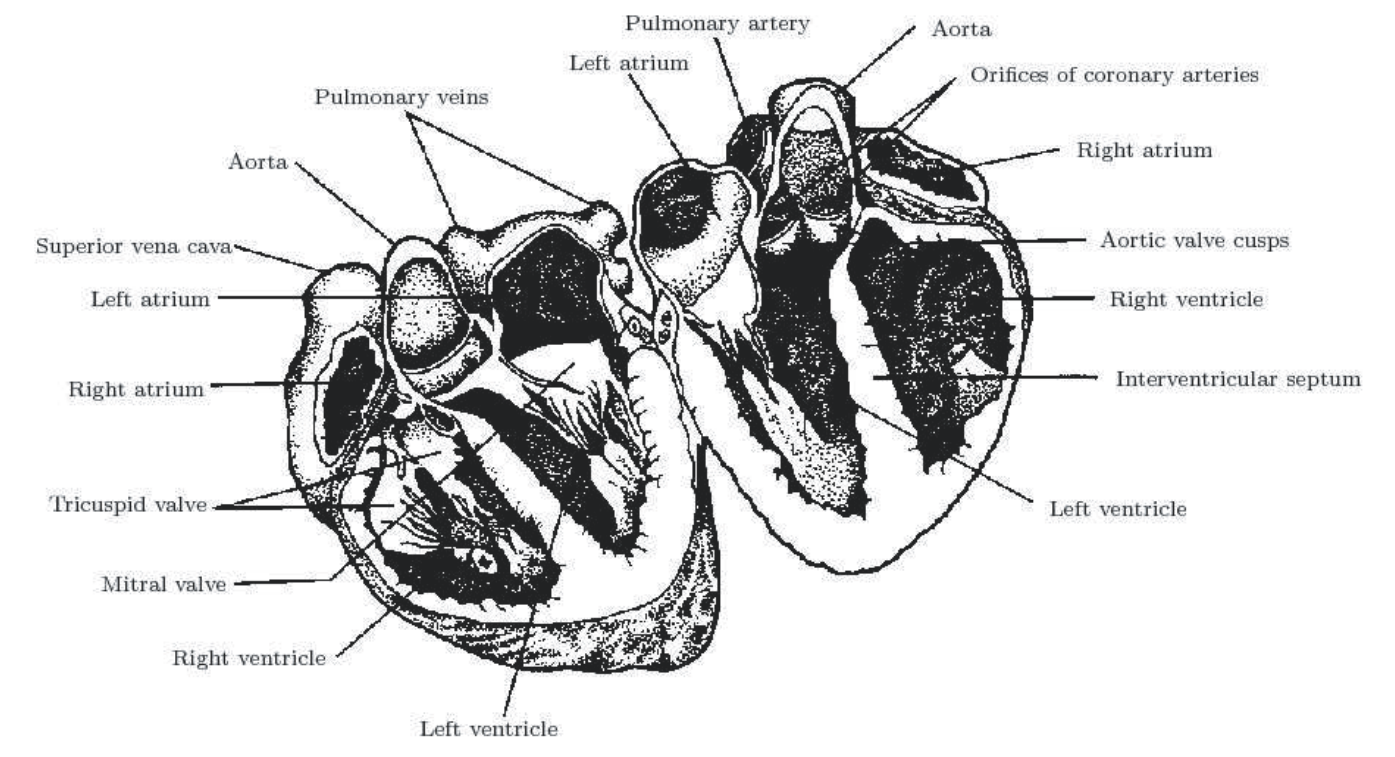
\includegraphics[width=1.0\textwidth]{media/anatomy.png}
\caption{Longitudinal cross-section of the human heart~\cite{katz_2015}}
\label{fig:anatomy}
\end{figure}

Cardiovascular disease is the leading cause of death and disability, accounting for about 40$\%$ of all human mortality~\cite{genet_2015}. Heart failure is one of the most common, costly, and deadly medical conditions, affecting more than 25 million people worldwide~\cite{mann_2015}. Better understanding the nuanced electrical and mechanical behavior of normal and pathological hearts is an important step in improving treatment for heart disease. The complexity of the mechanisms of interest, time and cost savings offered by simulation, and the high sensitivity to various patient-specific parameters make \textit{in silico} modeling an important tool in addressing heart disease.

Cardiac mechanics is one of the most mature fields in computational biomechanics. Several well-known groups have attempted to advance the field from a variety of approaches with respect to the geometry and meshing. \textit{The Living Heart Project}~\cite{baillargeon_2014, genet_2015} has arguably gained the most traction in advancing the understanding of whole-heart cardiac mechanics through simulation, albeit by using linear tetrahedra for a general 50th percentile male heart geometry (i.e., the model was not generated from medical imaging). Augustin \textit{et al.}~\cite{augustin_2016} also used linear tetrahedral finite elements, meshed from smoothed surfaces originating from MRI data. A good deal of informative research still relies on modeling simplified geometries of only the left ventricle~\cite{guccione_2005, sack_2016}, in conjunction even with cubic Hermite finite elements~\cite{mcculloch_2000}. Most modern approaches tend to generate bi-ventricular models (i.e., left and right ventricles) or whole heart models including the atria and potentially even more geometric structures.

Gurev \textit{et al.}~\cite{gurev_2015} performed mechanical simulations on a quadratic hex-dominant mixed element mesh of the human heart ventricles. The work from that group forms the basis for most of the cardiac mechanics explorations to be discussed in this chapter. The review article by Trayanova \textit{et al.}~\cite{trayanova_2011} provides an excellent summary of the components to ventricular electromechanical modeling utilized by the papers mentioned above.

The essential components to computational cardiac mechanics are described in this chapter for an implementation using conventional finite elements. Simulation results are also presented. Finally, the details of implementing the same mechanics into the polyhedral code \textit{Celeris} are discussed, along with preliminary verification results.

\section{Demonstration using Conventional Finite Elements}

The key features of a cardiac mechanics modeling implementation will be highlighted within the framework of \textit{Cardioid}~\cite{richards_2013, gurev_2015}, a highly efficient and scalable code at Lawrence Livermore National Laboratory that utilizes high performance computing for modeling the electromechanics of cardiac arrhythmia.

%%%%%%%%%%%%%%%%%%%%%%%%%%%%%%%%%%%%%%%%%%%%%%%
%%%%%%%%%%%%%%%%%%%%%%%%%%%%%%%%%%%%%%%%%%%%%%%
\subsection{Methods}
\label{Methods}

In Cardioid, quasi-static finite deformations are assumed, body forces are assumed negligible, and the stress measure of interest is the second Piola-Kirchoff stress $\bm{S}$. Thus, Equation PLACEHOLDER reduces to the following:
\begin{equation}
(F_{ik}S_{kj}),_{j} = 0
\end{equation}

In order to fully define and solve these equations, the following are specified: the mesh, material model characterization, muscle fiber orientation, solution-dependent pressure boundary conditions, and the finite element solver. Each consideration will be described in turn.

%%%%%%%%%%%%%%%%%%%%%%%%%%%%%%%%%%%%%%%%%%%%%%%
%%%%%%%%%%%%%%%%%%%%%%%%%%%%%%%%%%%%%%%%%%%%%%%
\subsubsection{Mesh Generation}
\label{Mesh Generation}

A bi-ventricular mesh is generated using the procedure described in~\chapref{2} and \chapref{3}. Namely, an MRI of an \textit{ex vivo} human heart from the CardioVascular Research~\cite{cvgg} is segmented using the software Seg3D. Since the ventricles are most responsible for the pumping action, image segmentation is restricted to those the geometric structures. A threshold segmentation is used as the initial seed to Seg3D's level set implementation. Additional tools to \textit{fill holes} or \textit{dilate-erode} are utilized before a final sweep of manual paintbrushing is employed. Following careful manual inspection, the final image mask is input to Shabaka to generate a high quality surface of the heart ventricles with a total of 50k points. Tetgen is invoked to produce a tetrahedral mesh that honors the input surface and attempts to produce high quality tetrahedra for the purposes of finite element simulations. A maximum element volume of 2 \textit{mm$^3$} was imposed. Again, quadratic tetrahedral elements are chosen over linear elements to avoid volumetric locking and/or impracticably fine meshes. The surface and mesh are shown in \figref{tetmesh} - the tetrahedral mesh has 374k elements and 595k nodes. This mesh is directly used in the Cardioid code for the purposes of finite element simulation, together with the material model and boundary conditions.

%%%%%%%%%%%%%%%%%%%%%%%%%%%%%%%%%%%%%%%%%%%%%%%
%%%%%%%%%%%%%%%%%%%%%%%%%%%%%%%%%%%%%%%%%%%%%%%
\subsubsection{Material Model}
\label{Material Model}

The cardiac tissue is assumed to exhibit an additive stress decomposition, such that $\bm{S} = \bm{S}_p + \bm{S}_a$ at any point in the model. The \textit{active stress} $\bm{S}_a$ represents the stress induced through active contraction of muscle fibers, and the \textit{passive stress} $\bm{S}_p$ the stress experienced by the underlying tissue matrix.

\textbf{Passive Stress}

The passive response of the cardiac tissue is characterized by an incompressible, transversely isotropic constitutive law by Usyk~\textit{et al.}~\cite{usyk_2002}. The strain energy density functional is given by:
\begin{gather}
W = \frac{C}{2}\left(e^Q -1\right) \\
Q = b_{ff} E^2_{ff} + b_{ss} E^2_{ss} + b_{nn} E^2_{nn} + b_{fs}\left(E^2_{fs} + E^2_{sf}\right) + b_{fn}\left(E^2_{fn} + E^2_{nf}\right) + b_{ns}\left(E^2_{ns} + E^2_{sn}\right)
\end{gather}
where $\bm{E}$ is the Green-Lagrange strain tensor expressed in a local orthonormal coordinate system with axes parallel to the local fiber, sheet, and sheet-normal $(f,s,n)$ directions, and where $C$, $b_{ff}$, $b_{ss}$, $b_{nn}$, $b_{fs}$, $b_{fn}$, and $b_{ns}$ are material parameters.

Incompressibility is fully enforced by solving for pressure unknowns as Lagrange multipliers in addition to nodal unknowns. The deviatoric and volumetric portions of the strain energy are separated within a framework enforcing full incompressibility. Rather than defining the passive stress as simply $\bm{S}_p = \frac{\partial W}{\partial \bm{E}}$, the passive stress becomes:
\begin{equation}
\bm{S}_p= 2\frac{\partial{\tilde{W}(\tilde{\bm{C}})}}{\partial{\bm{C}}} - pJ\bm{C}^{-1}
\end{equation}
where $\tilde{W}(\tilde{\bm{C}})$ is the deviatoric component of the strain energy functional, $J = \text{det}(\bm{F})$, and $\tilde{\bm{C}} = J^{-2/3}\bm{C}$. More details regarding the enforcement of incompressibility can be found in Gurev \textit{et al.}~\cite{gurev_2015}.

\textbf{Active Stress}

The active stress is defined as :
\begin{equation}
\bm{S}_a = \sigma_a \bm{f} \bm{f}^{T}
\label{eqn:active}
\end{equation}
where $\bm{f}$ is the muscle fiber direction and ${\sigma_a}$ is the scalar active tension induced in the fiber direction. The vector $\bm{f}$ here may refer to the fiber orientation either in the reference configuration or the current configuration - within the Cardioid framework it will refer to the direction in the reference configuration.

The active tension model by Lumens \textit{et al.}~\cite{lumens_2009} is used to determine the active tension $\sigma_a$, in the following manner:
\begin{align}
\frac{d\bm{w}}{dt} = \bm{q}(\bm{w}; t_a, \lambda) \\
\sigma_a \equiv \sigma_a(\bm{w}; t_a, \lambda)
\end{align}
The scalar active tension depends on state variables $\bm{w}$ involving the sarcomere length of the muscle cells, the time of electrical activation of those cells $t_a$, and the muscle fiber stretch $\lambda$ in the direction of $\bm{f}$. Namely, $\lambda = (\bm{f}\bm{C}\bm{f}^T)^{1/2}$. The state variables are updated explicitly within the constitutive update subroutine. Further details on the state variables $\bm{w}$ and the way in which they are updated via $\bm{q}$ can be found in the work by Lumens~\textit{et al.}~\cite{lumens_2009}.

The activation time $t_a$ at each integration point is gathered from the results of the electrophysiology portion of the Cardioid code~\cite{richards_2013}. Specifically, an electrostatics problem is solved numerically for time-varying voltages, and the the activation time is determined based on when the voltage at each location passes a certain threshold. In this manner, a one-way coupling is imposed, in which the mechanics code depends on the electrophysiology results, but not vice versa. A fixed beat duration $t_b$ is assumed, such that the myofilament model excites and contracts for the $n$th beat at time $nt_b + t_a$. Activation times are read in to the mechanics code for each of the integration points of the mesh as a field variable (see \figref{supp1}).

\begin{figure}[ht]
\centering
\subfigure[]{%
		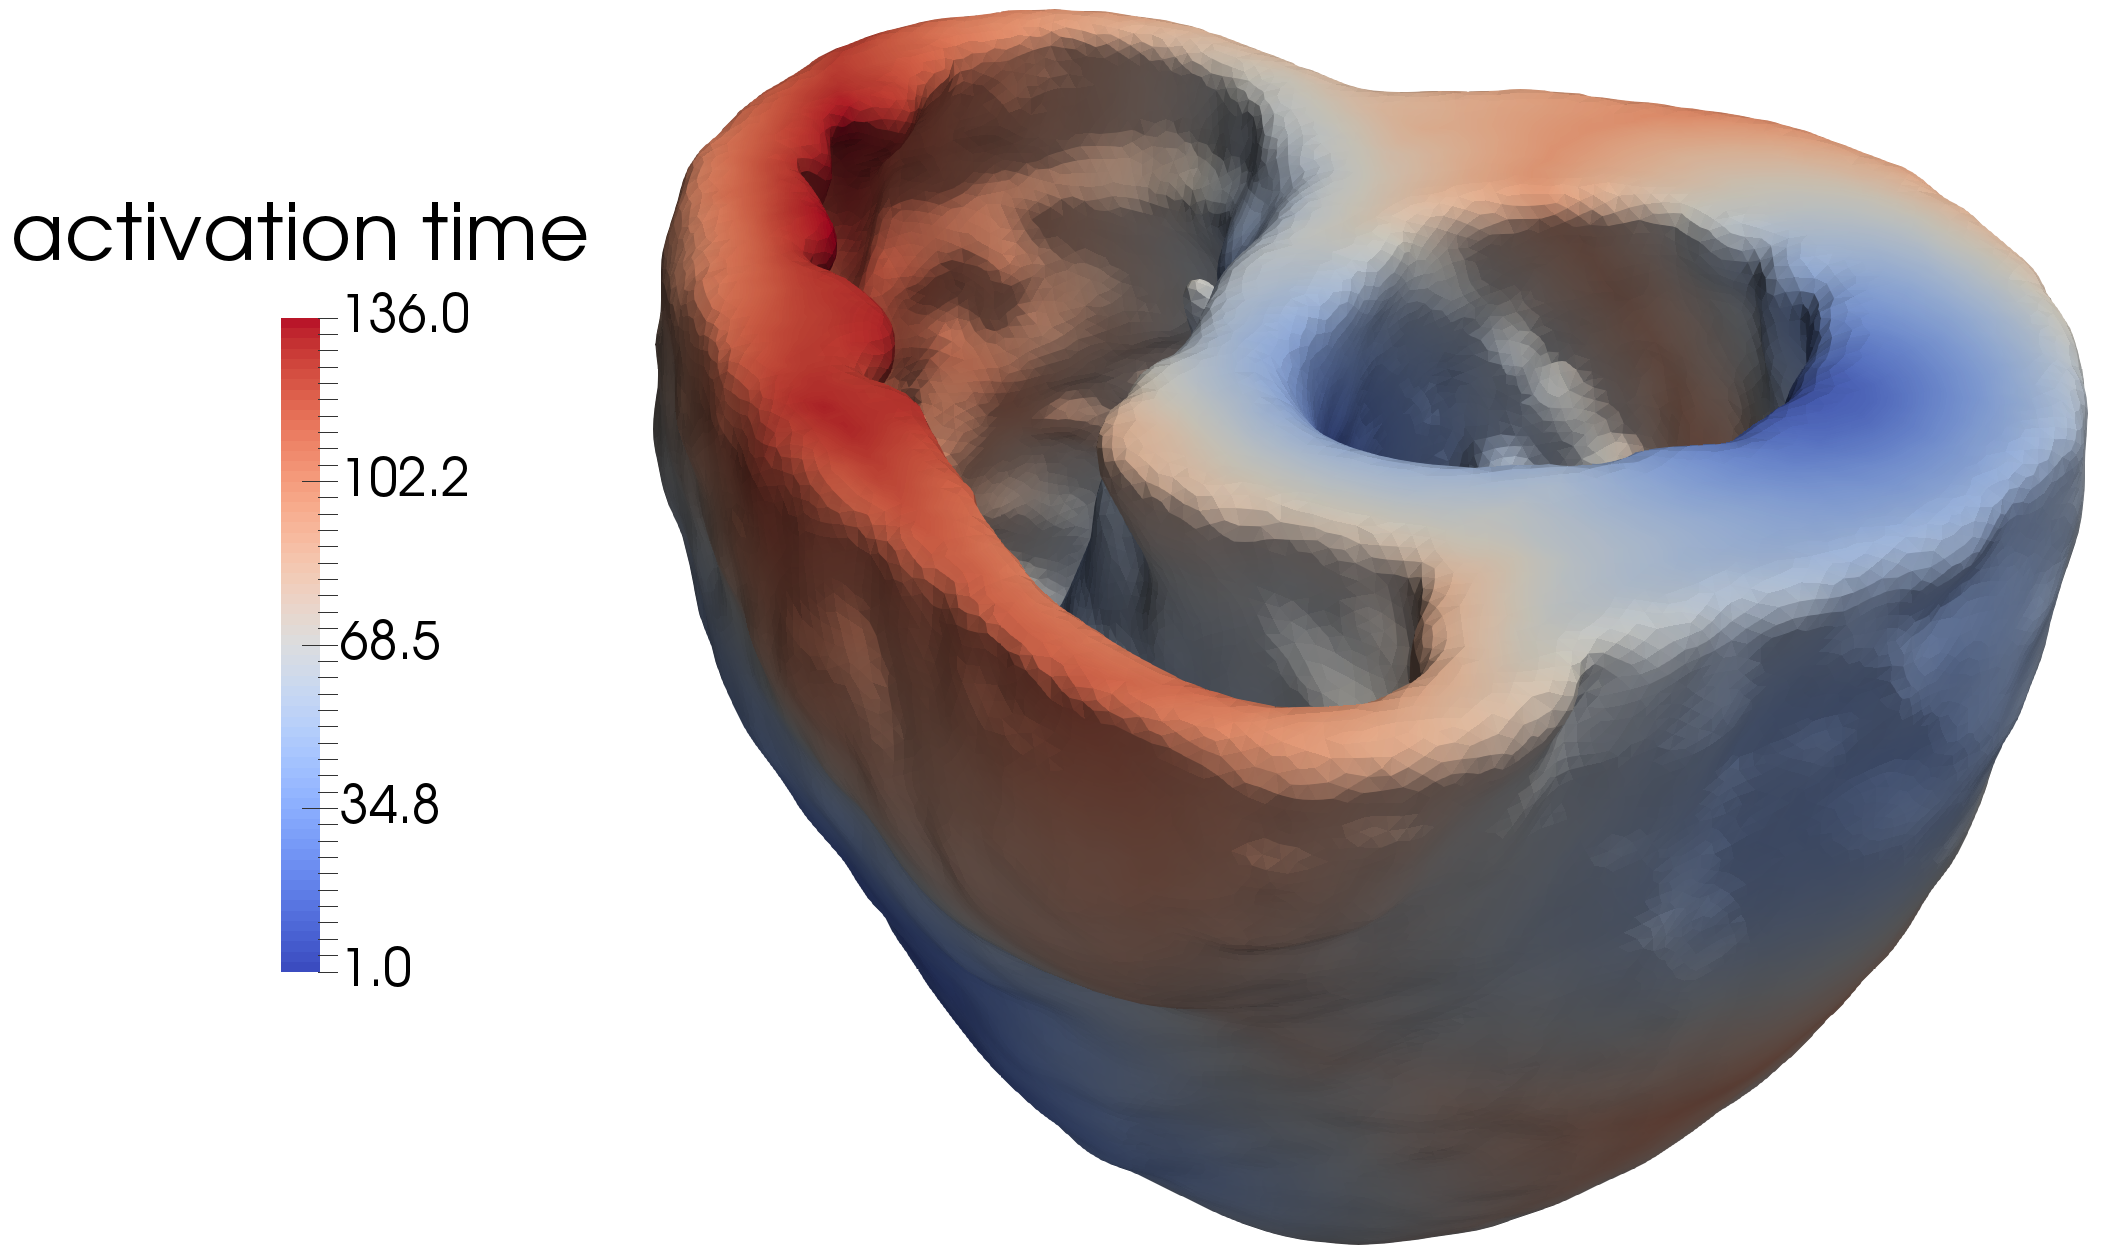
\includegraphics[scale=0.081]{media/4-cardioid/2-activationtime.png}
\label{fig:supp1}}
\subfigure[]{%
		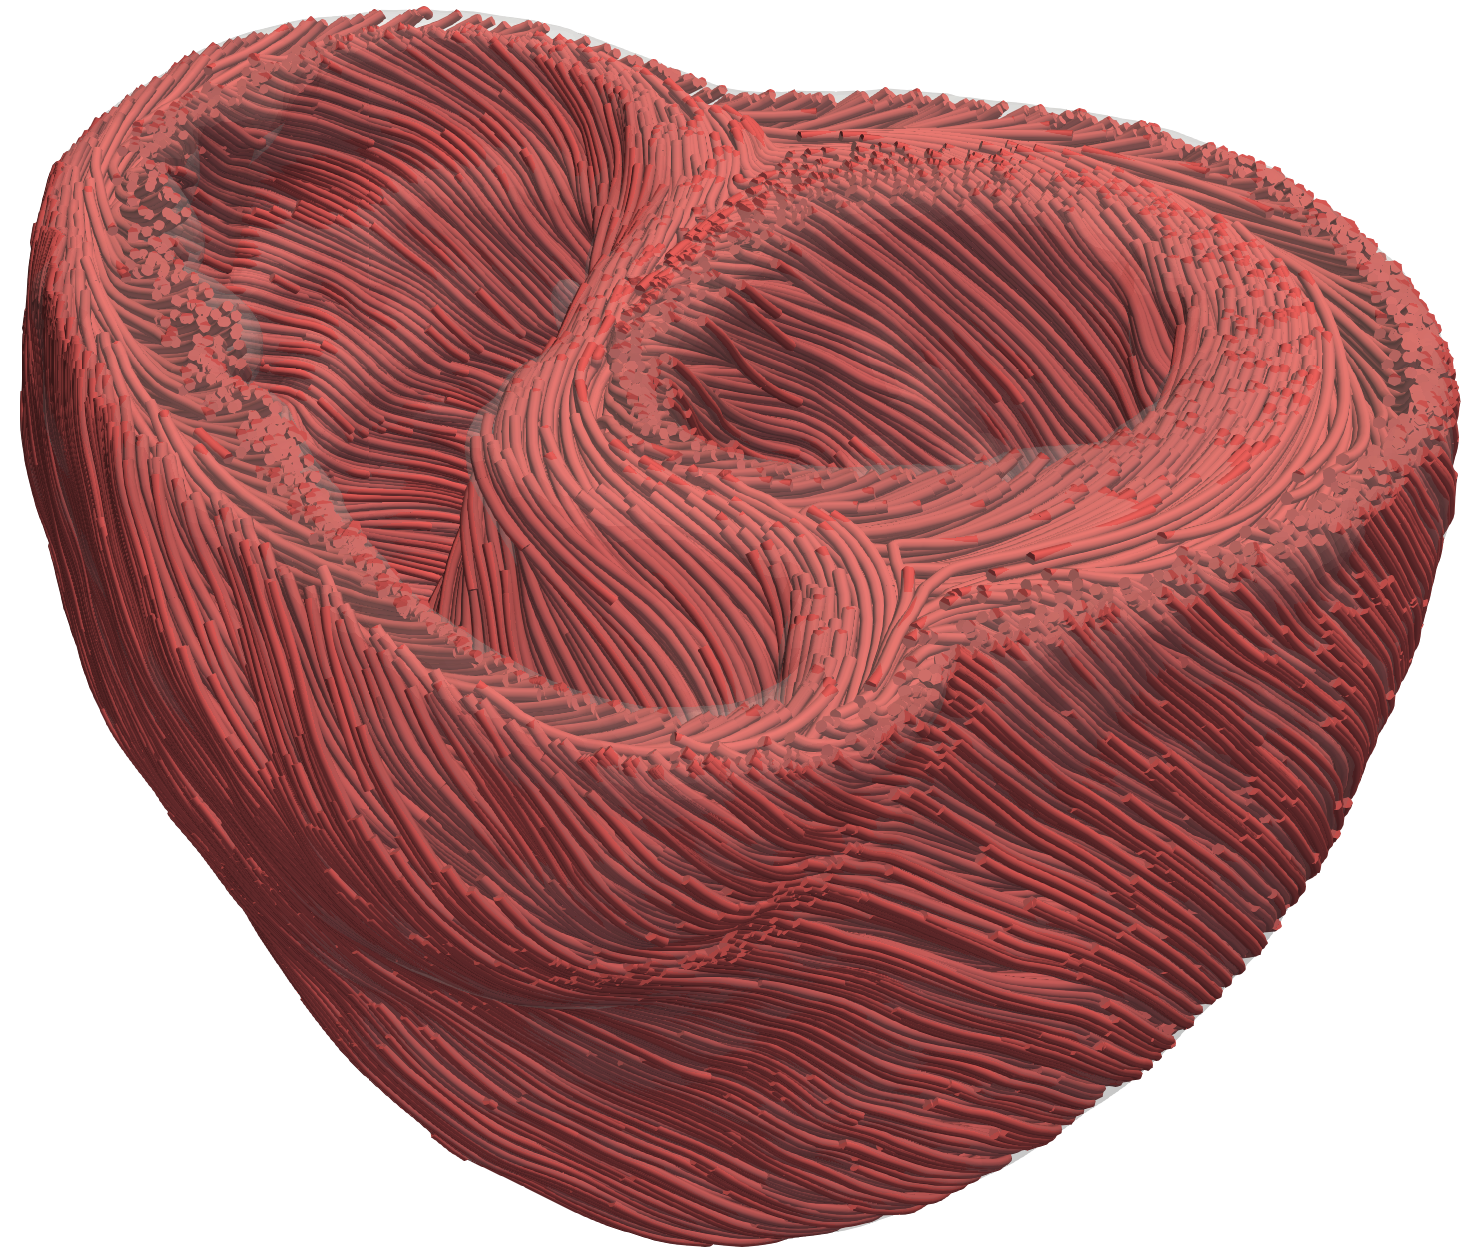
\includegraphics[scale=0.081]{media/4-cardioid/3-fibers.png}
\label{fig:supp2}}
\subfigure[]{%
		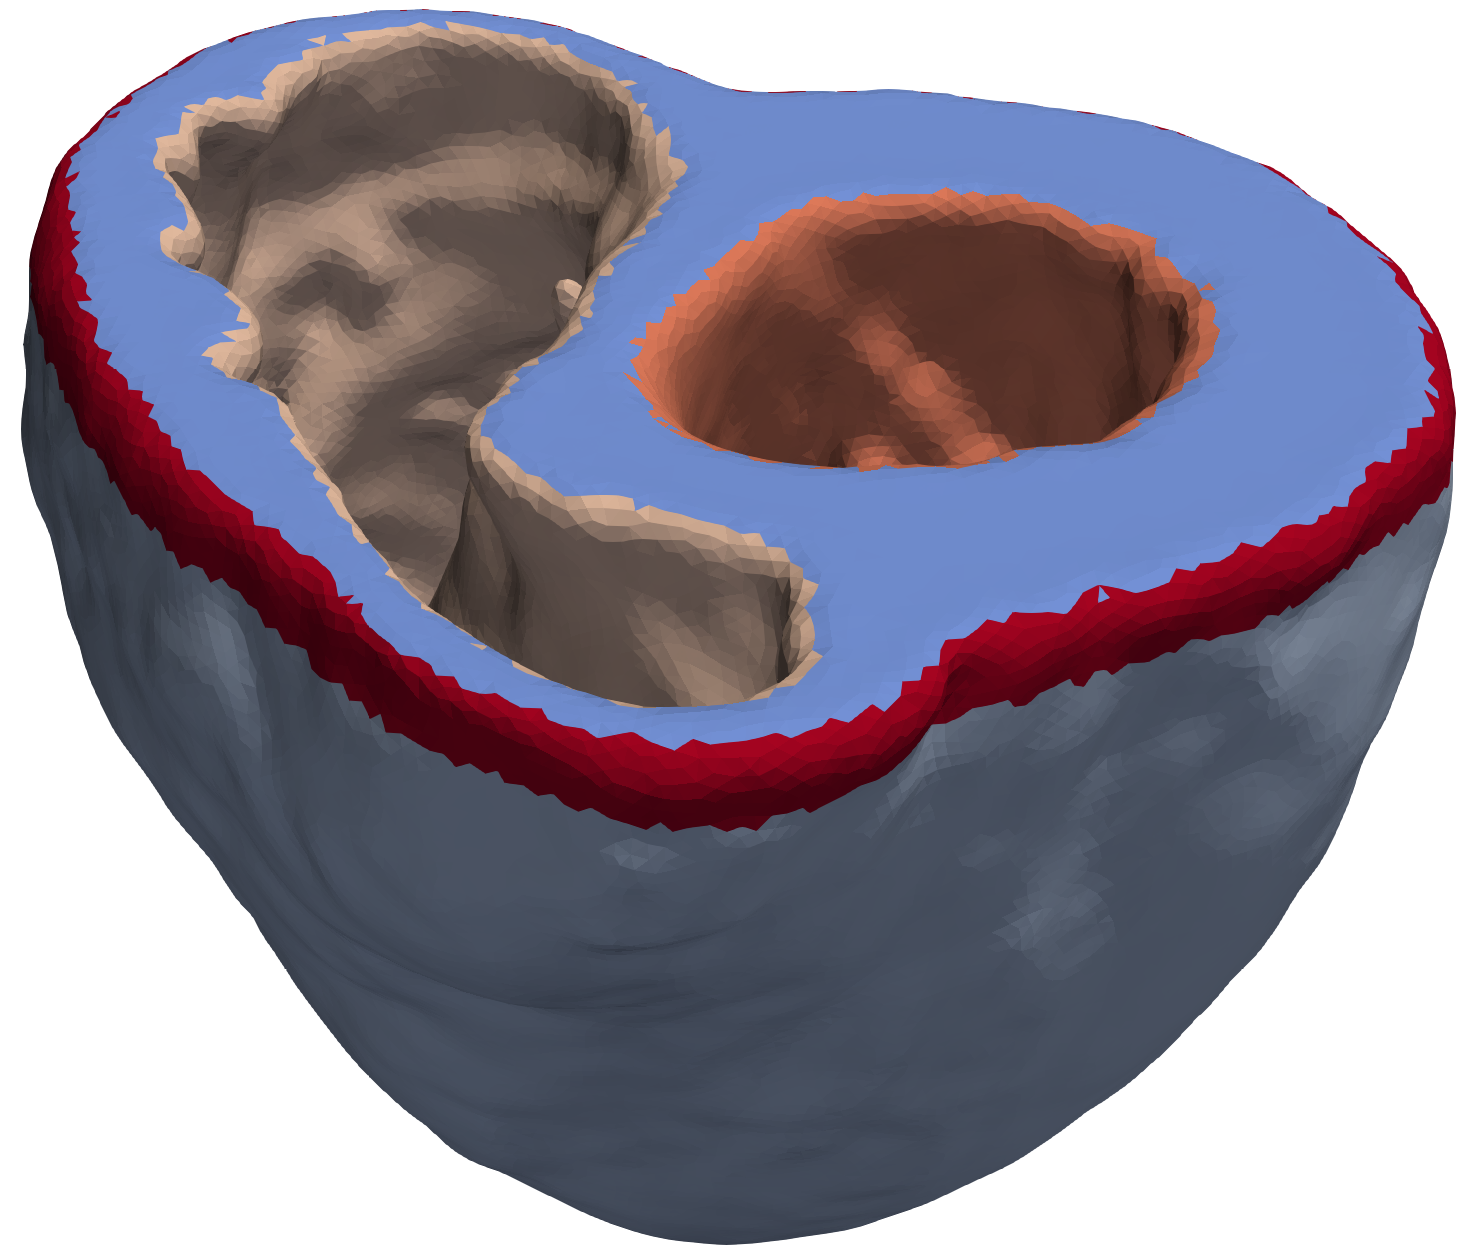
\includegraphics[scale=0.081]{media/4-cardioid/4-tagged.png}
\label{fig:supp3}}
%
\caption{Mechanics modeling considerations: (a) muscle fiber orientations, (b) electrical activation times, and c) surface tagging and prescription of corresponding boundary conditions.}
\label{fig:supp}
\end{figure}

Both the passive and active portions of the constitutive model depend on muscle fiber orientation. Fiber orientations may be generated directly from DTMRI data, but require the difficult tasks of tensor denoising, smoothing, and interpolation in the presence of noisy data. Additionally, DTMRI data is more timely, more expensive, and may not always be available. The Cardioid implementation opts for the more popular \textit{rule-based approach}, in which fiber orientations are artificially generated based on the input mesh, to mimic the orientations exhibited in reality. The implementation utilizes the algorithm by Bayer \textit{et al.}~\cite{bayer_2012}, involving solving several elliptic boundary value problems in succession. Specifically, Laplace's equation $\nabla^2\phi = 0$ is solved four times, each with different Dirichlet boundary conditions (see~\figref{bayer}).

\begin{figure}[ht]
\centering
		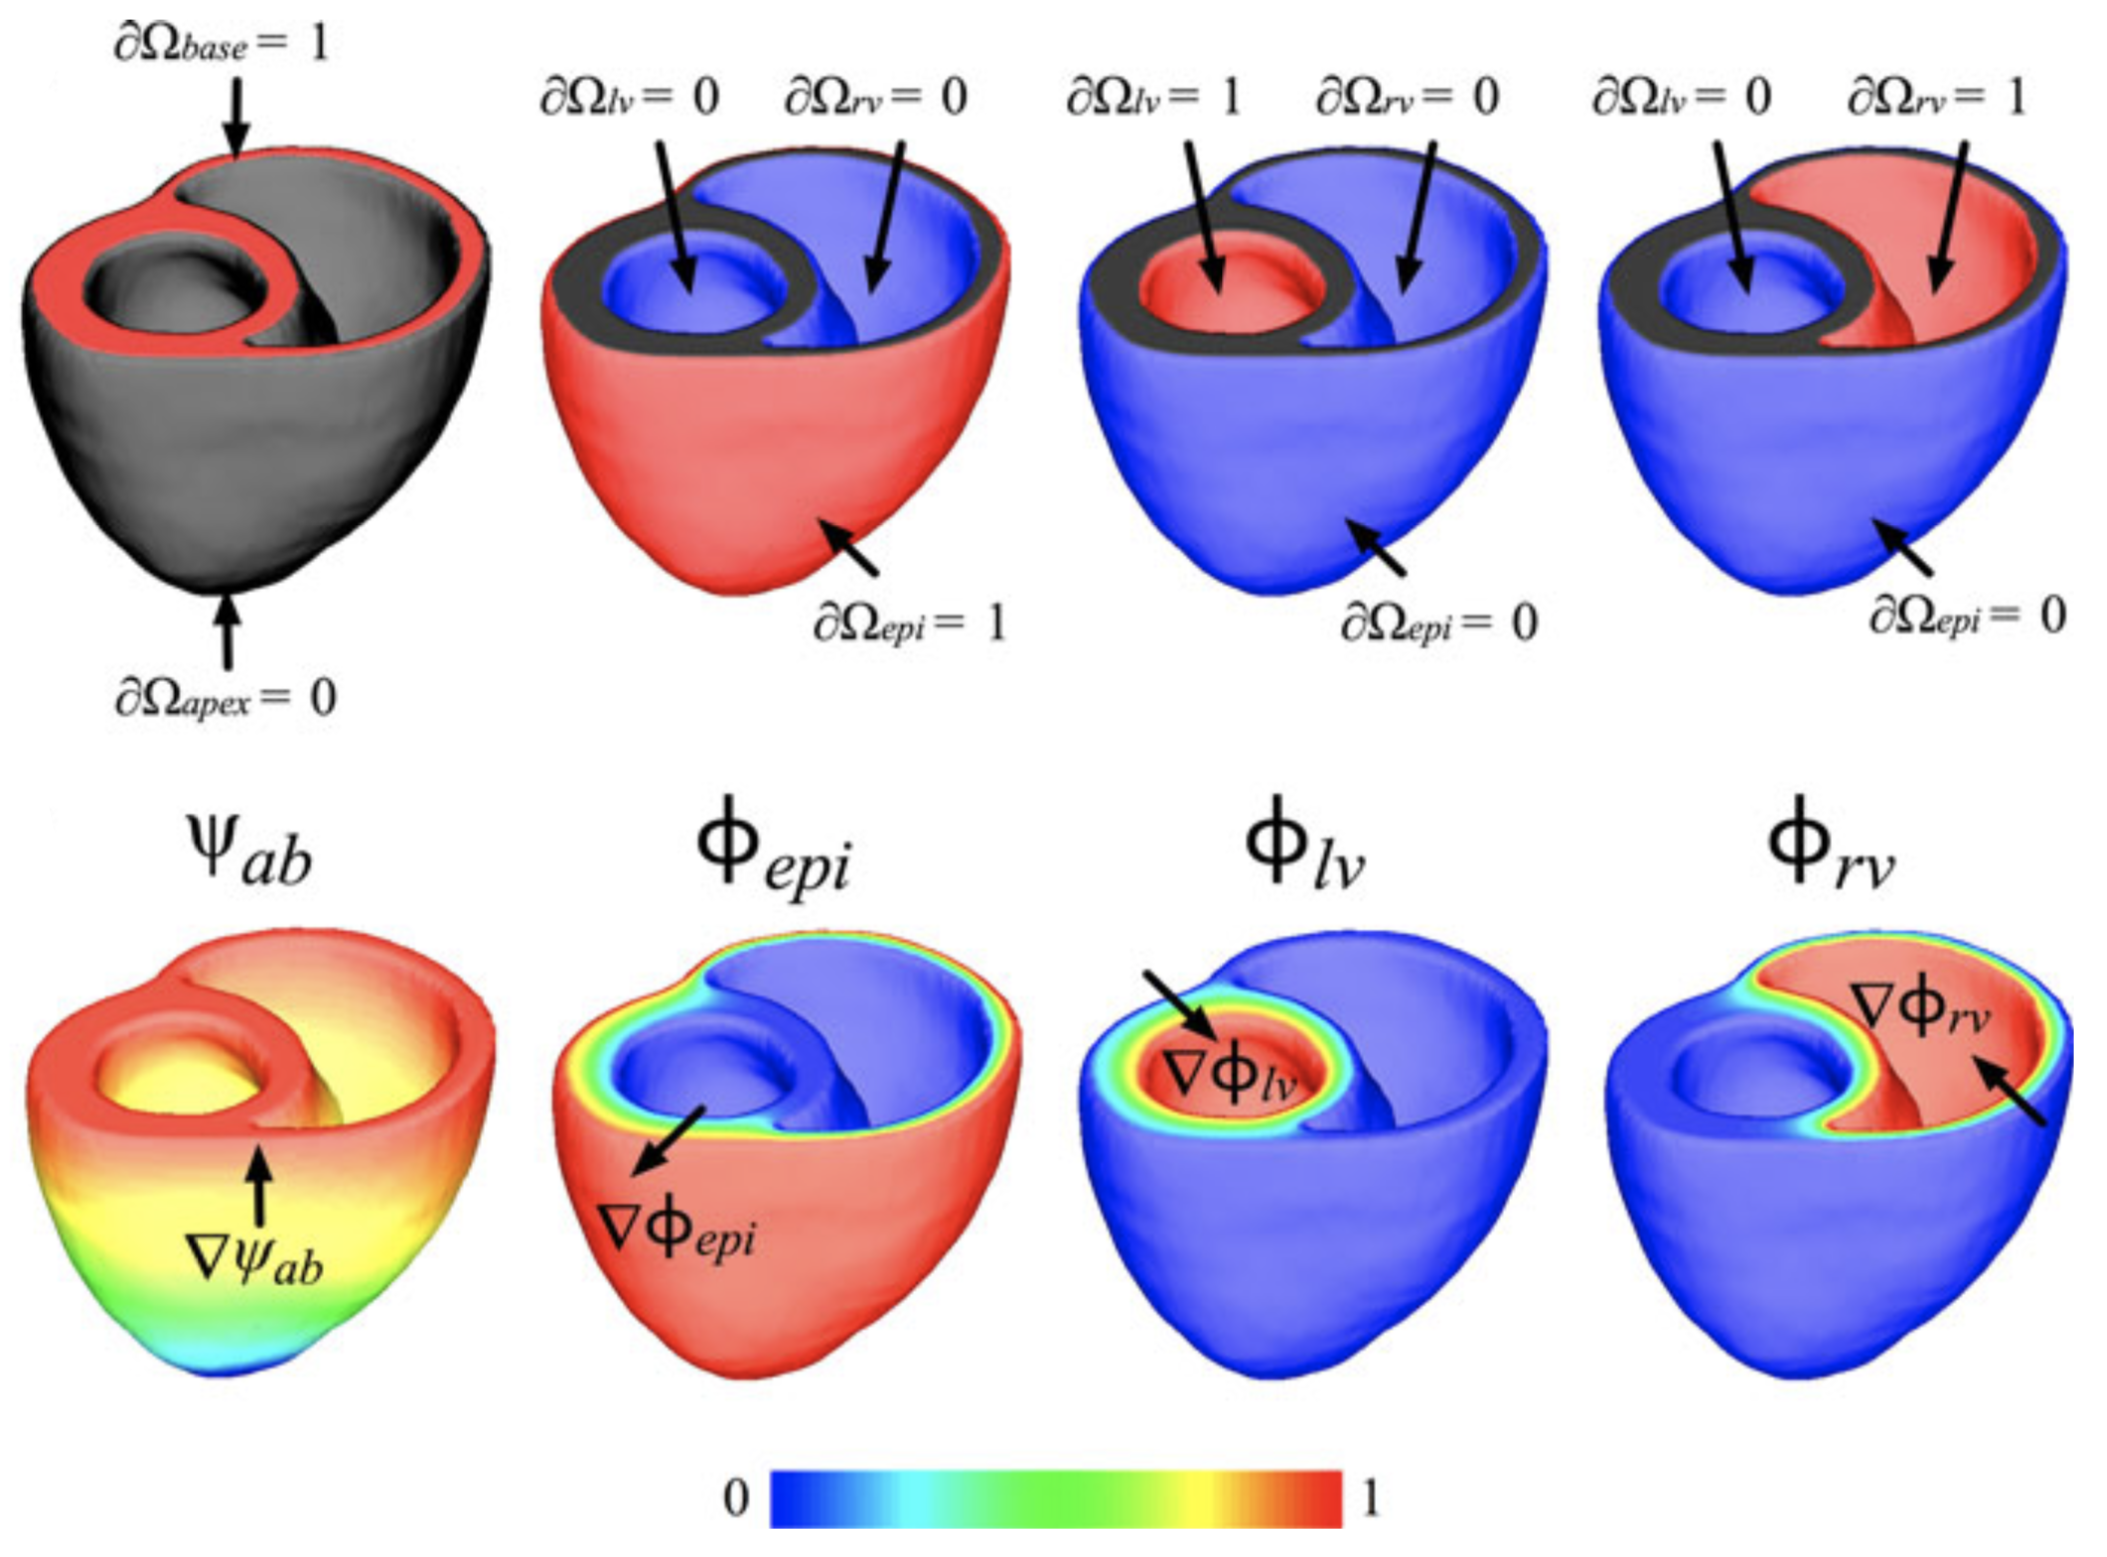
\includegraphics[scale=0.3]{media/bayer.png}
\caption{Boundary conditions and resulting scalar solutions to Laplace's equation. The gradients of the solutions are used to construct the rule-based fiber orientations~\cite{bayer_2012}}
\label{fig:bayer}
\end{figure}

The gradients of these solutions inform the construction of orthotropic fiber orientations at each solution point. Finally, fiber orientations are interpolated at the junctions between the LV, RV, and septum to ensure that the fiber direction changes smoothly and continuously throughout the entire myocardium. The details by which the gradients are used to construct the fiber orientations and by which orientations are interpolated are explained in the work of Bayer~\textit{et al.}~\cite{bayer_2012}. The Laplace solves are performed using the highly parallelized finite element code \textit{MFEM}~\cite{mfem-library} on the same input quadratic tetrahedral mesh to be used for the mechanics simulation. The algorithm is robust for various geometries and compares well with fiber orientations generated directly from DTMRI data. The computed fiber orientations for the mesh of interest are shown in \figref{supp2}.

%%%%%%%%%%%%%%%%%%%%%%%%%%%%%%%%%%%%%%%%%%%%%%%
%%%%%%%%%%%%%%%%%%%%%%%%%%%%%%%%%%%%%%%%%%%%%%%
\subsubsection{Boundary Conditions}
\label{Boundary Conditions}

Fluid flow and fluid-structure interaction are not yet implemented in the Cardioid code, so a volume constraint is imposed to mimic the effect of blood flow in the ventricles. The volumes of the ventricle cavities are calculated based on a lumped circulatory model by Kerckhoffs \textit{et al.}~\cite{kerckhoffs_2006}, which are in turn used to determine the time-varying, solution-dependent pressure boundary conditions.

A system of coupled ODEs describing the time evolution of the left ventricle volume $V_{LV}$ and the right ventricle volume $V_{RV}$ for the circulatory model can be written in the form:
\begin{align}
\frac{d\bm{w}_{c}}{dt} = \bm{q}_c(\bm{w}_c, p_{LV}, p_{RV}; t) \\
\frac{dV_{LV}}{dt} = g_{LV}(p_{LV}, \bm{w}_c; t) \\
\frac{dV_{RV}}{dt} = g_{RV}(p_{RV}, \bm{w}_c; t)
\end{align}
where $\bm{w}_c$ is the vector of state variables for the circulatory model, $p_{LV}$ and $p_{RV}$ are the  pressures inside the left and right ventricles, and $\frac{dV_{LV}}{dt}$ and $\frac{dV_{RV}}{dt}$ represent the change in blood volume into the each of the ventricles. The right hand side functions $\bm{q}_c$, $g_{LV}$, and $g_{RV}$ are described in detail in Kerckhoffs~\textit{et al.}~\cite{kerckhoffs_2006}. This paradigm assumes both that the blood is incompressible, and that the pressure is uniform within each ventricle. For each time step, the ventricular volumes are calculated from the circulatory model and imposed as constraints on the finite element mesh to determine the corresponding ventricular pressures. The details by which the pressures are computed from the volume constraint are detailed in Gurev~\textit{et al.}~\cite{gurev_2015}. The circulatory model is shown in~\figref{bcs}.
\begin{figure}[ht]
\centering
		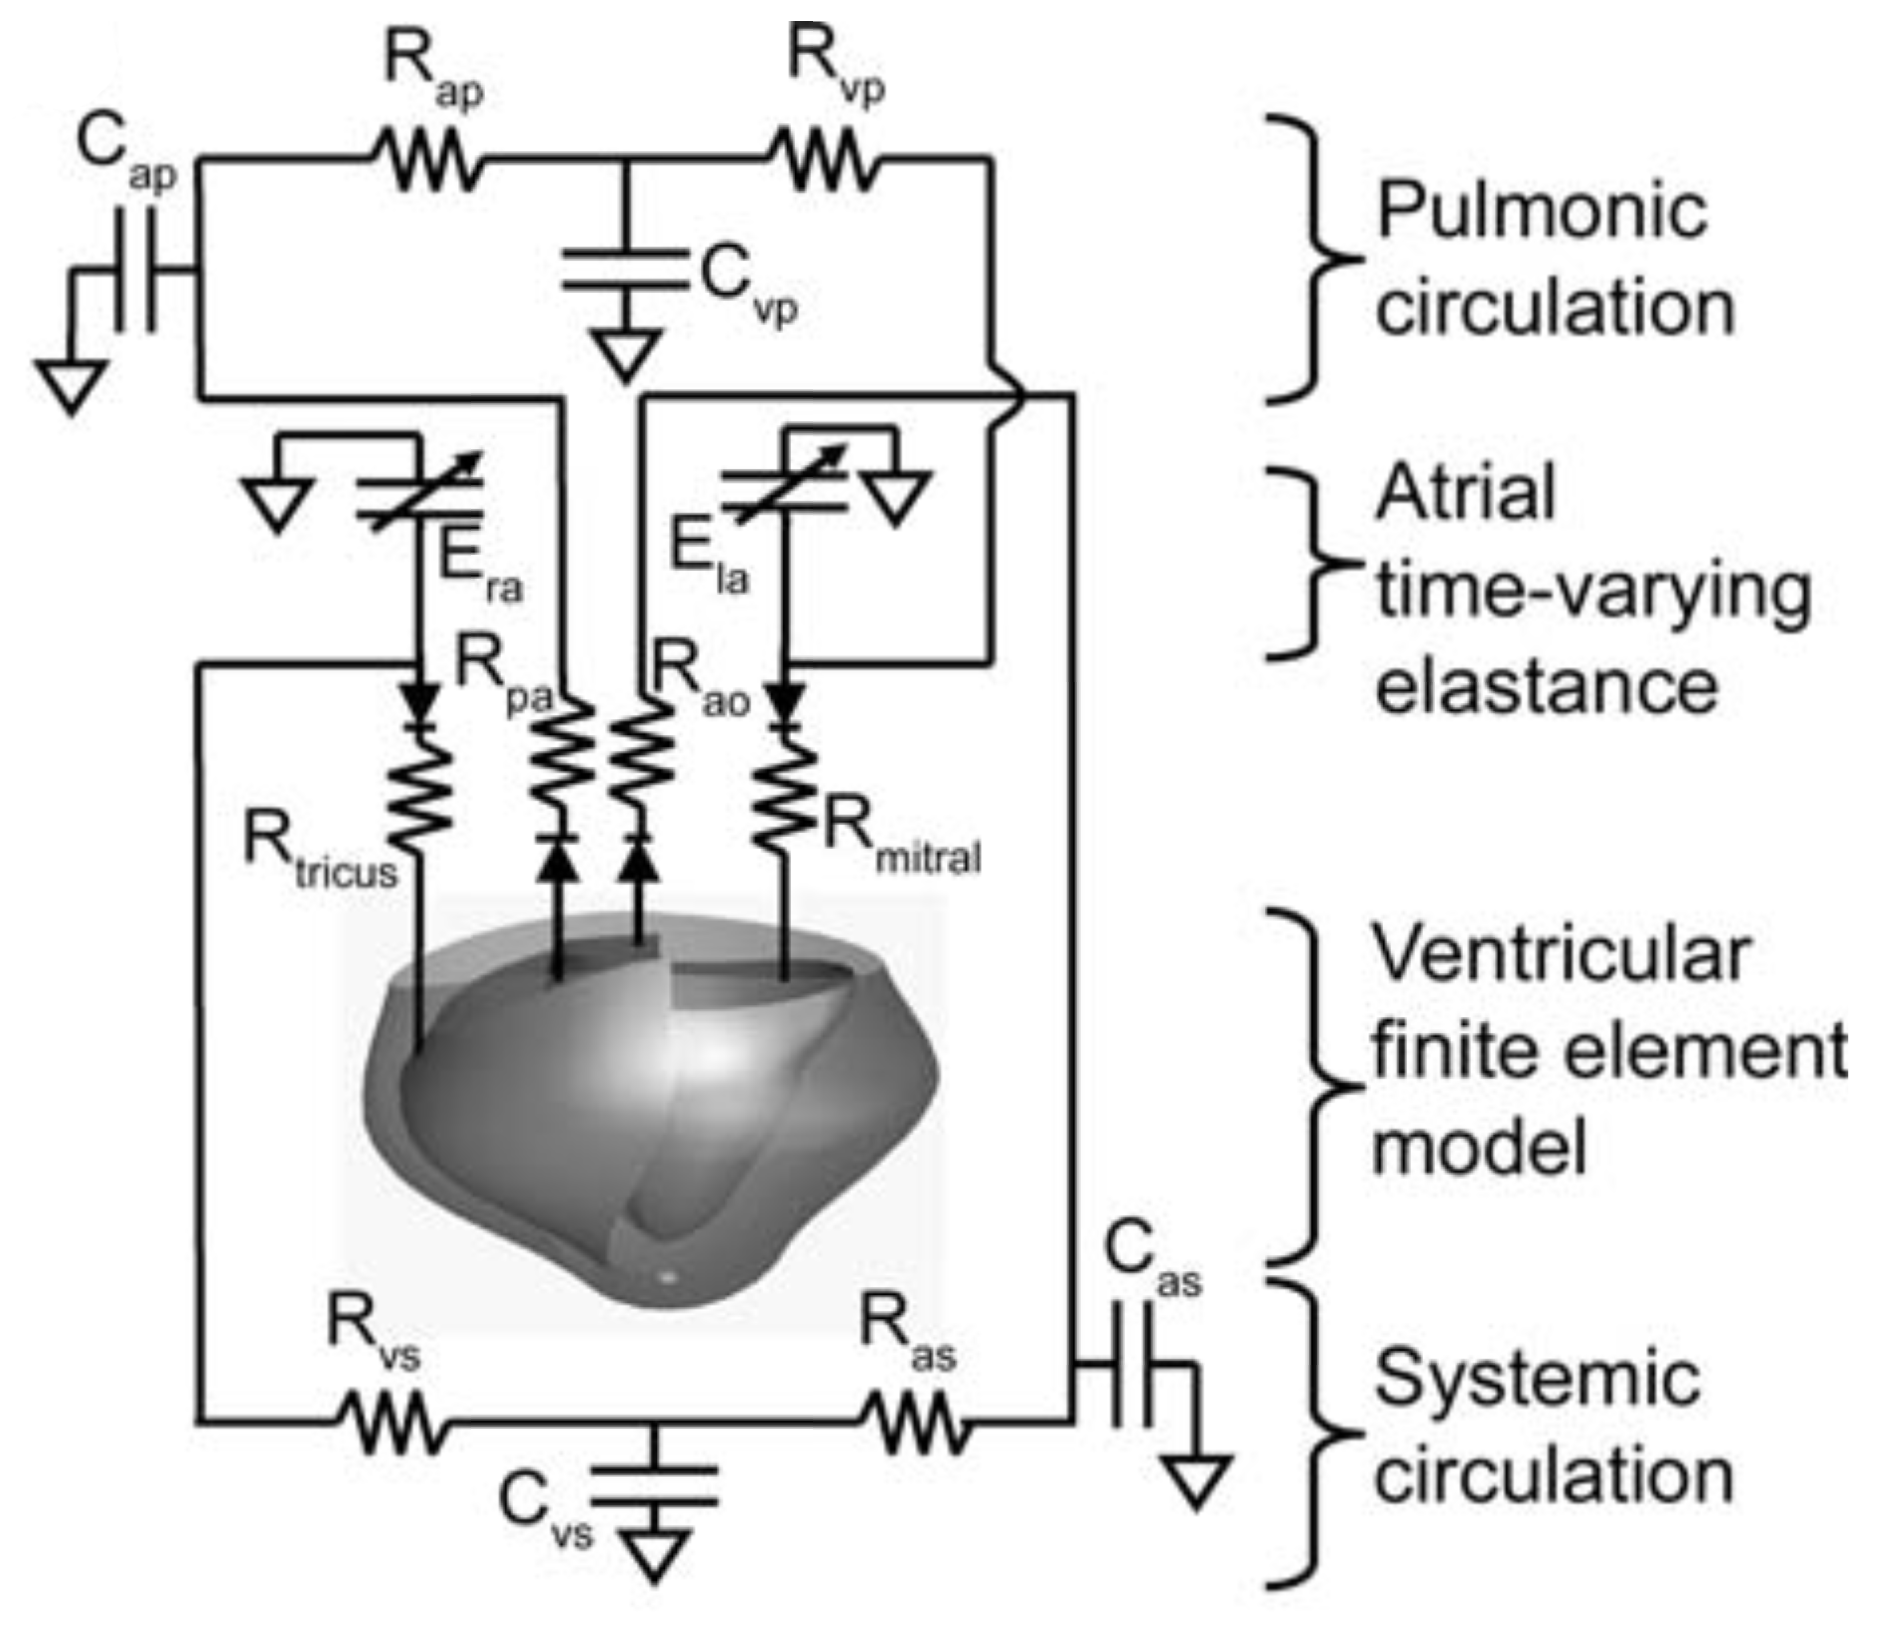
\includegraphics[scale=0.3]{media/bcs.png}
\caption{Lumped circulatory model of Kerckhoffs\textit{et al.}~\cite{kerckhoffs_2006}. Variables shown in the schematic are parameters in the coupled system of ODEs that are solved for ventricular volumes.}
\label{fig:bcs}
\end{figure}

In order to avoid highly nonlinear solutions at the beginning of the simulation, initial pressures are applied linearly in the first 100 ms prior to ``turning on'' the active contraction. One may think of the first 100 ms as a period in which a residual stress is applied prior to imposing the loading and boundary conditions of interest for the remainder of the simulation.

Displacement boundary conditions are enforced such that the base of the heart is not allowed to move out of plane, and that a strip of the epicardium near the base experiences zero displacements in all directions. In order to enforce these displacement and pressure BCs, the appropriate surfaces must be identified. Identification of the base, epicardium, left ventricle, and right ventricle is actually a necessary intermediate step in generating fiber directions, so those boundary condition tags are already available (see~\figref{supp3}).

%%%%%%%%%%%%%%%%%%%%%%%%%%%%%%%%%%%%%%%%%%%%%%%
%%%%%%%%%%%%%%%%%%%%%%%%%%%%%%%%%%%%%%%%%%%%%%%
\subsubsection{Solver}
\label{Solver}

The quadratic tetrahedral mesh described previously is used together with the material model and boundary conditions to perform conventional finite element simulations using the freely available \textit{oomph-lib}~\cite{oomph}. 

In the interest of solving problems with fine discretizations, Gurev \textit{et al.} avoid direct solvers of the linear system in Cardioid due to their poor scalability. Instead they employ a Krylov subspace iterative solver, which is more suitable for large scalable problems. The existence of active contraction creates saddle-points in the linear system that are addressed with a novel preconditioner. The details of the linear solver may be found in the publication by Gurev \textit{et al.}.

The simulation was performed on the \textit{Surface} computing platform at Lawrence Livermore National Laboratory. The Moab schedule manager was used to submit the job to be run on 50 nodes, with 16 cores per node, for a total of 800 processes. With an assumed beat duration of 1000 $ms$ for a healthy human heart (i.e., 60 beats per minute), the simulation is run from time 0 to 5100 ms with a time increment $\Delta t = 1 ms$. The simulation completed roughly one heartbeat per 24 hours of wall clock time. As mentioned previously, the first 100 ms are used to linearly apply the initial pressures for the simulation. The first beat is discarded as the heart reaches a dynamic steady state, and thus four full beats of a healthy human heart are extracted from the results.

%%%%%%%%%%%%%%%%%%%%%%%%%%%%%%%%%%%%%%%%%%%%%%%
%%%%%%%%%%%%%%%%%%%%%%%%%%%%%%%%%%%%%%%%%%%%%%%
\subsection{Results}
\label{Results}

Simulation results for the problem described in this chapter are shown in~\figref{pv} and~\figref{snaps}. \figref{pv1} is known as a \textit{P-V loop} of the left ventricle, and \figref{pv2} is a time history plot of the pressure in the left and right ventricles. \figref{pv1} demonstrates the four stages of the cardiac cycle: 1) isovolumetric contraction from label a to b, ventricular ejection of blood from label b to c, isovolumetric relaxation from label c to d, and ventricular filling from label d to a. Isovolumetric contraction and ventricular ejection comprise what is known as \textit{systole}, in which the ventricles are contracting, whereas isovolumetric relaxation and ventricular filling are known as \textit{diastole}, in which the ventricles are relaxing. The labels in \figref{pv1} correspond to the panels in~\figref{snaps} showing the deformed mesh with an overlay of fiber stretch $\lambda$. During a cycle, fiber stretch ranges from 0.6 to 1.4, certainly justifying the finite deformation simulatoin approach. The results closely match those in Gurev~\textit{et al.}~\cite{gurev_2015}, in which a different heart geometry and electrophysiology is used, indicating a robustness to the workflow. The full video of four heartbeats played at one quarter speed may be found at \href{youtu.be/RtQKEjdR4MU}. A robust workflow has thus been demonstrated for performing bi-ventricular cardiac mechanics simulations. Additional validation of the results, quantitiative metrics for the quality of the solution, and sensitivity studies of the simulation parameters would be the next steps and would certainly be informative.

\begin{figure}[ht]
\centering
\subfigure[]{%
		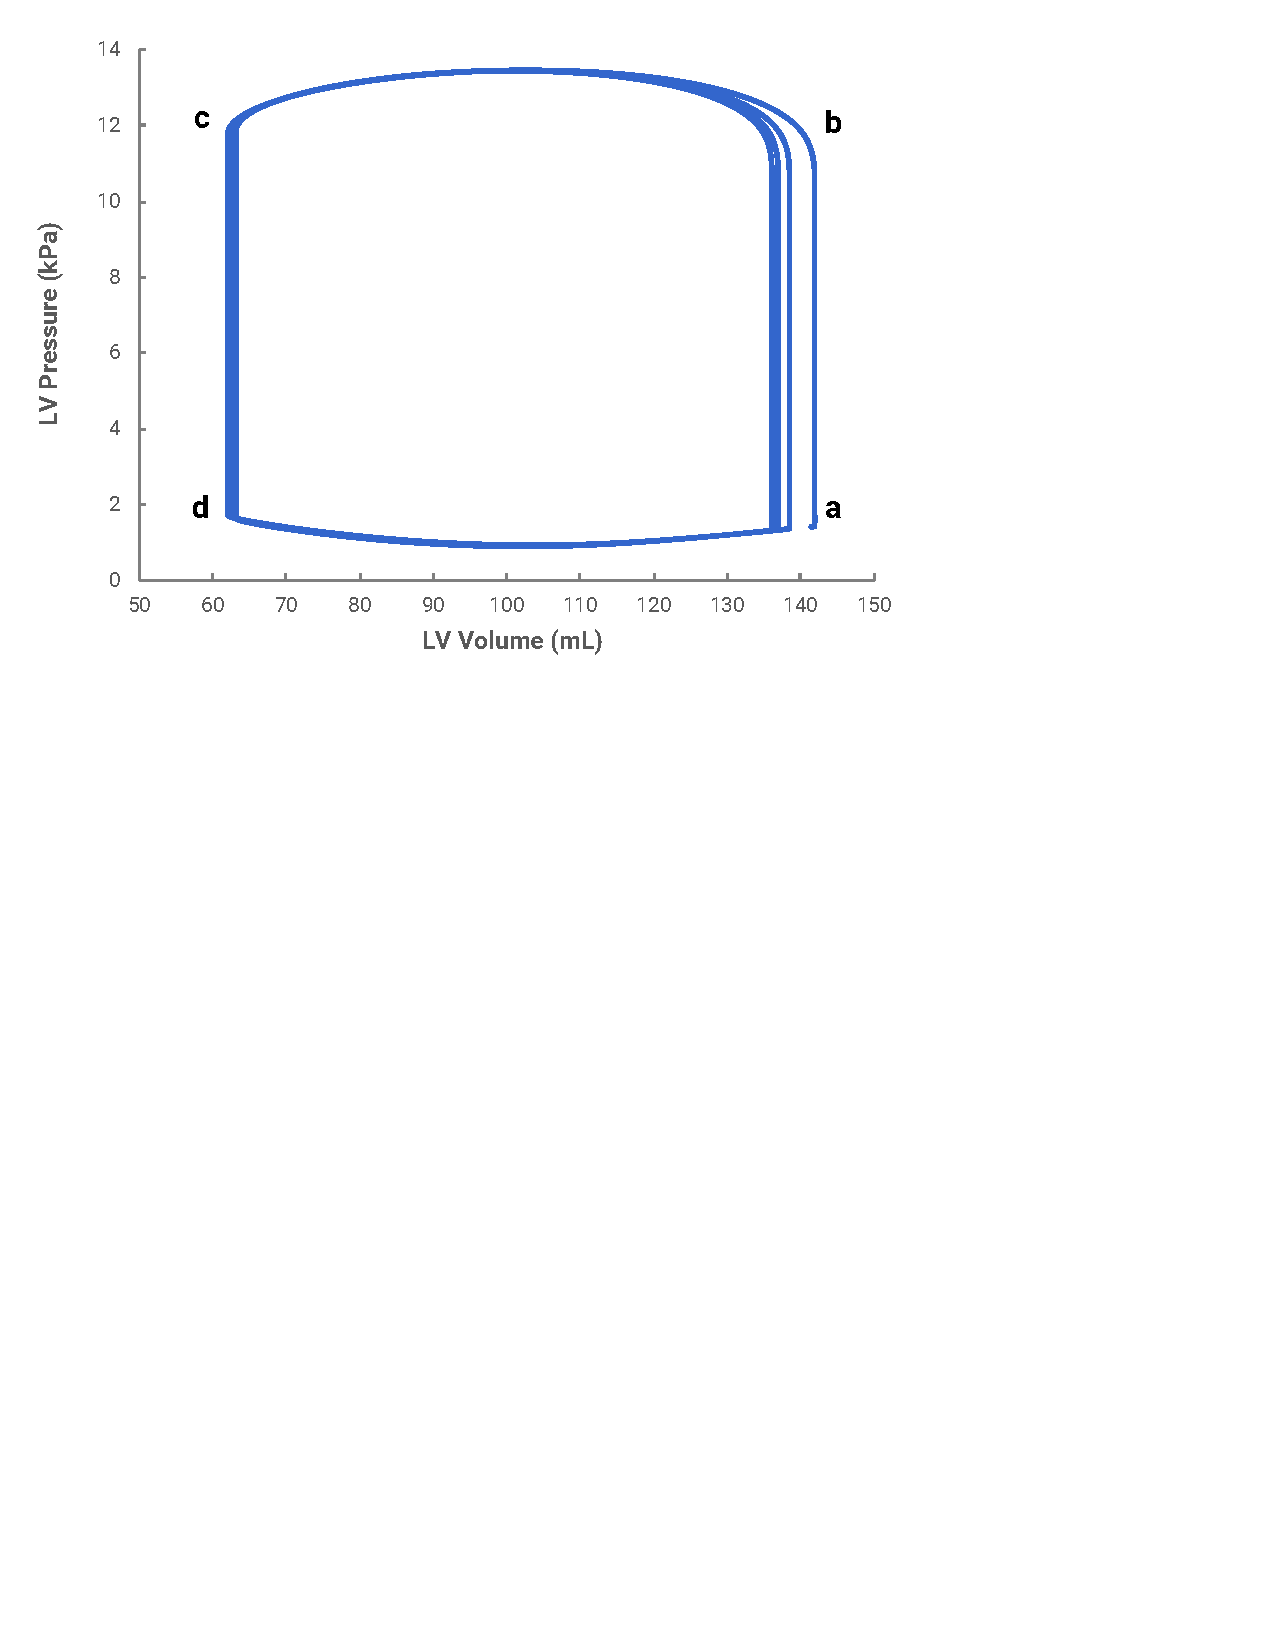
\includegraphics[scale=0.5]{media/4-cardioid/5-pv/pressure_volume-1.pdf}
\label{fig:pv1}}		
\subfigure[]{%
		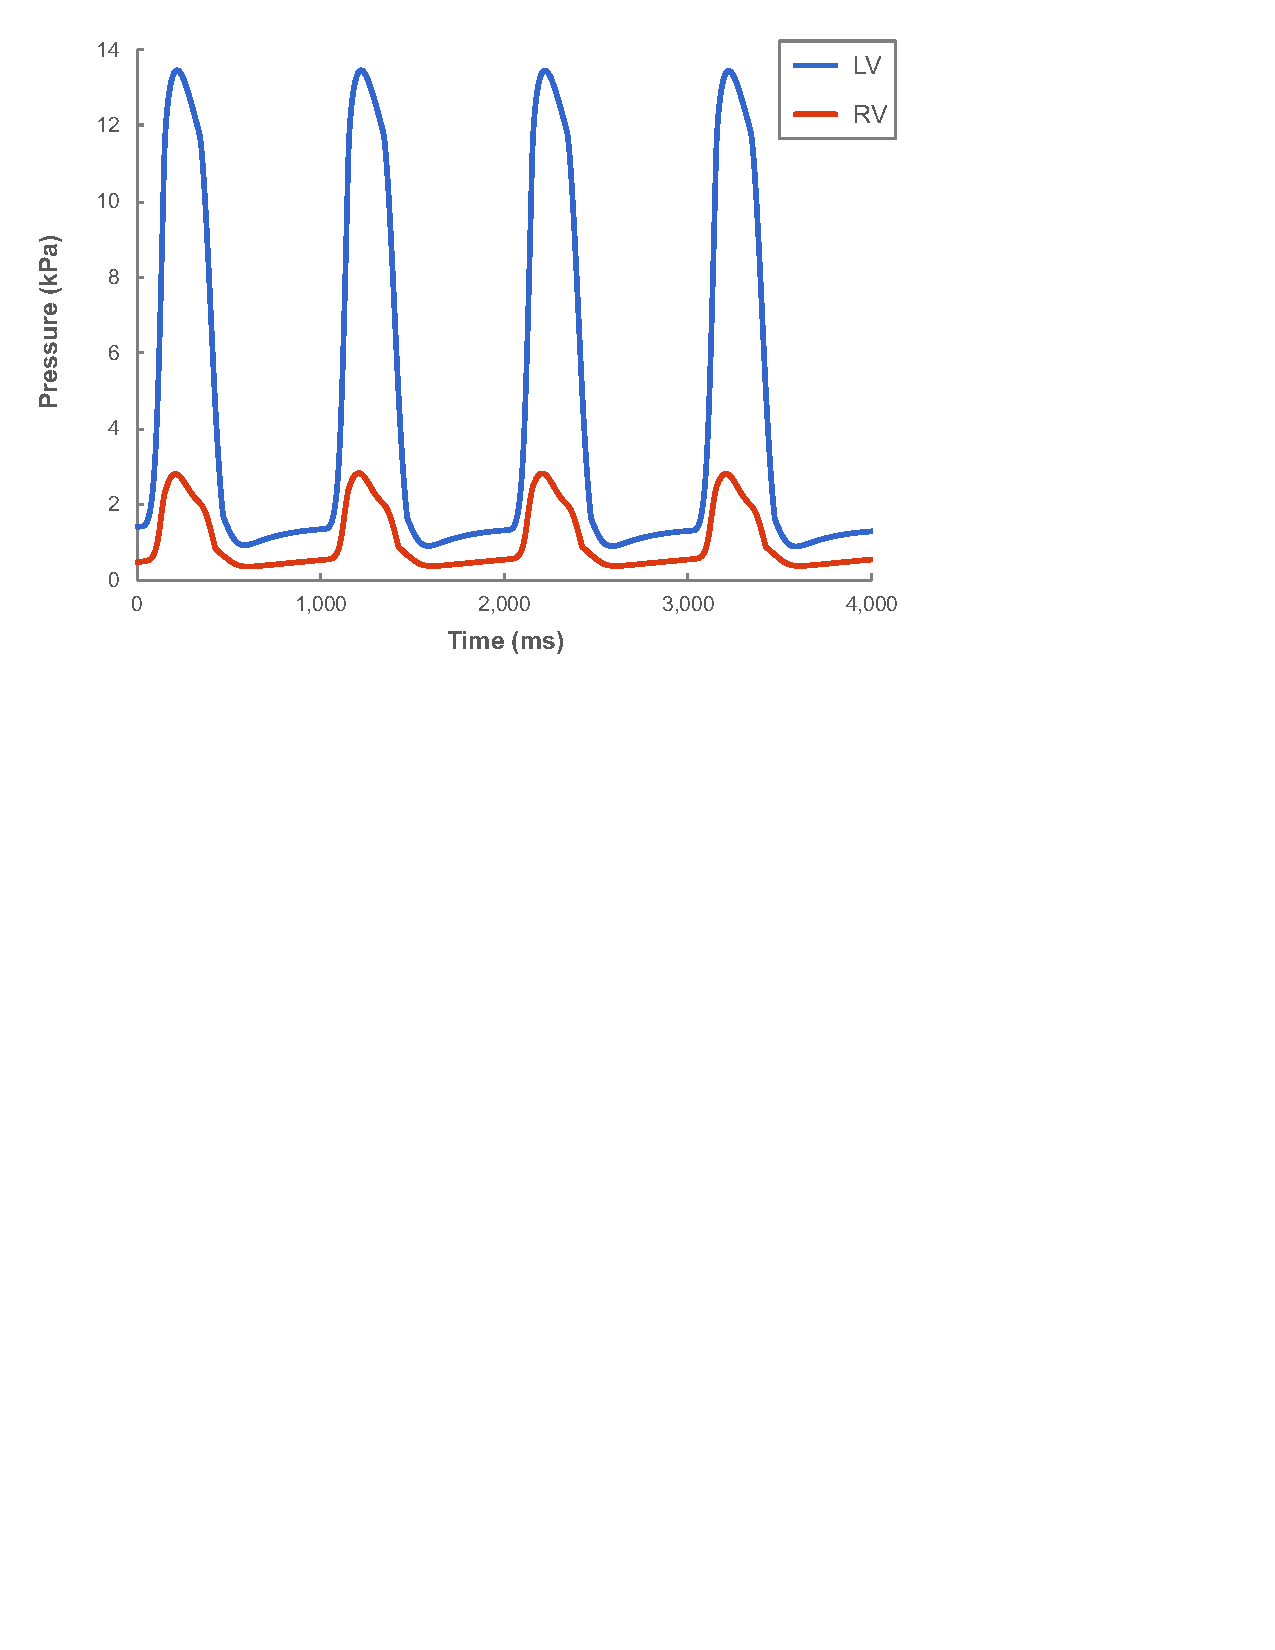
\includegraphics[scale=0.5]{media/4-cardioid/5-pv/pressure_volume-2.pdf}
\label{fig:pv2}}		
%
\caption{Results from Cardioid simulation: (a) P-V loop of left ventricle, (b) pressure time history in left and right ventricles.}
\label{fig:pv}
\end{figure}

\begin{figure}[ht!]
\centering
\subfigure[]{%
		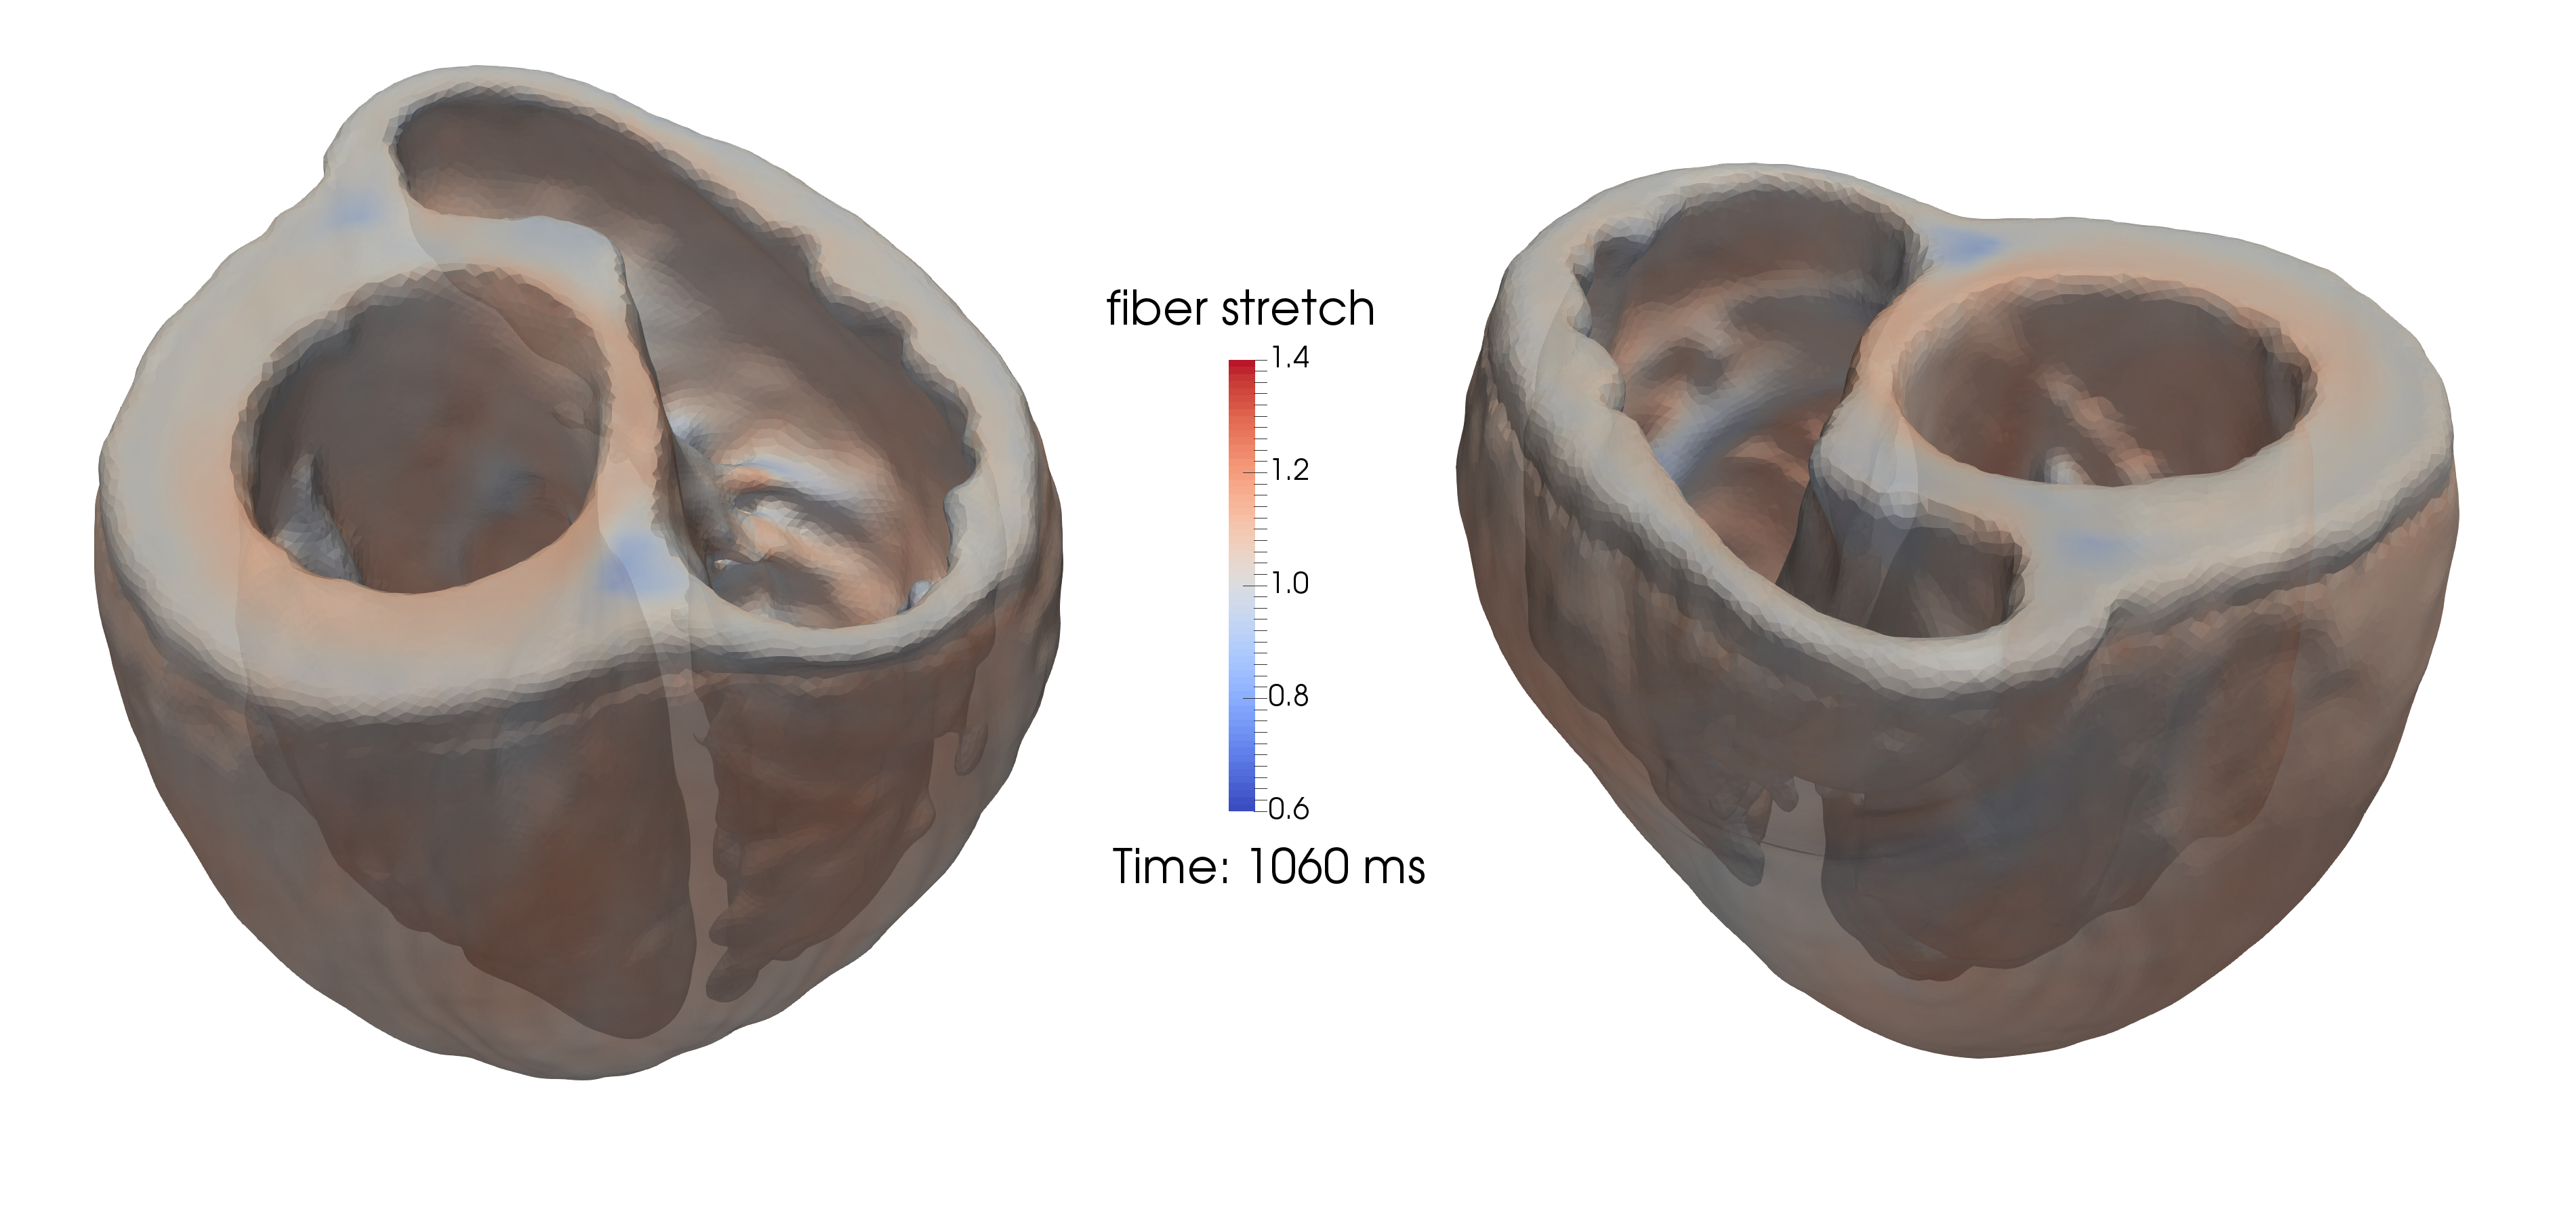
\includegraphics[scale=0.057]{media/4-cardioid/6-vid/a.png}
\label{fig:snaps1}}		
\subfigure[]{%
		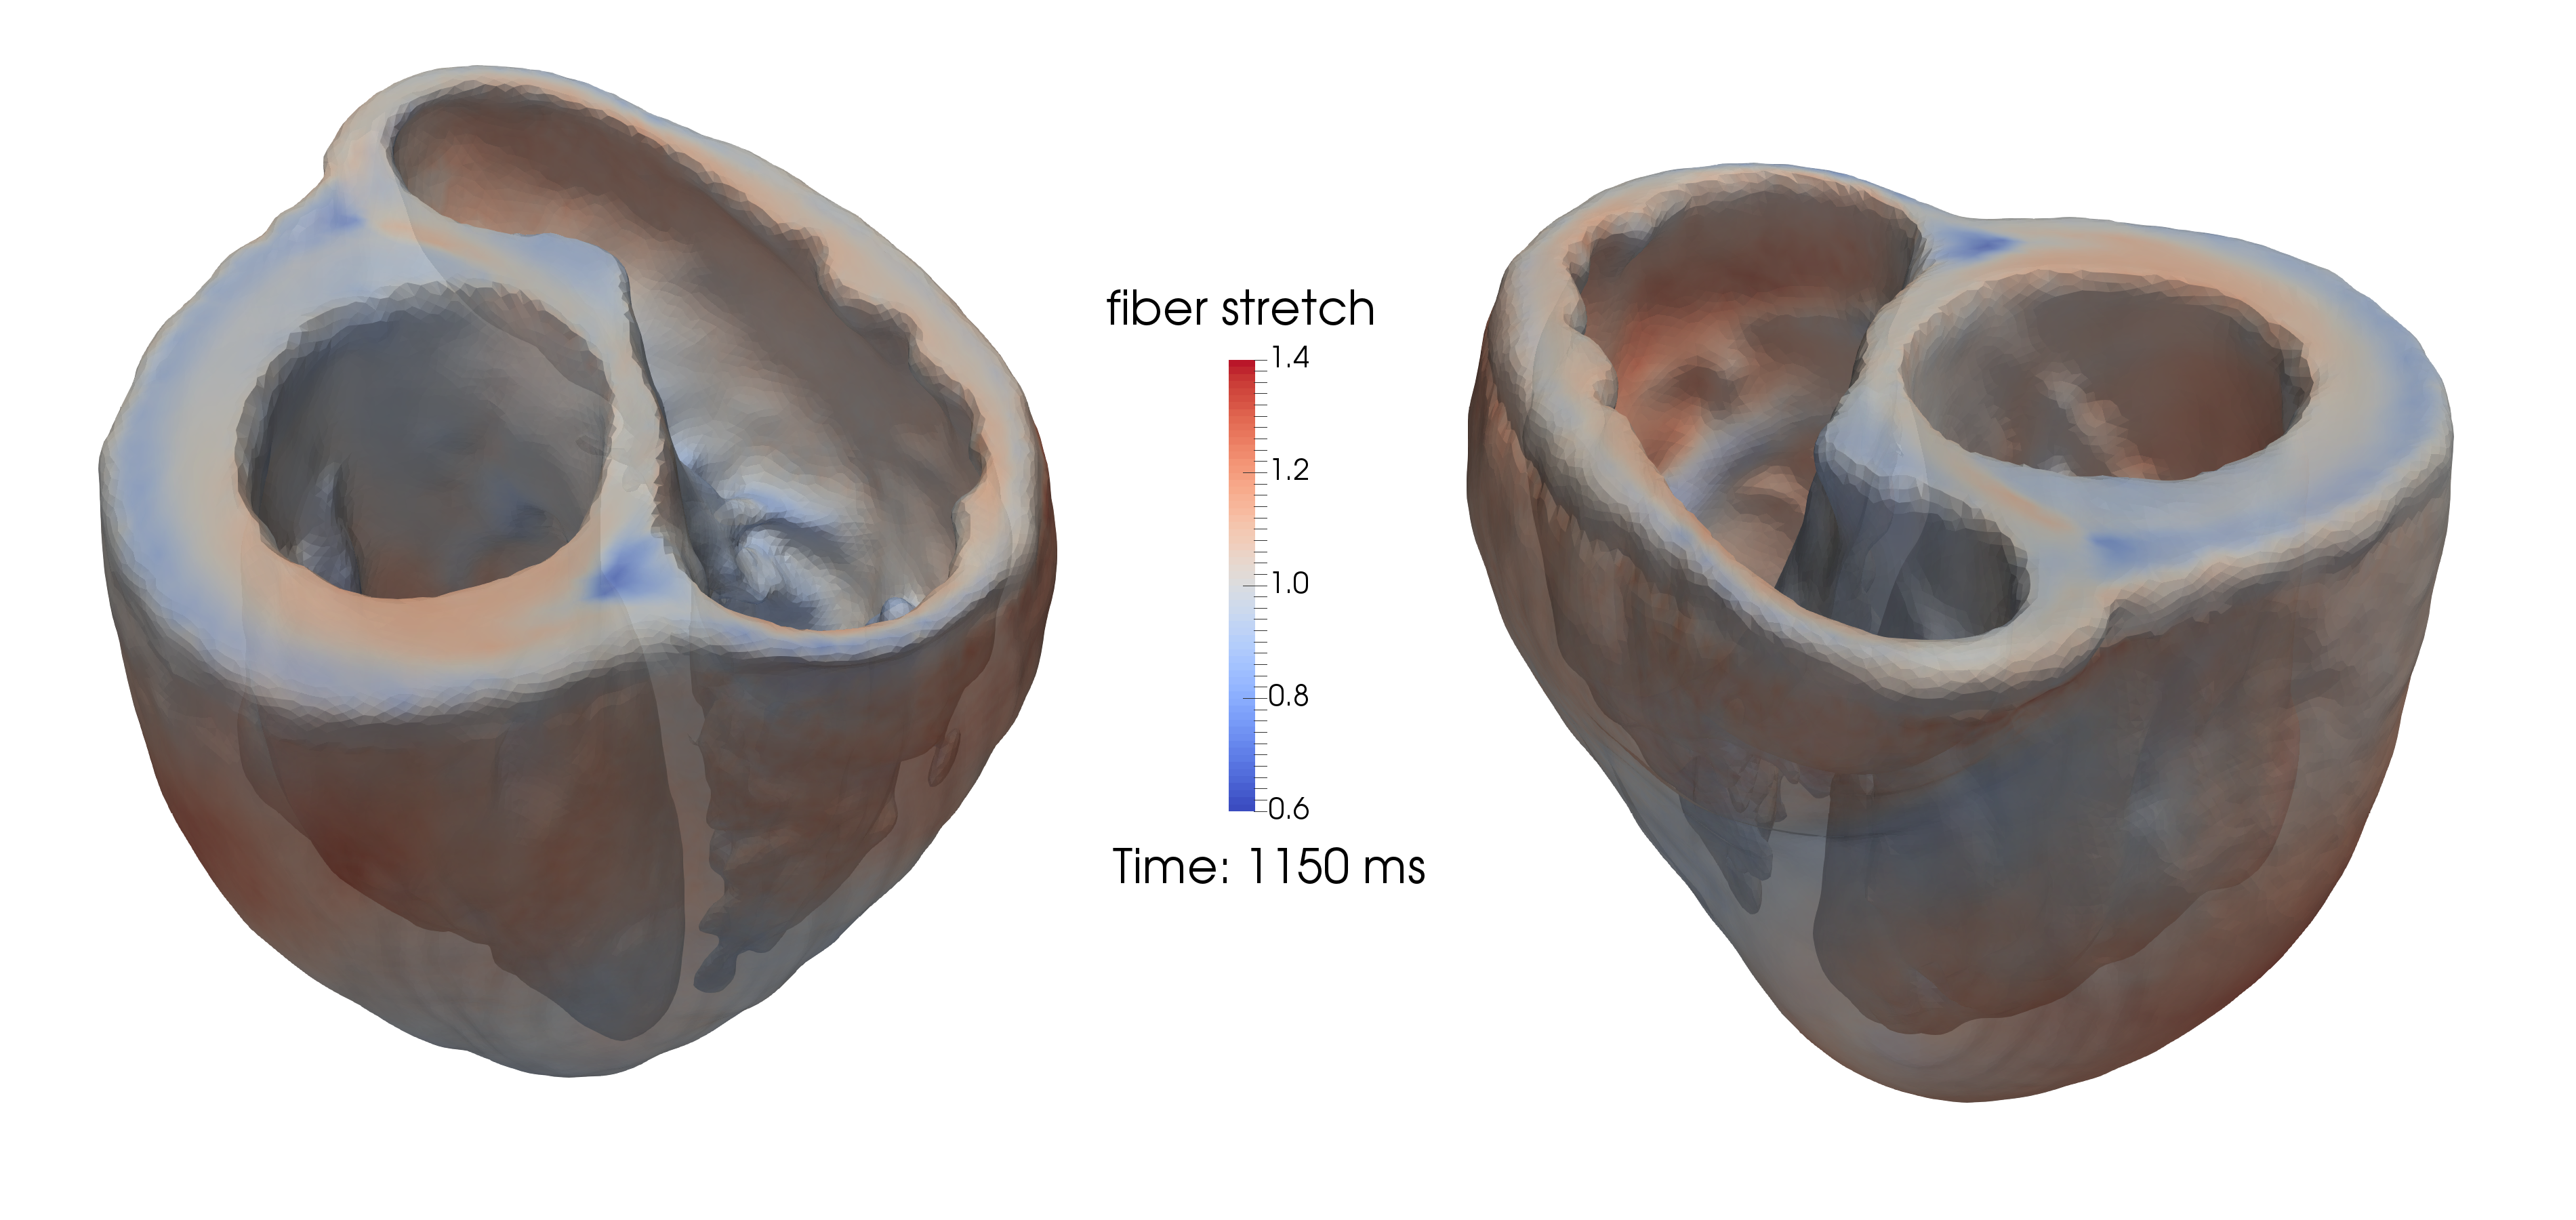
\includegraphics[scale=0.057]{media/4-cardioid/6-vid/b.png}
\label{fig:snaps2}}		
\subfigure[]{%
		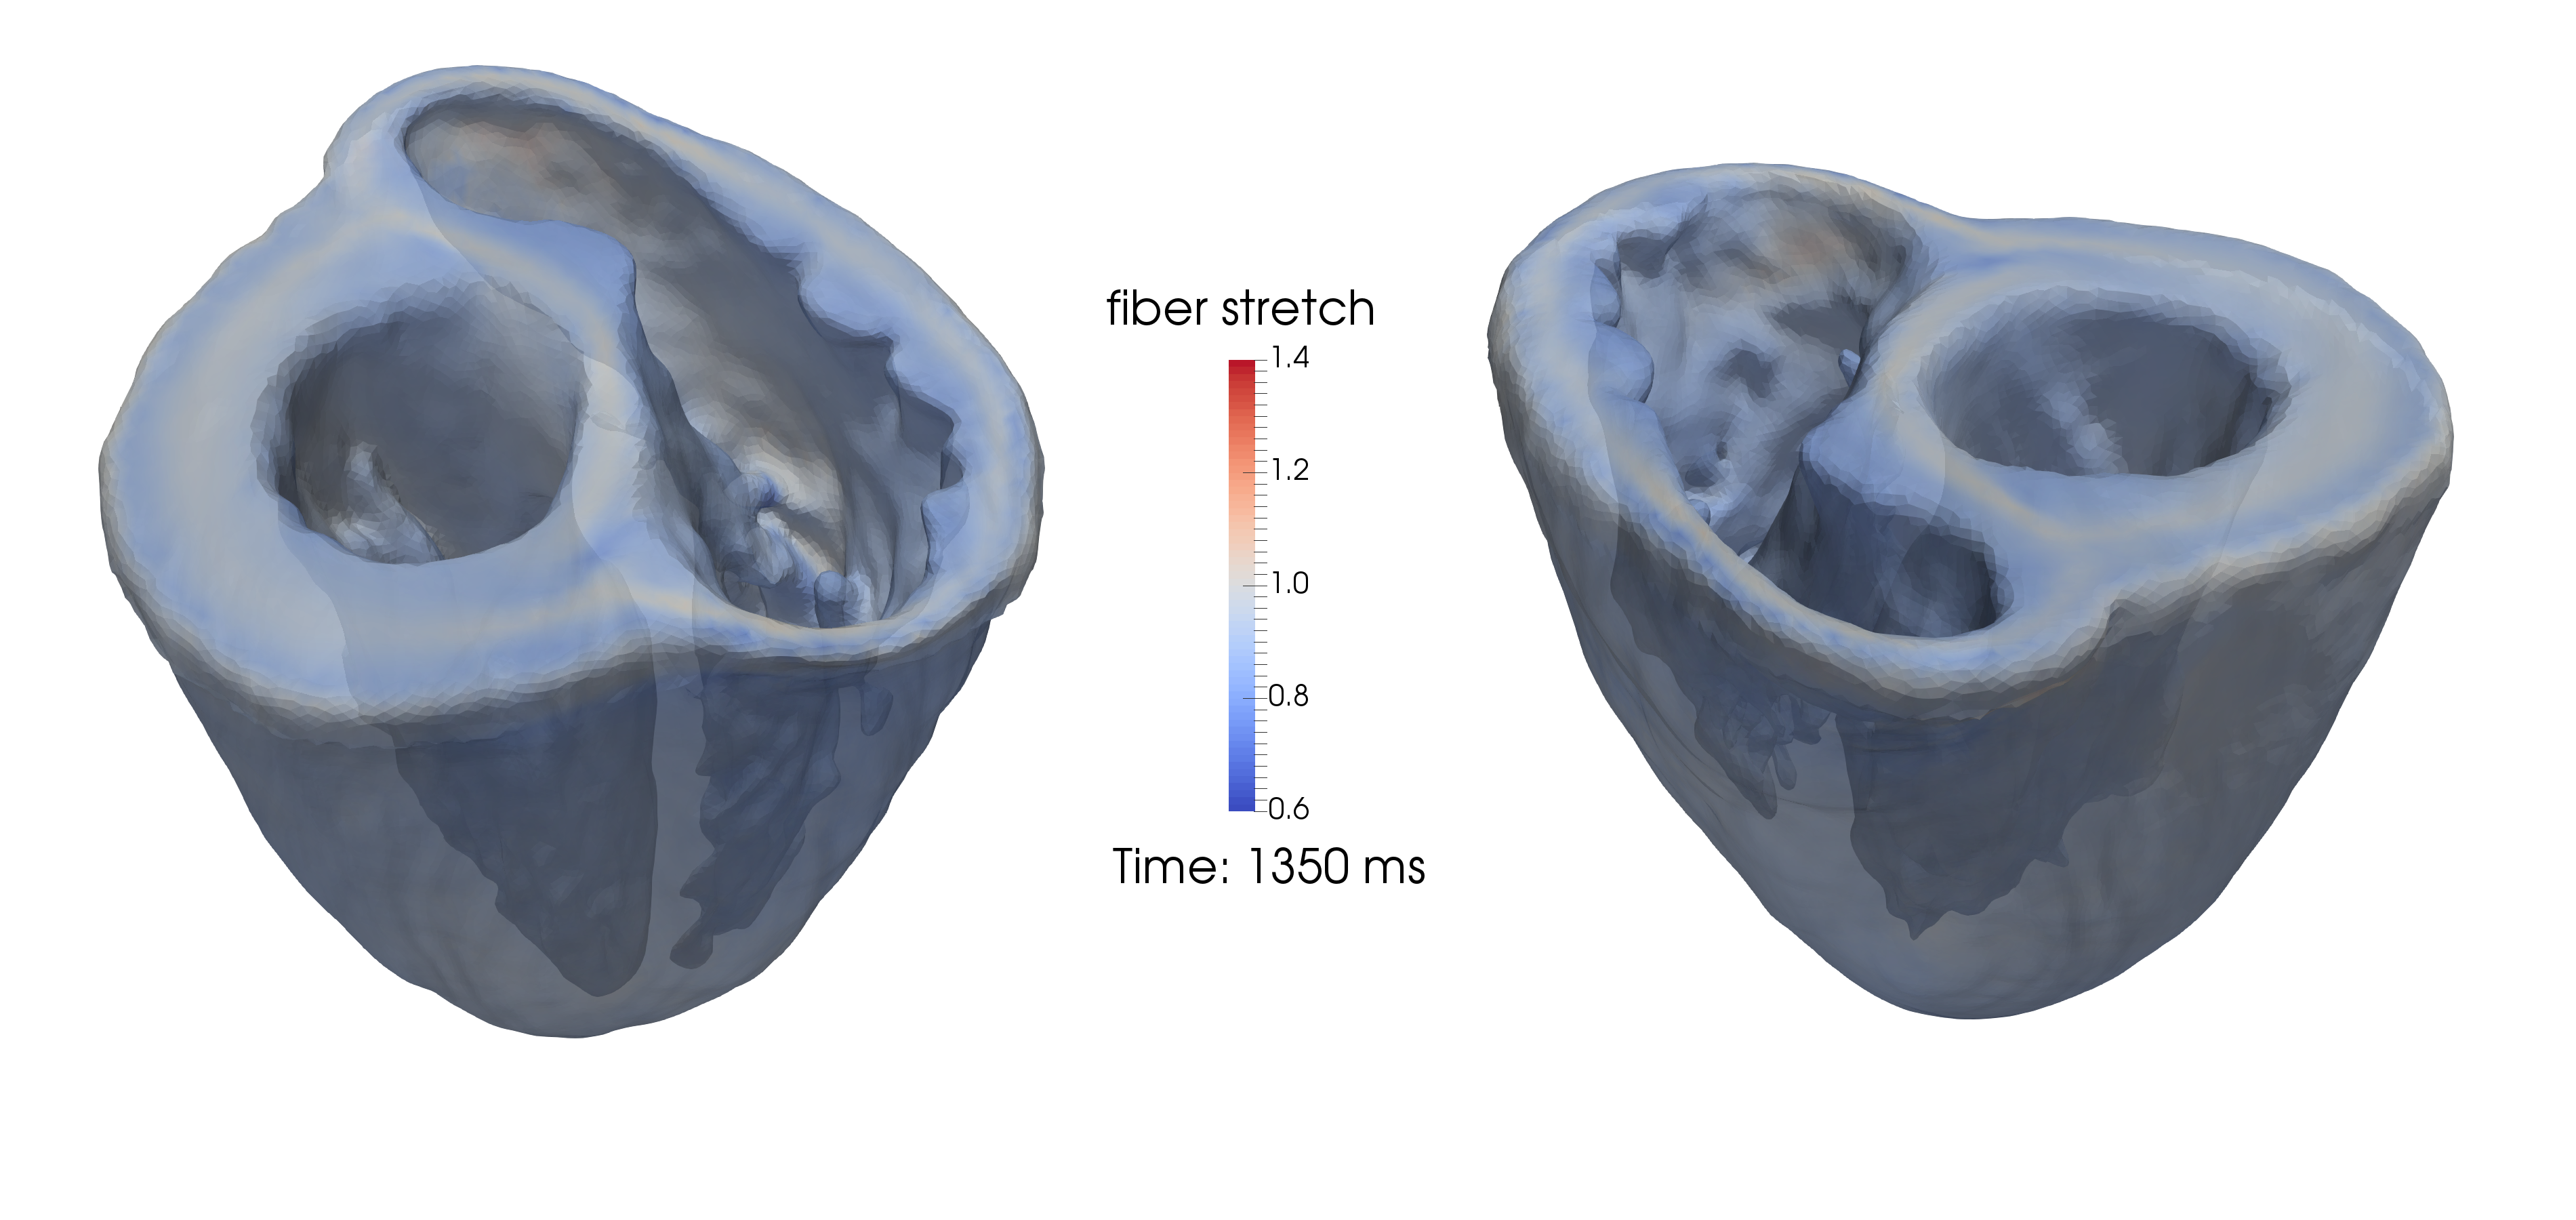
\includegraphics[scale=0.057]{media/4-cardioid/6-vid/c.png}
\label{fig:snapsf3}}		
\subfigure[]{%
		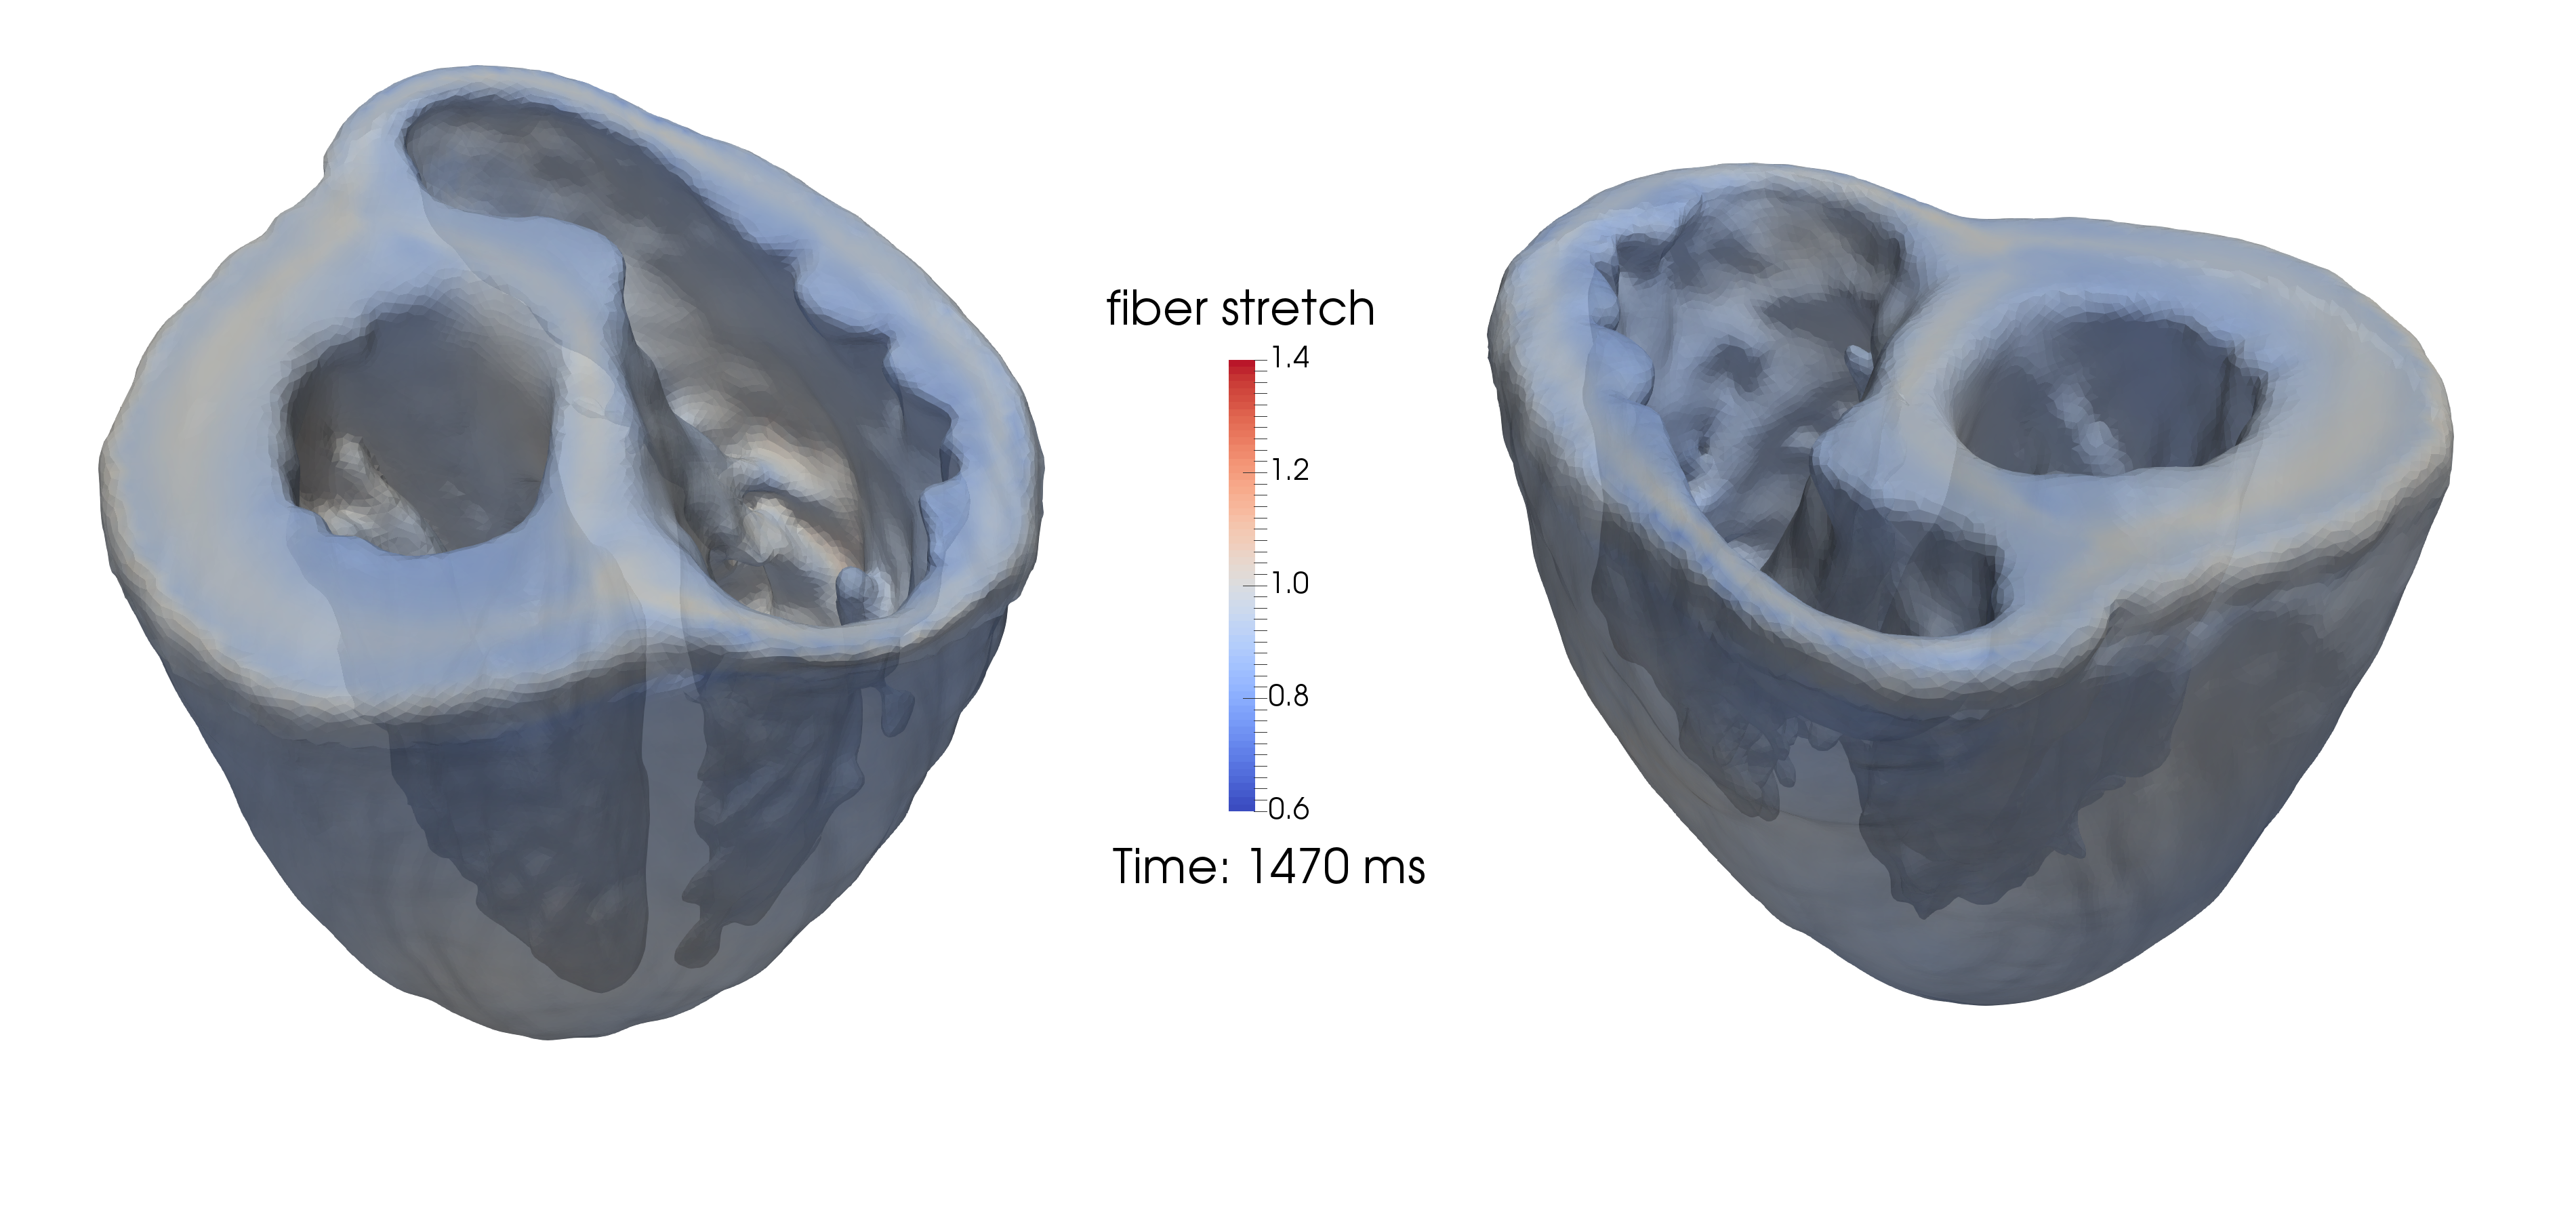
\includegraphics[scale=0.057]{media/4-cardioid/6-vid/d.png}
\label{fig:snaps4}}		
%
\caption{Deformed mesh from Cardioid simulation at different stages of cardiac cycle. Panels (a), (b), (c), and (d) correspond to the stages in the P-V loop denoted in~\figref{pv}.}
\label{fig:snaps}
\end{figure}

%%%%%%%%%%%%%%%%%%%%%%%%%%%%%%%%%%%%%%%%%%%%%%%
%%%%%%%%%%%%%%%%%%%%%%%%%%%%%%%%%%%%%%%%%%%%%%%
\section{Extension to Polyhedral Finite Elements}
\label{Polyhedral Finite Elements}

Efforts have been made to implement the mechanics described in this chapter into the polyhedral FEM code \textit{Celeris}. The details of the implementation will be discussed, followed by an expos\'{e} of cardiac verification problems using polyhedral finite elements.

\subsection{Implementation}

The same surface mesh used to produce the quadratic tetrahedral mesh for Cardioid is used to produce the polyhedral mesh in Celeris shown in \figref{compdof} and \figref{cel}. The Usyk material model is implemented within the Celeris framework. Rather than full incompressibility via a mixed displacement-pressure formulation, near-incompressibility is enforced via 1) a penalty term in the strain energy for volumetric material response, together with 2) an F-bar projection method. Regarding the penalty term, the strain energy is defined in the following manner, as is done by Usyk\textit{et al.}~\cite{usyk_2002}:
\begin{equation}
W = \frac{C}{2}\left(e^Q -1\right) + C_{compr} (J \cdot \ln J - J + 1) \\
\end{equation}
The parameter $C_{compr}$ is a penalty parameter, such that the volumetric response of the material is significantly stiffer than the deviatoric response. It was found that a value of $C_{compr} \geq 200  C$ gives good results compared to those when enforcing full incompressibility through a mixed pressure-displacement formulation, without significantly making the system poorly conditioned. Interestingly, the value of $C_{compr}$ provided by Usyk \textit{et al.} is actually not nearly large enough to produce results that are competitive with fully incompressible formulations.

%%%%%%%%%%%%%%%%%%%%%%%%%%%%%%%%%%%%%%%%%%%%%%%%%%%%%%%%
%%%%%%%%%%%%%%%%%%%%%%%%%%%%%%%%%%%%%%%%%%%%%%%%%%%%%%%%

Near-incompressibility is enforced by an F-bar projection method, in which the deformation gradient is modified such that the dilatation $e = \text{tr}(\nabla{u})$ at each integration point is replaced by an element-averaged value. Specifically, the deformation gradient at each integration point is redefined as:
\begin{align}
\tilde{\bm{F}}_i = \alpha_i\bm{F}_i \\
\tilde{e}_i = \Sigma_k e_k
\end{align}
where $\alpha_i$ is the coefficient that modifies the deformation gradient $\bm{F}_i$ at the $i$th integration point, such that the dilatation $e_i$ becomes the average over the $k$ integration points in the particular element, while the deviatoric portion of $\bm{F}_i$ is untouched. Specifically, the deviatoric portions of $\tilde{\bm{F}}$ remain $\bm{F}$ are equal.
~~~
cite f-bar projection
look at imitor code and Mark notes
~~~

The material model framework in Celeris currently accepts material model definitions in \textit{incremental form}, namely, the material model takes as input the material properties and other field parameters, the beginning step stress $\overline{\bm{T}}$, beginning step state variables $\overline{bm{q}}$, and strain rate $\bm{D}$, and produces as output an end step stress $\bm{T}$, end step state variables $\bm{q}$, and end step tangent modulus $\frac{\partial \bm{T}}{\partial \bm{D}}$. Hyperelastic materials are generally defined as functions of the deformation gradient $\bm{F}$, though, not of the strain rate $\bm{D}$. Thus, a deformation path from beginning step to end step is assumed in the following manner, as is done by Rashid~\cite{}:
\begin{equation}
blah
\end{equation}
whose solution is 

The beginning step deformation gradient is stored as a state variable to accommodate the incremental material form, initialized as the identity tensor and updated within each call to the material model as $\bm{F} \leftarrow \hat{\bm{U}}\bm{F}$. Field parameters at each integration point include: the fiber transformation matrix $\bm{Q}$, activation time $t_a$. Finally the material model also admits the fixed beat duration, as well as the beginning and end step times - quantities used in the calculation of active tension. The fiber transformation matrix $\bm{Q}$ and activation time $t_a$ are computed via Cardioid \textit{a priori} and are imported into Celeris at the integration points.

%%
% DESCRIBE ENTIRE PROCESS
%%

%
% COMMENTS ON ACTIVE PORTION
%
For this particular implementation, the fiber orientations in \eqnref{active} are taken to be in the \textit{current} configuration (AS AN IMPROVEMENT). The Fortran code for the model is produced by the LLNL tool \textit{Melodee}, a new language for expressing systems of ODEs that generates optimized code at runtime for different platforms. Melodee was tested and verified to generate working Fortran subroutines. The tangent modulus corresponding to the active portion of stress was computed and verified, although no rigorous verification of the model to produce expected active stress values has been performed yet.

Finally, as discussed in \chapref{4}, the end step stress is forward rotated via $\bm{R}^T \bm{T} \bm{R}$ and the state variable $\bm{F}$ is forward rotated simply via $\bm{R}\bm{F}$.

The passive material model has been implemented, and the computed stress and corresponding tangent modulus have been thoroughly verified against finite difference approximations for accurate and quickly converging solutions.

%%%%%%%%%%%%%%%%%%%%%%%%%%%%%%%%%%%%%%%%%%%%%%%%%%%%%%%%
%%%%%%%%%%%%%%%%%%%%%%%%%%%%%%%%%%%%%%%%%%%%%%%%%%%%%%%%

The same Dirichlet boundary conditions applied in Cardioid are applied in Celeris using the same surface tags shown in \figref{supp3}. For simplicity, the ventricular pressure time histories from the Cardioid simulation is used directly for the imposition of ventricular boundary conditions in Celeris, rather than imposing volume constraints as described previously. Of course, in the future the volume constraint would be implemented as well so that the Celeris mechanics is completely independent of the Cardioid mechanics. The pressure time histories $p_{LV}(t)$ and $p_{RV}(t)$ are enough to demonstrate the workflow using polyhedral FEM and highlighting the advantages of PEM over conventional FEM.

\subsection{Verification}

Prior to running a complete cardiac simulation, the polyhedral workflow was tested for a suite of verification problems. Six verification problems were identified: three from Gurev \textit{et al.}~\cite{gurev_2015} and three from Land \textit{et al.}~\cite{land_2015}. The specifics of those problems can be found in the those papers. See \figref{beams} and \figref{ventricles} for the nomenclature used to identify the problems, as well as the type of mechanics being tested for each one.

\begin{figure}[ht]
\centering
\subfigure[]{%
		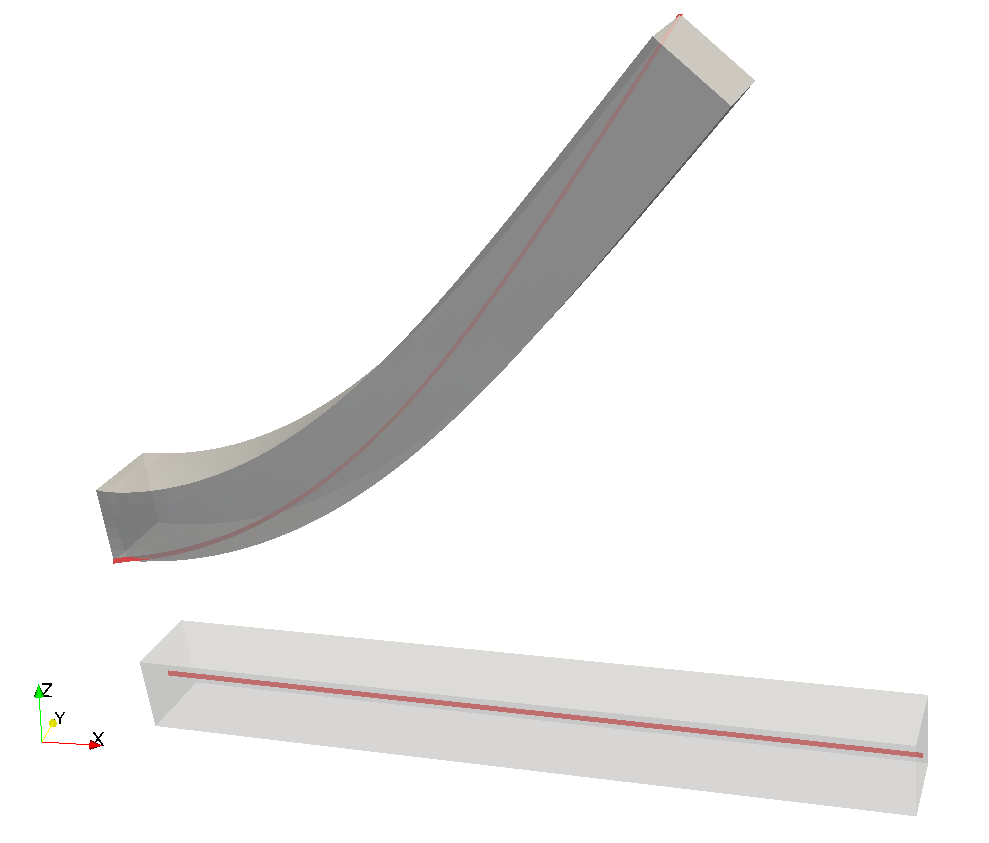
\includegraphics[scale=0.18]{media/5-verif/1-gurev2/gurev2.png}
\label{fig:beams1}}		
\subfigure[]{%
		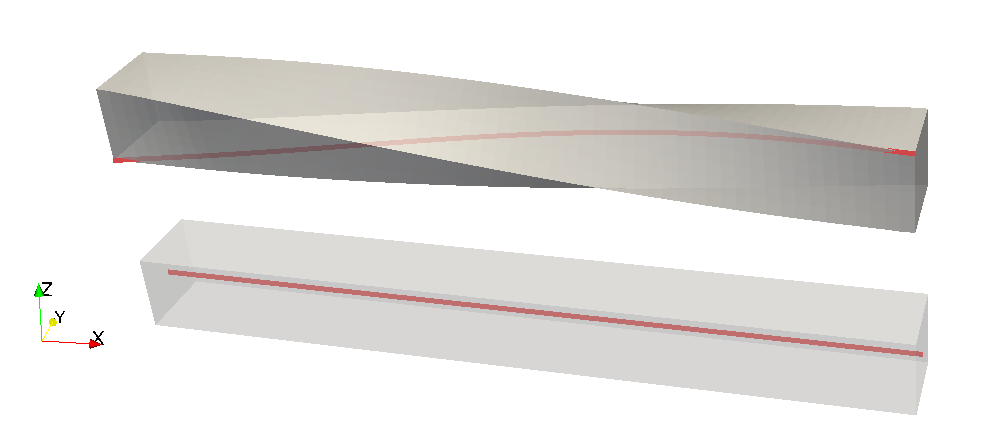
\includegraphics[scale=0.18]{media/5-verif/2-gurev3/gurev3.png}
\label{fig:beams2}}		
\subfigure[]{%
		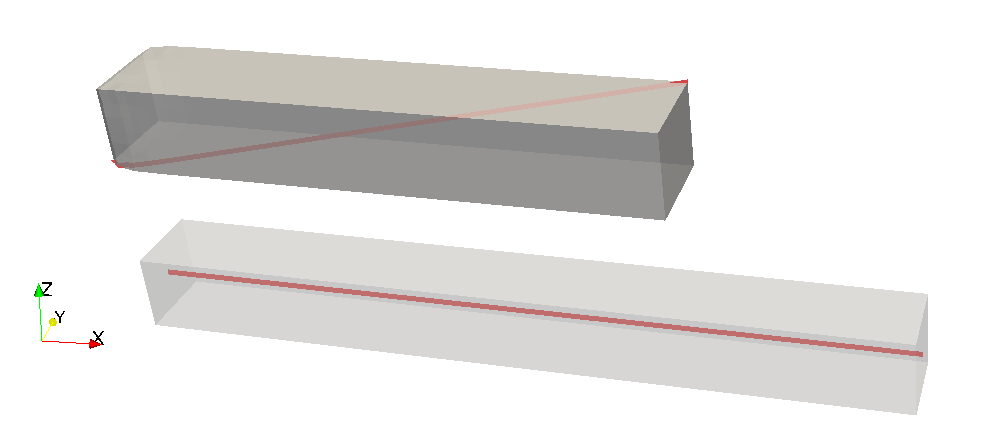
\includegraphics[scale=0.18]{media/5-verif/3-gurev4/gurev4.png}
\label{fig:beams3}}		
\subfigure[]{%
		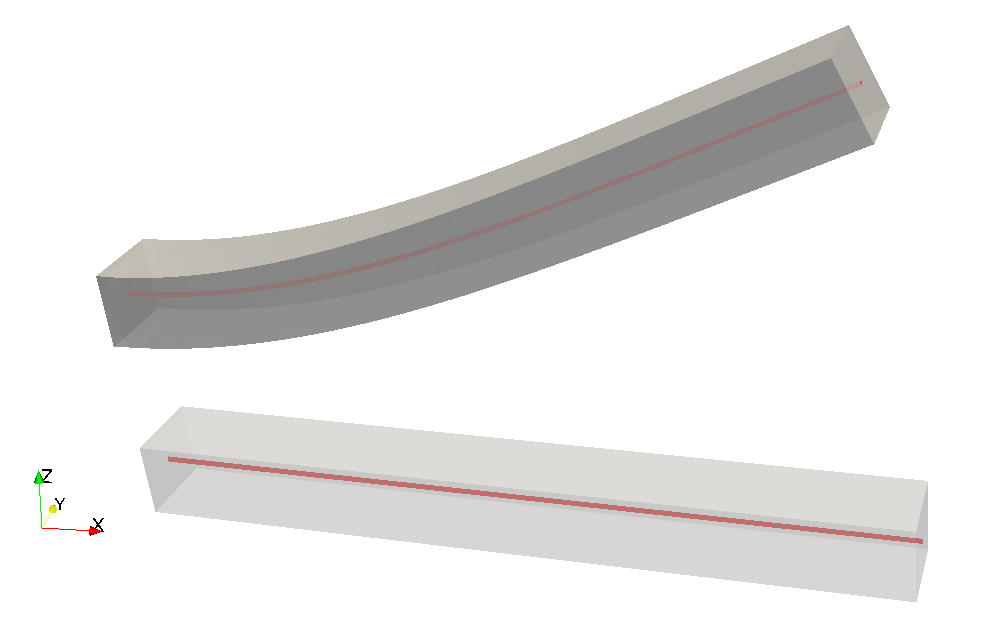
\includegraphics[scale=0.18]{media/5-verif/4-land1/land1.png}
\label{fig:beams4}}		
%
\caption{Undeformed (bottom) and deformed (top) configurations for cantilever beam verification problems: (a) Gurev P2: bending, (b) Gurev P3: torsion, c) Gurev P4: active contraction, and (d) Land P1: bending. The red curve denotes the curve over which displacements and positions are recorded and compared.}
\label{fig:beams}
\end{figure}

\begin{figure}[ht]
\centering
\subfigure[]{%
		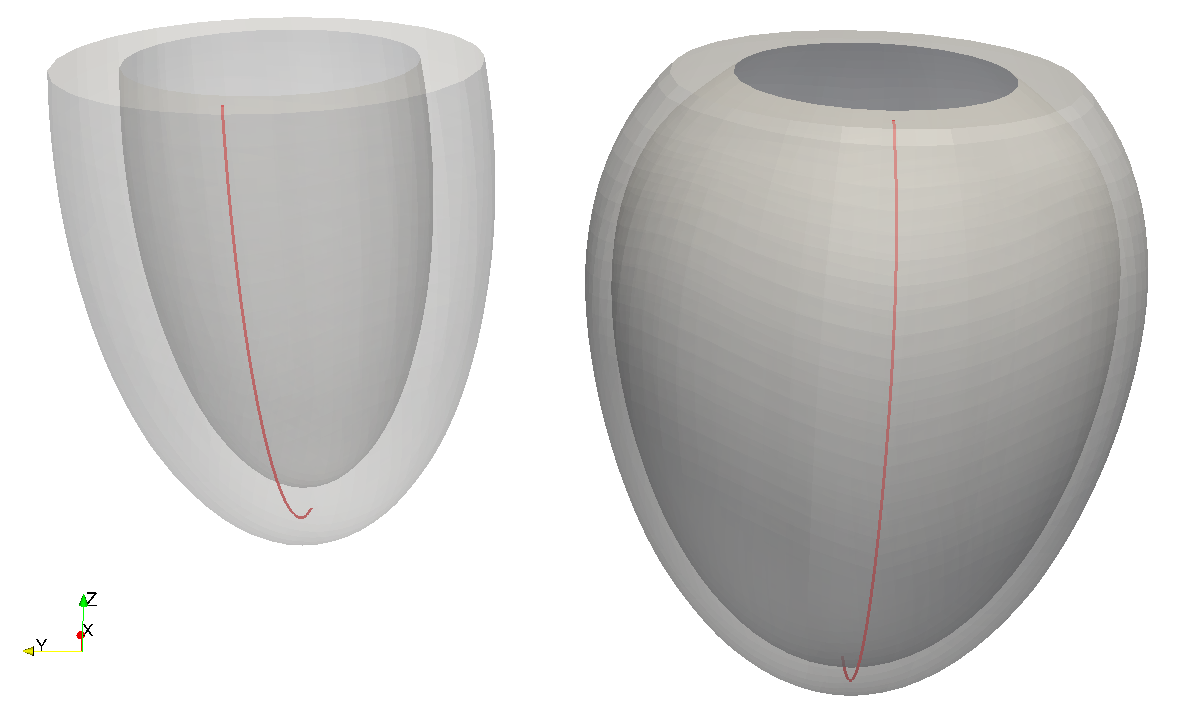
\includegraphics[scale=0.18]{media/5-verif/5-land2/land2-1.png}
\label{fig:ventricles1}}		
\subfigure[]{%
		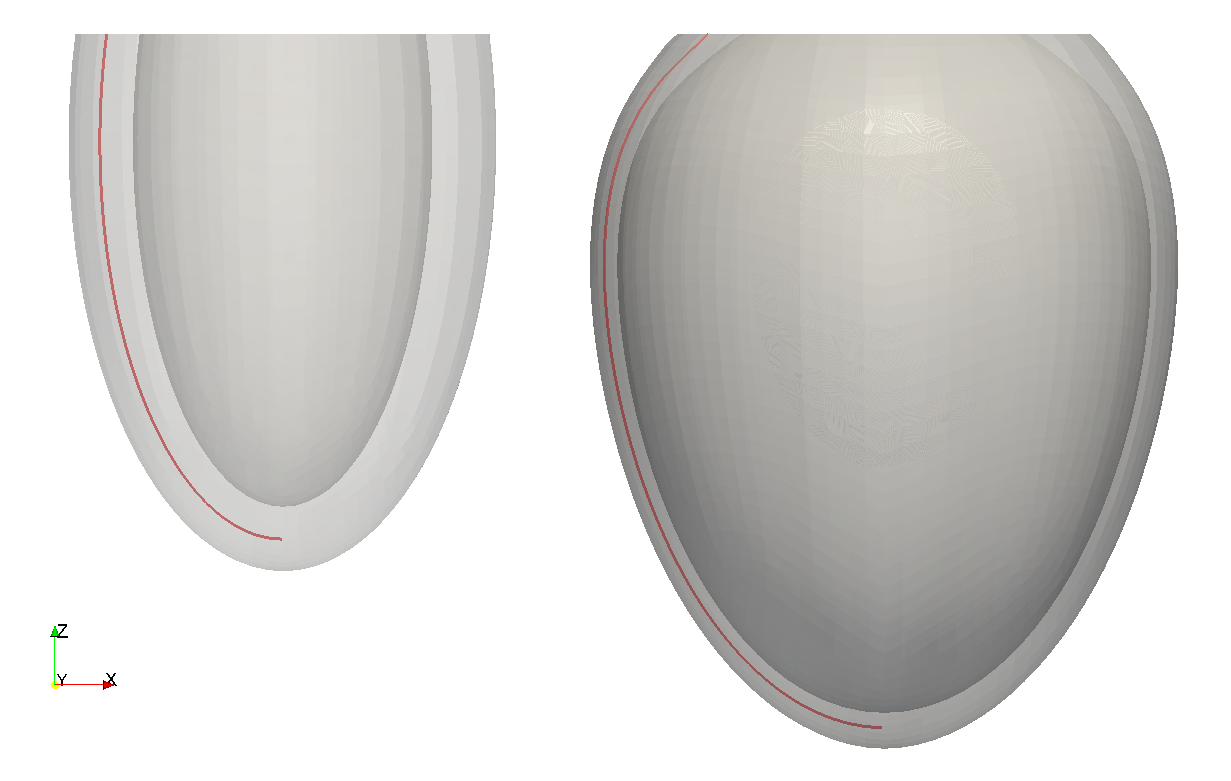
\includegraphics[scale=0.18]{media/5-verif/5-land2/land2-2.png}
\label{fig:ventricles2}}		
\subfigure[]{%
		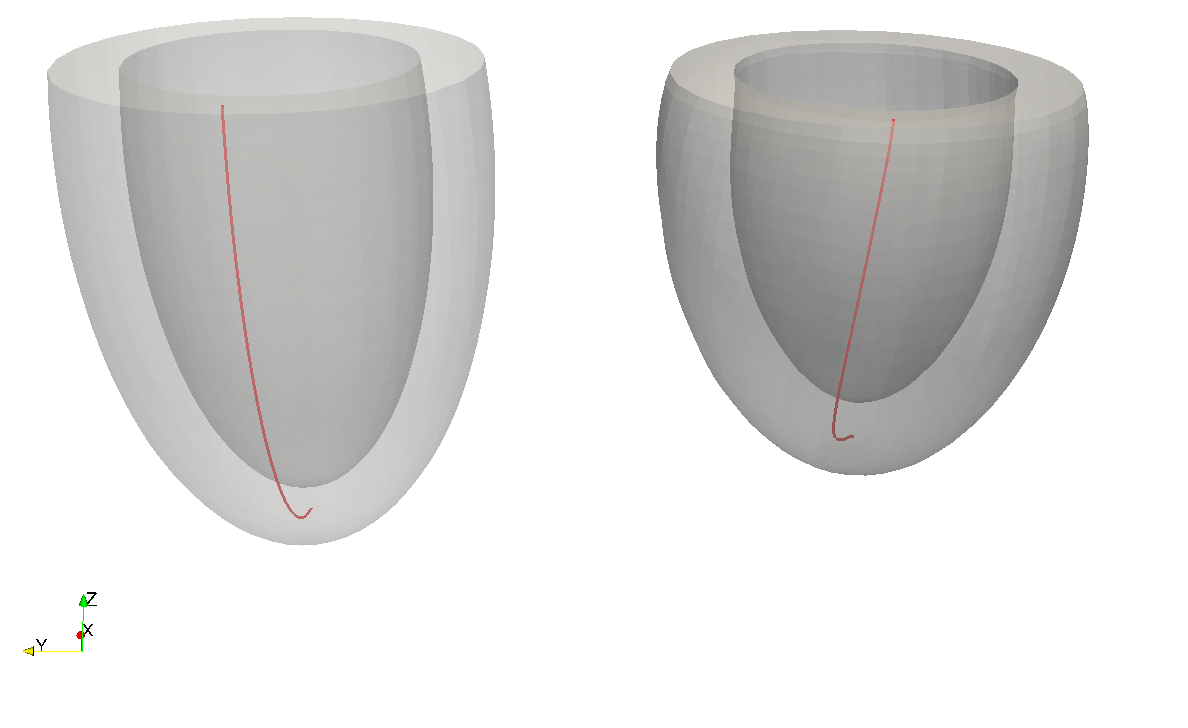
\includegraphics[scale=0.18]{media/5-verif/6-land3/land3-1.png}
\label{fig:ventricles3}}		
\subfigure[]{%
		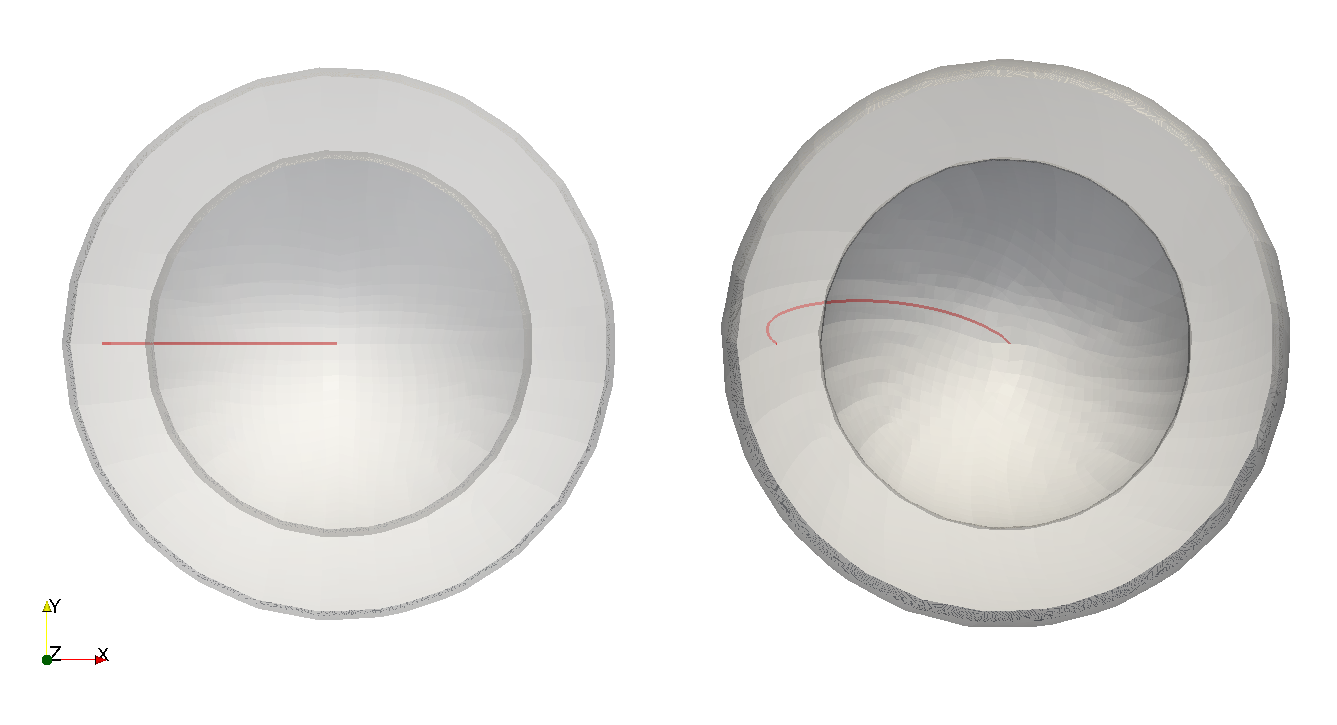
\includegraphics[scale=0.16]{media/5-verif/6-land3/land3-2.png}
\label{fig:ventricles4}}		
%
\caption{Undeformed (left) and deformed (right) configurations for single ventricle verification problems: (a,b) Land P2: inflation, and (c,d) Land P3: inflation and active contraction. The red curve denotes the curve over which displacements and positions are recorded and compared.}
\label{fig:ventricles}
\end{figure}

Figures \ref*{fig:gurev2}-\ref*{fig:land3.2} show the results for the six verification problems, mimicking the format used in the papers from which they came. The results are presented using Cardioid, Celeris, and an in-house finite element code \textit{Imitor}. The implementation considerations are nearly identical for Imitor and Celeris. Thus, differences in results can be distinguished based on the finite element formulation vs. the implementation of material model, near incompressibility, and the like.

As the figures show, the polyhedral code Celeris performs very well for the cantilever beam verification problems involving bending, twist, and active contraction. The deformed meshes nearly identically match those from the conventional FEM codes. For those problems, hexahedral elements are employed for the conventional FEM codes, and cuboidal PEM elements are used in Celeris. Namely, the element shapes are the same, while the element formulations differ.

Interestingly, the near-incompressible approach appears to be slightly too stiff in bending, but slightly too compliant in purely volumetric deformations based on the results exhibited using Imitor. The over-stiffness in bending is evidenced in Gurev P2, Land P1, and Land P2, whereas the over-compliance in volumetric deformation is evidenced in Gurev P4 and Land P3. Overall though, these results provide confidence that the codes are working correctly. 

Running Celeris for the single ventricular problems Land P2 and Land P3 hinges on some fixes in the infrastructure of that code, unrelated to the scope of this project. It is the hope that once these fixes are made, the suite of verification problems can be completed for all three codes referenced. A comparison of the number of degrees of freedom for Land P1 is provided (\figref{land1-3}), but it is not particularly interesting because the meshes are already quite coarse, and automated linear hex meshing for a simple cantilever beam geometry is easily achievable. It is the hope that for Land P2 and Land P3, accurate results can be achieved using Celeris with a significant reduction in the number of DOF, as explained in \chapref{3}.

Up to this point, the mechanics have been verified to be implemented correctly in Imitor and Celeris, and cuboidal polyhedral elements are performing well for the cantilever beam problems. Completing the verification process would involve running Land P2 and Land P3 in Celeris, as well as potentially running the cantilever beam problems again in Celeris with non-cuboidal polyhedral elements - after which point Celeris would be ready to perform the same cardiac simulations presented using Cardioid.

\begin{figure}[ht]
\centering
\subfigure[]{%
		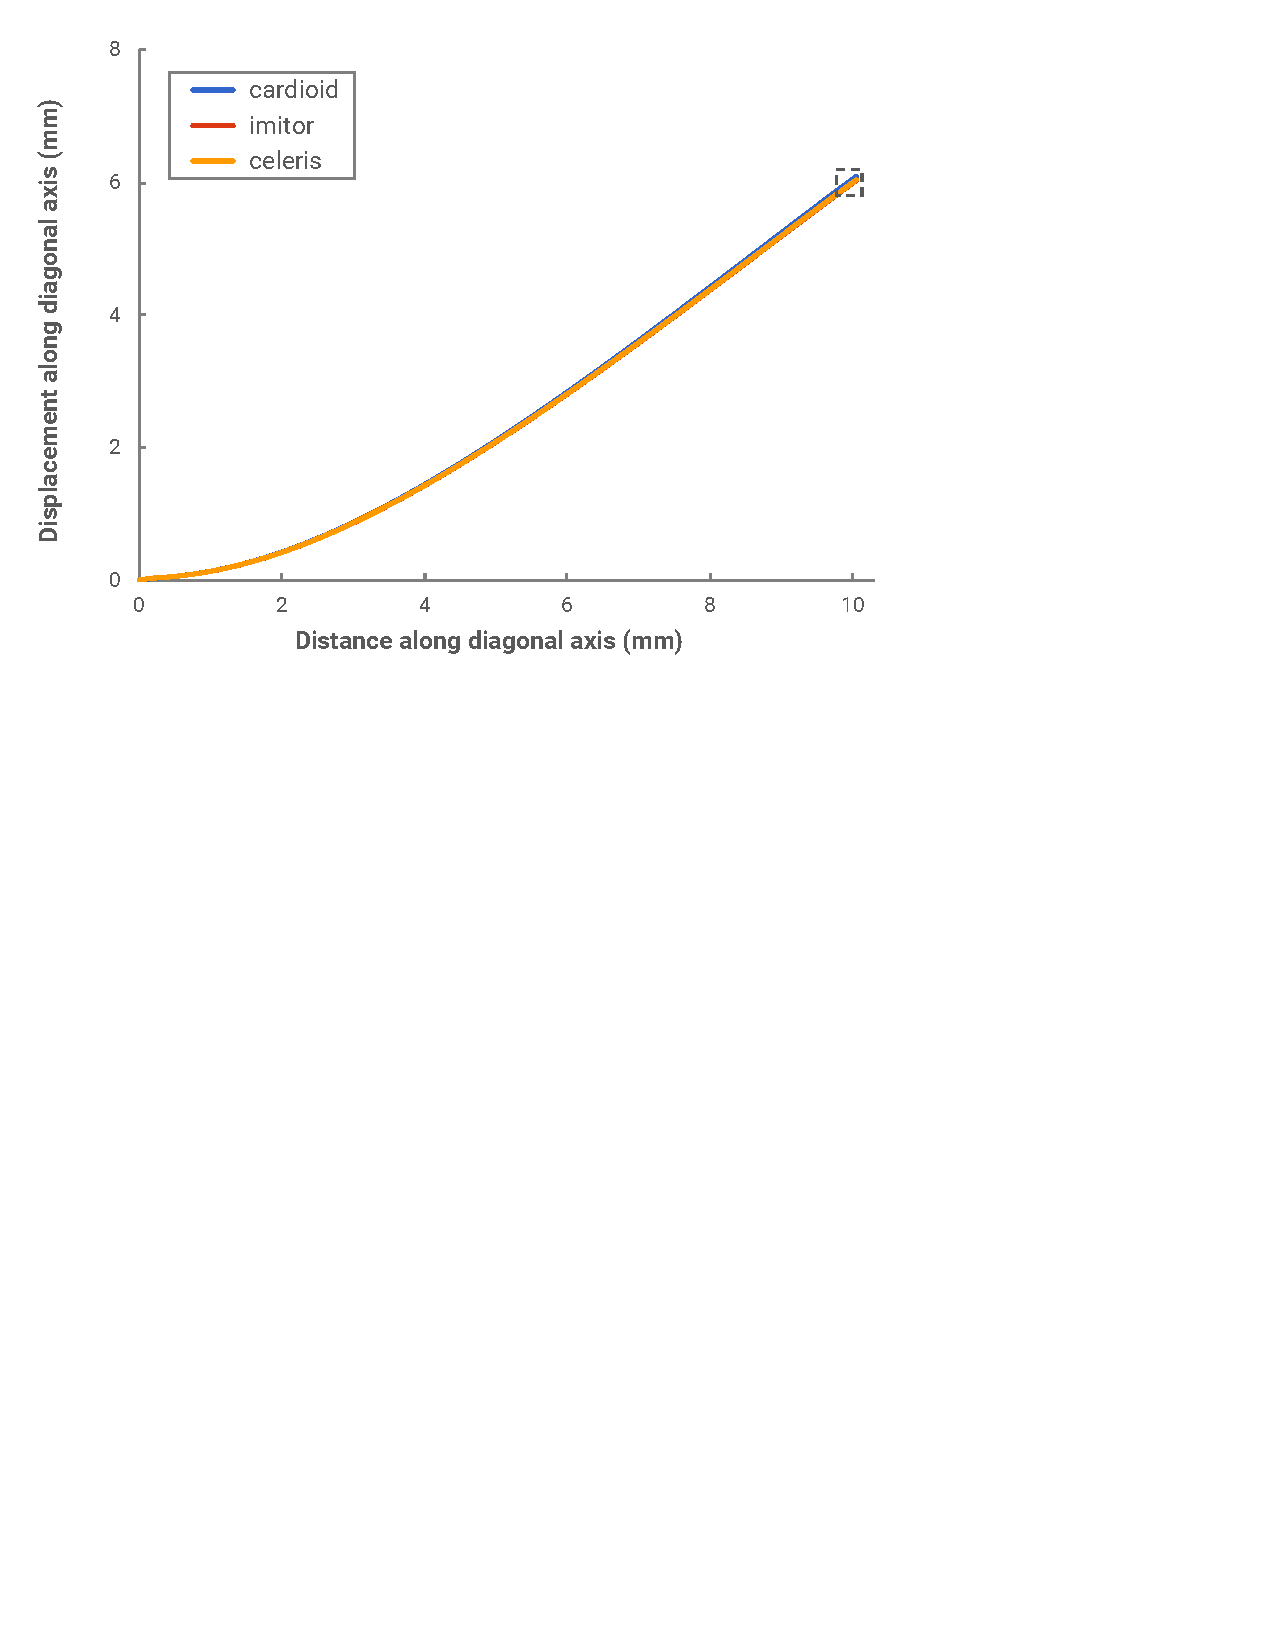
\includegraphics[scale=0.46]{media/5-verif/1-gurev2/gurev2-1.pdf}
\label{fig:gurev2-1}}		
\subfigure[]{%
		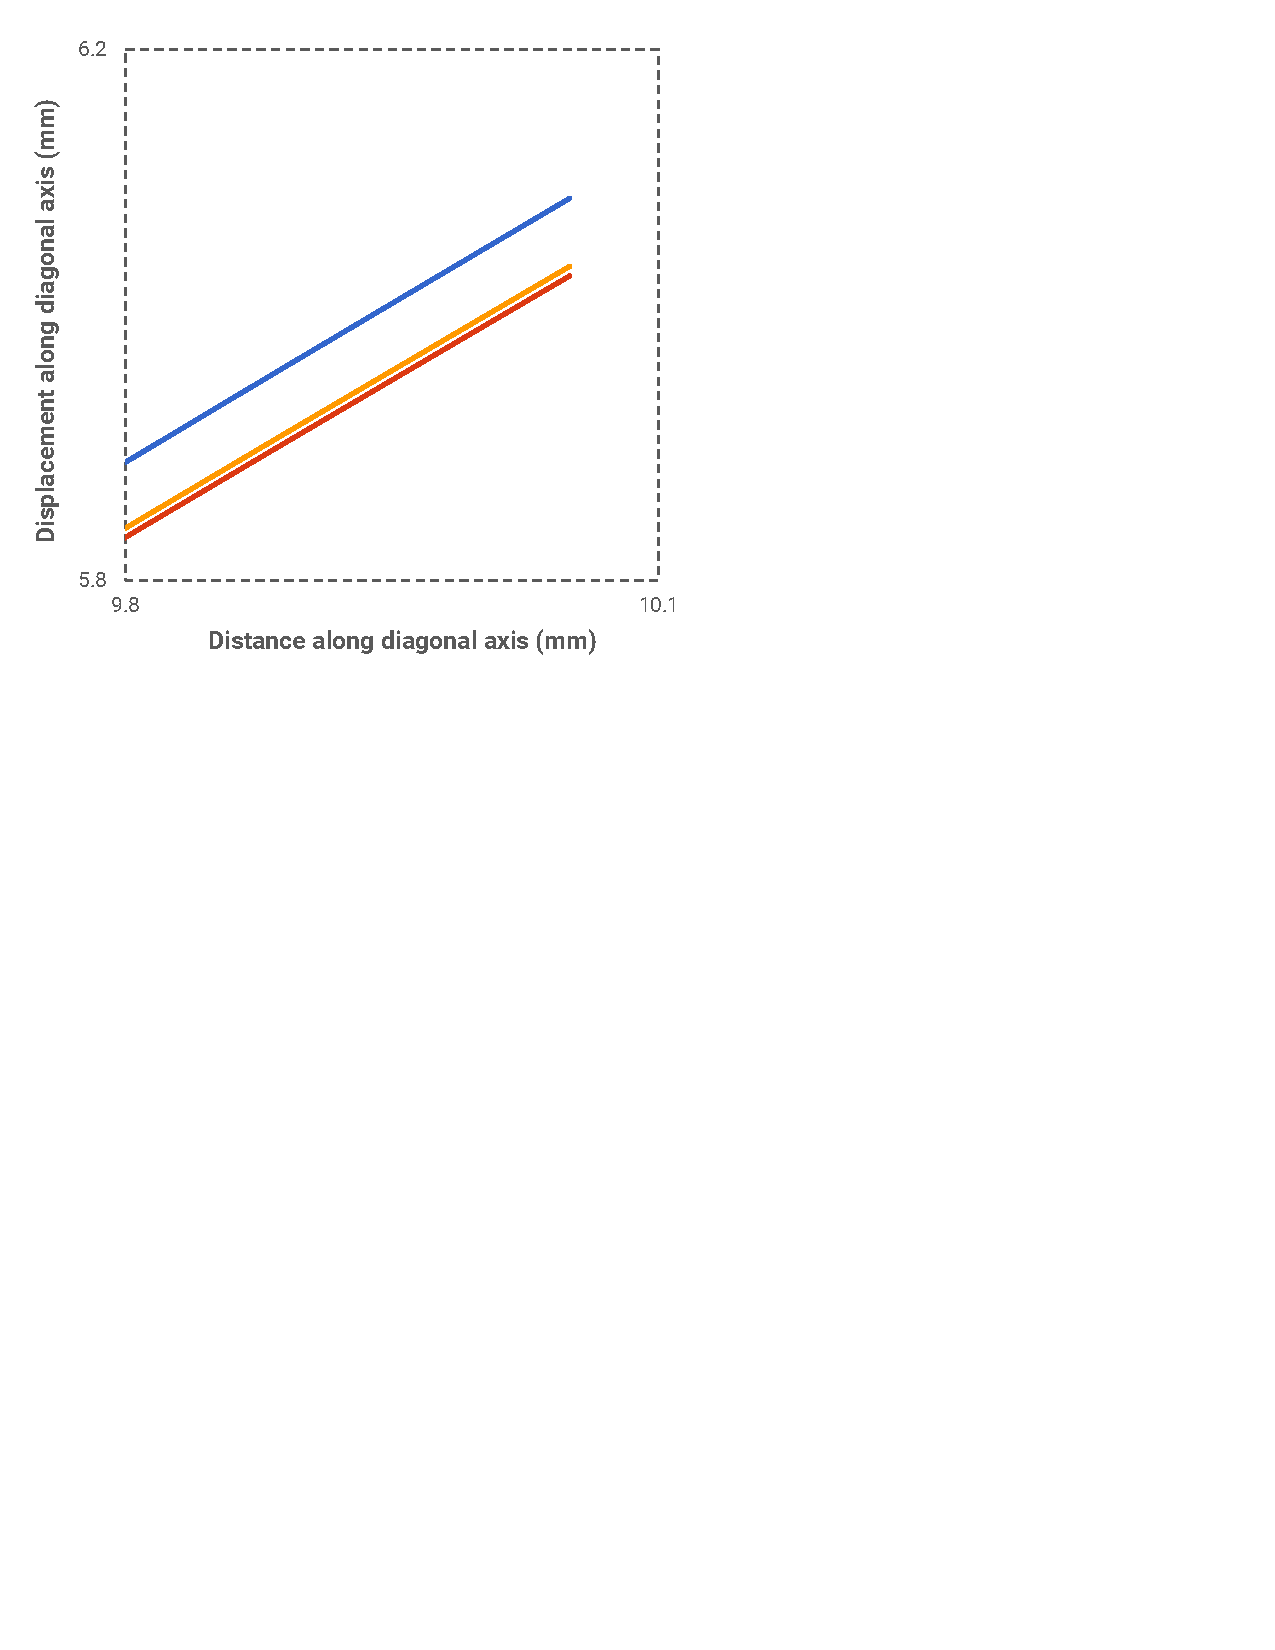
\includegraphics[scale=0.46]{media/5-verif/1-gurev2/gurev2-2.pdf}
\label{fig:gurev2-2}}		
%
\caption{Results for Gurev P2 verification problem: (a) Displacement magnitude along diagonal axis, with (b) details for the free end of the beam}
\label{fig:gurev2}
\end{figure}

\begin{figure}[ht!]
\centering
\subfigure[]{%
		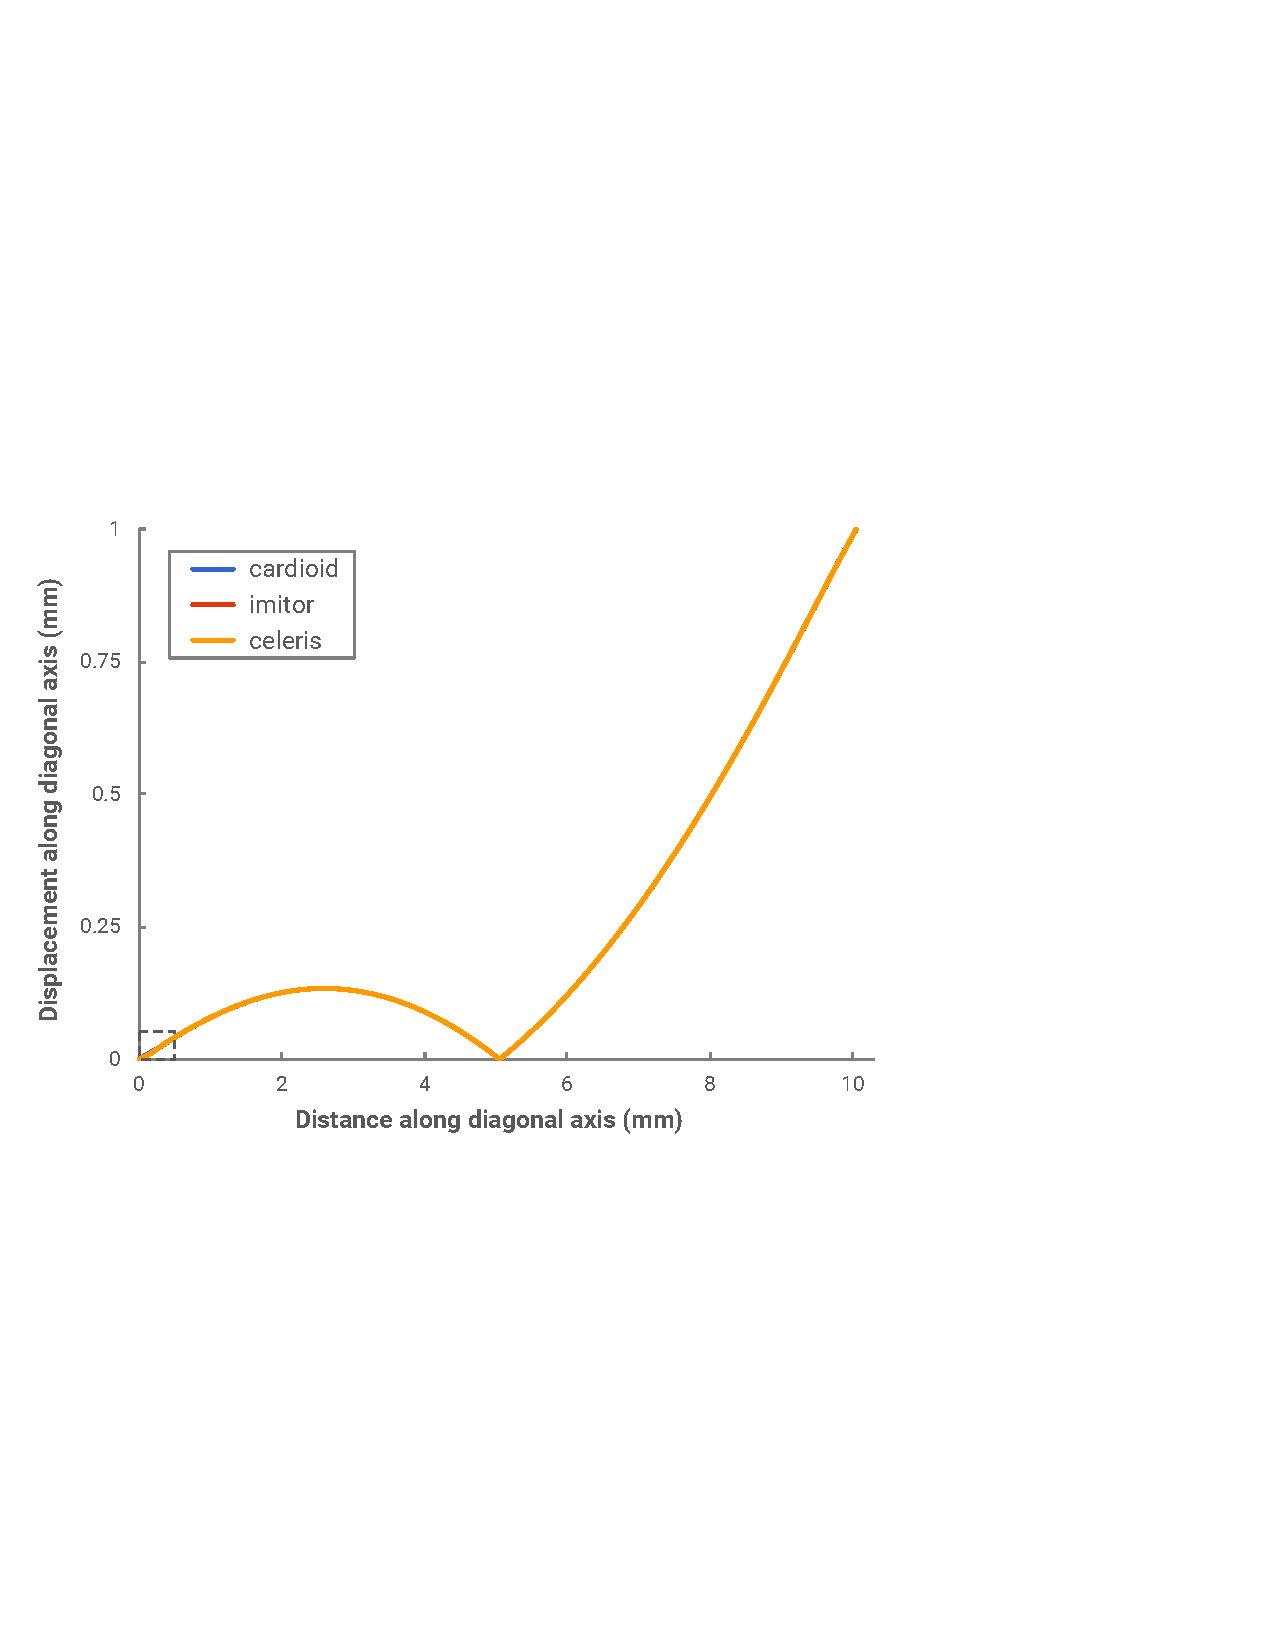
\includegraphics[scale=0.46]{media/5-verif/2-gurev3/gurev3-1.pdf}
\label{fig:gurev3-1}}		
\subfigure[]{%
		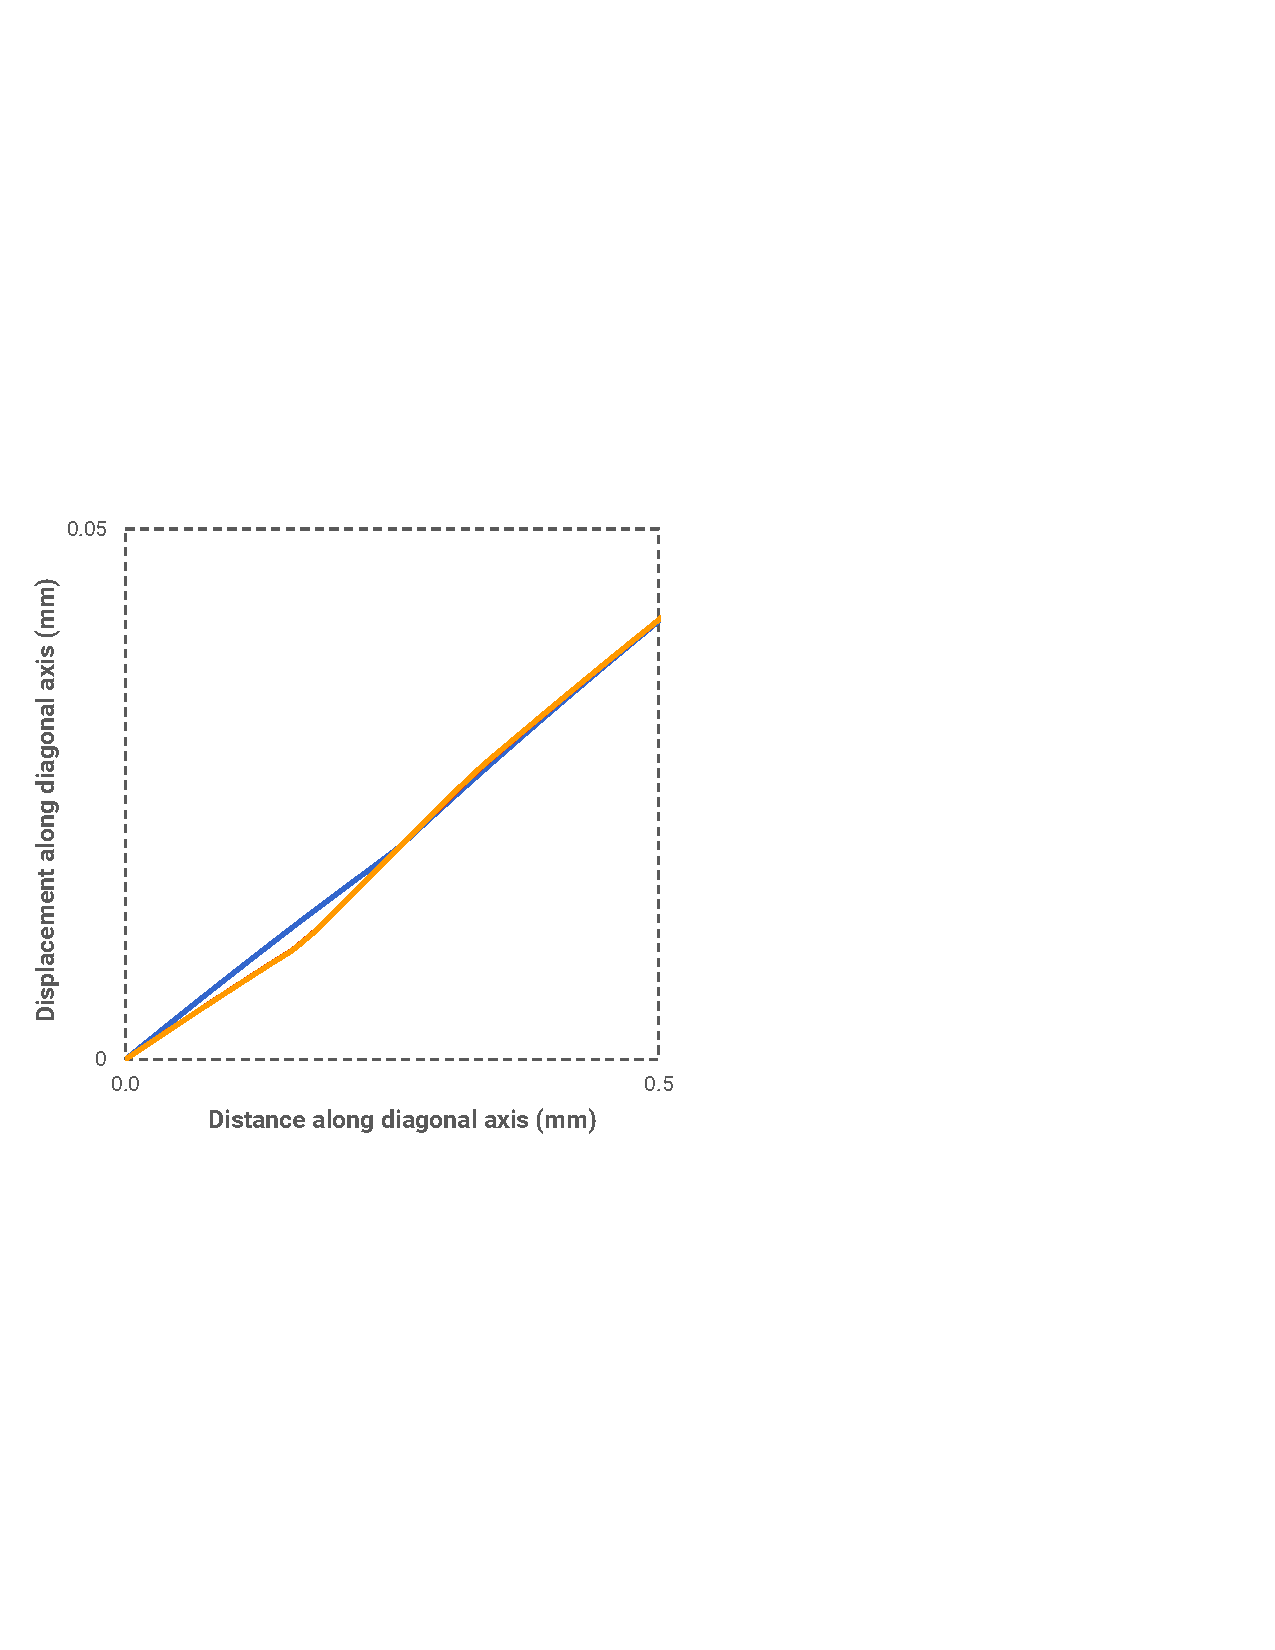
\includegraphics[scale=0.46]{media/5-verif/2-gurev3/gurev3-2.pdf}
\label{fig:gure3-2}}		
%
\caption{Results for Gurev P3 verification problem: (a) Displacement magnitude along diagonal axis, with (b) details for the fixed end of the beam. The results for imitor and Celeris are indistinguishable in these plots.}
\label{fig:gurev3}
\end{figure}

\begin{figure}[ht!]
\centering
\subfigure[]{%
		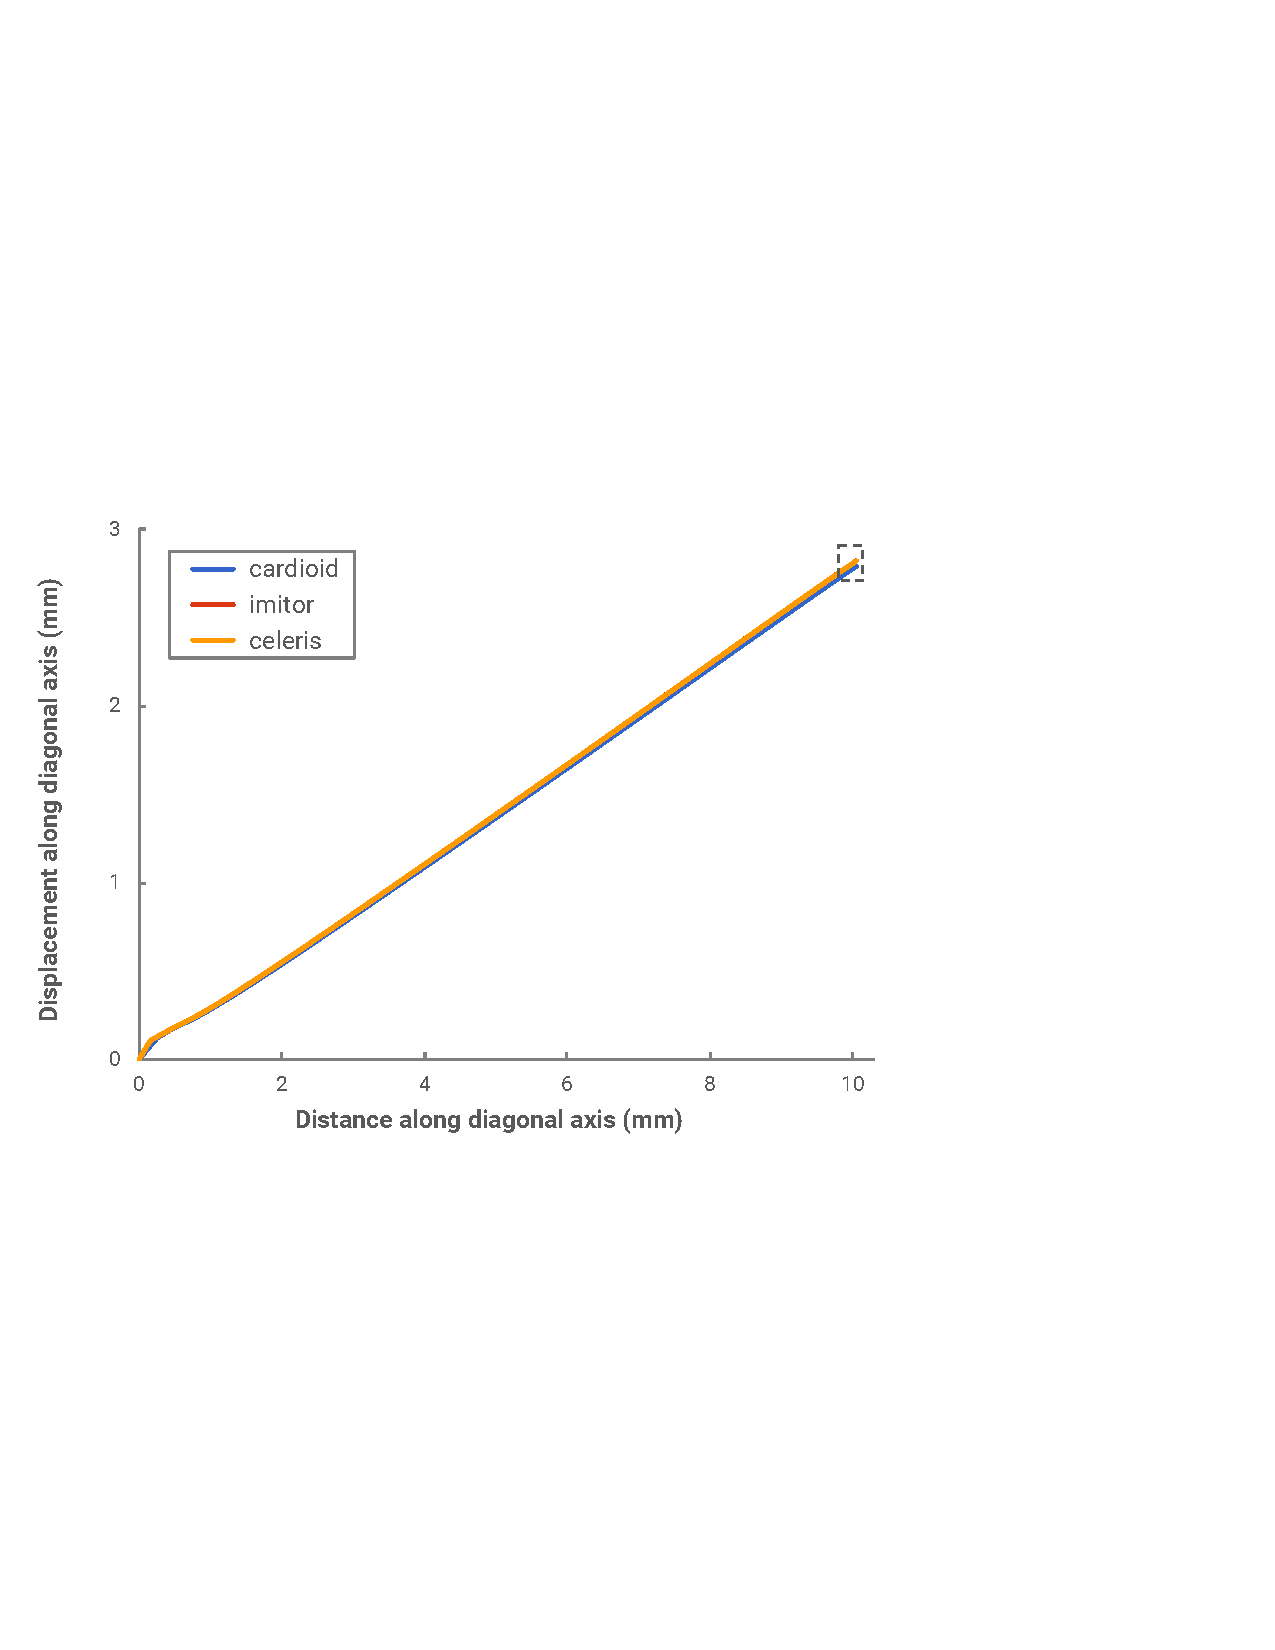
\includegraphics[scale=0.46]{media/5-verif/3-gurev4/gurev4-1.pdf}
\label{fig:gurev4-1}}		
\subfigure[]{%
		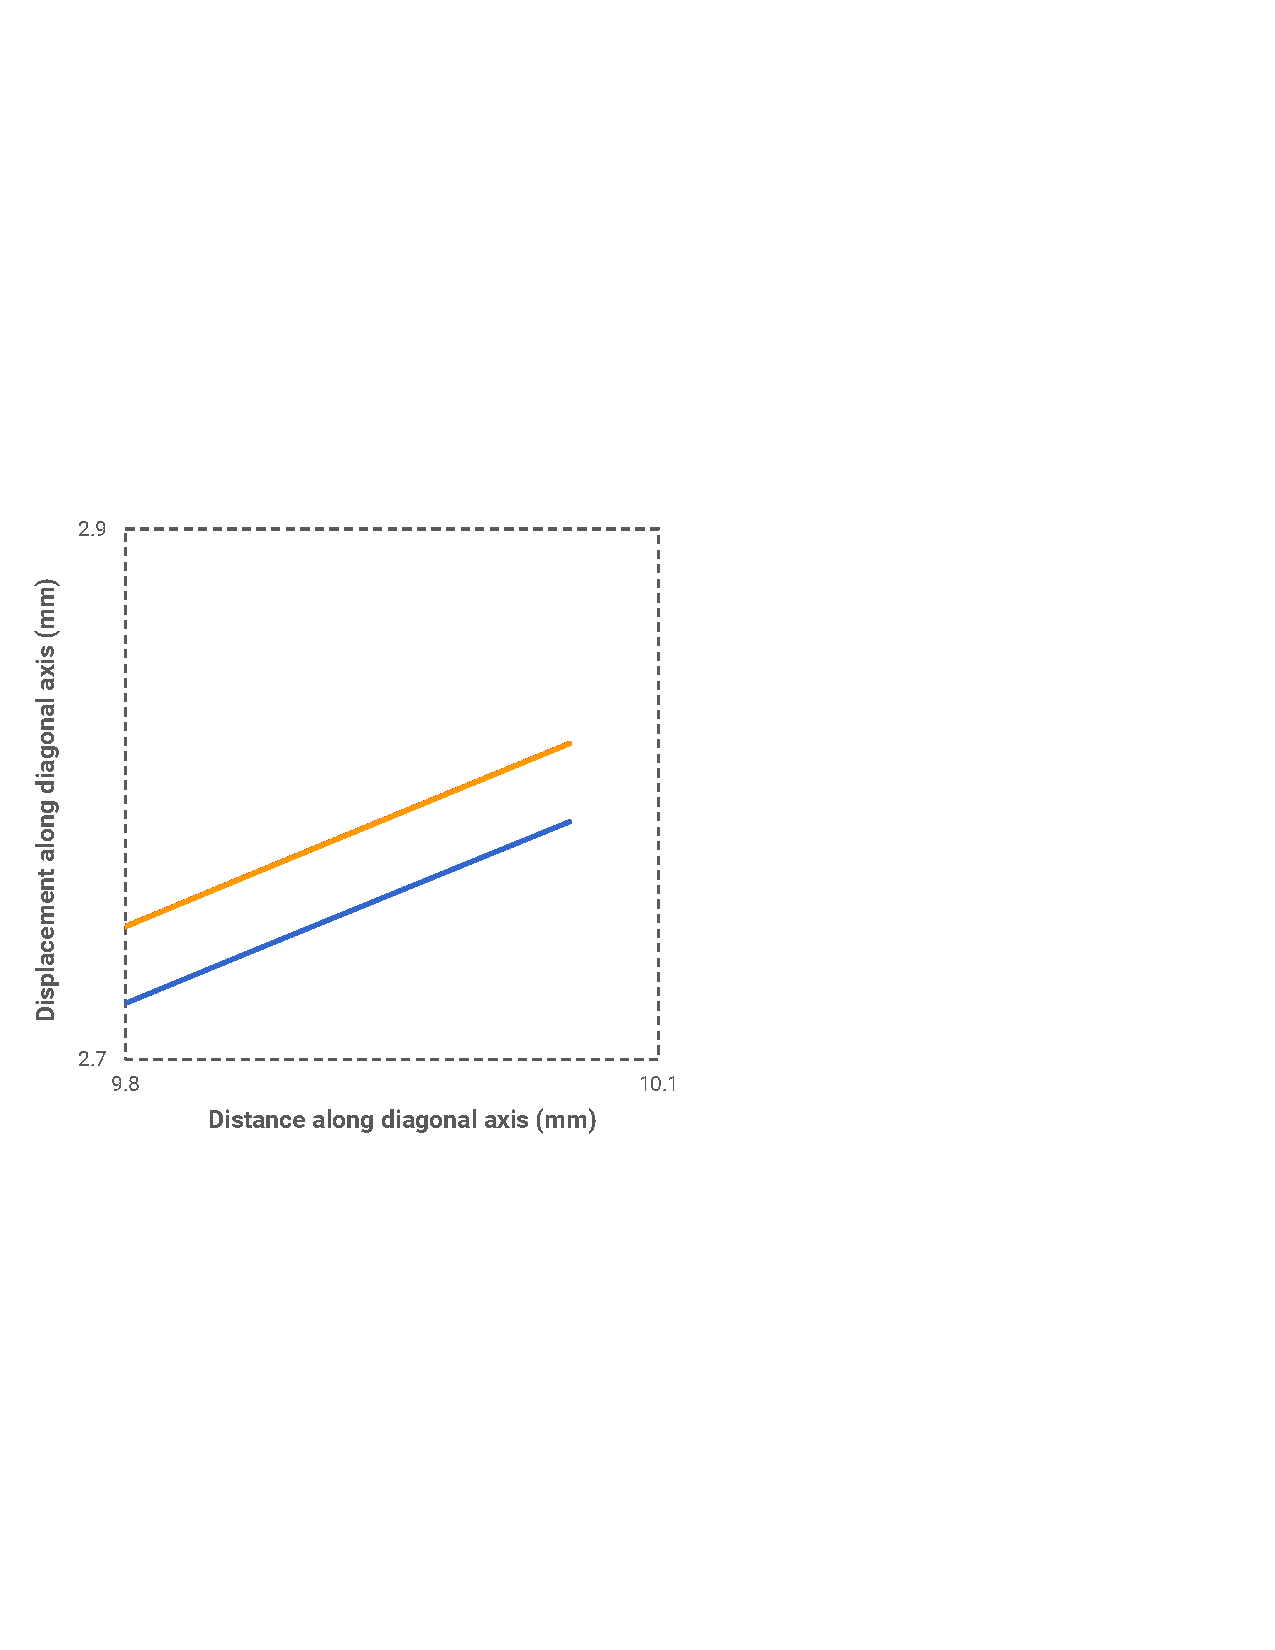
\includegraphics[scale=0.46]{media/5-verif/3-gurev4/gurev4-2.pdf}
\label{fig:gurev4-2}}		
%
\caption{Results for Gurev P4 verification problem: (a) Displacement magnitude along diagonal axis, with (b) details for the free end of the beam. The results for imitor and Celeris are indistinguishable in these plots.}
\label{fig:gurev4}
\end{figure}

\begin{figure}[ht!]
\centering
\subfigure[]{%
		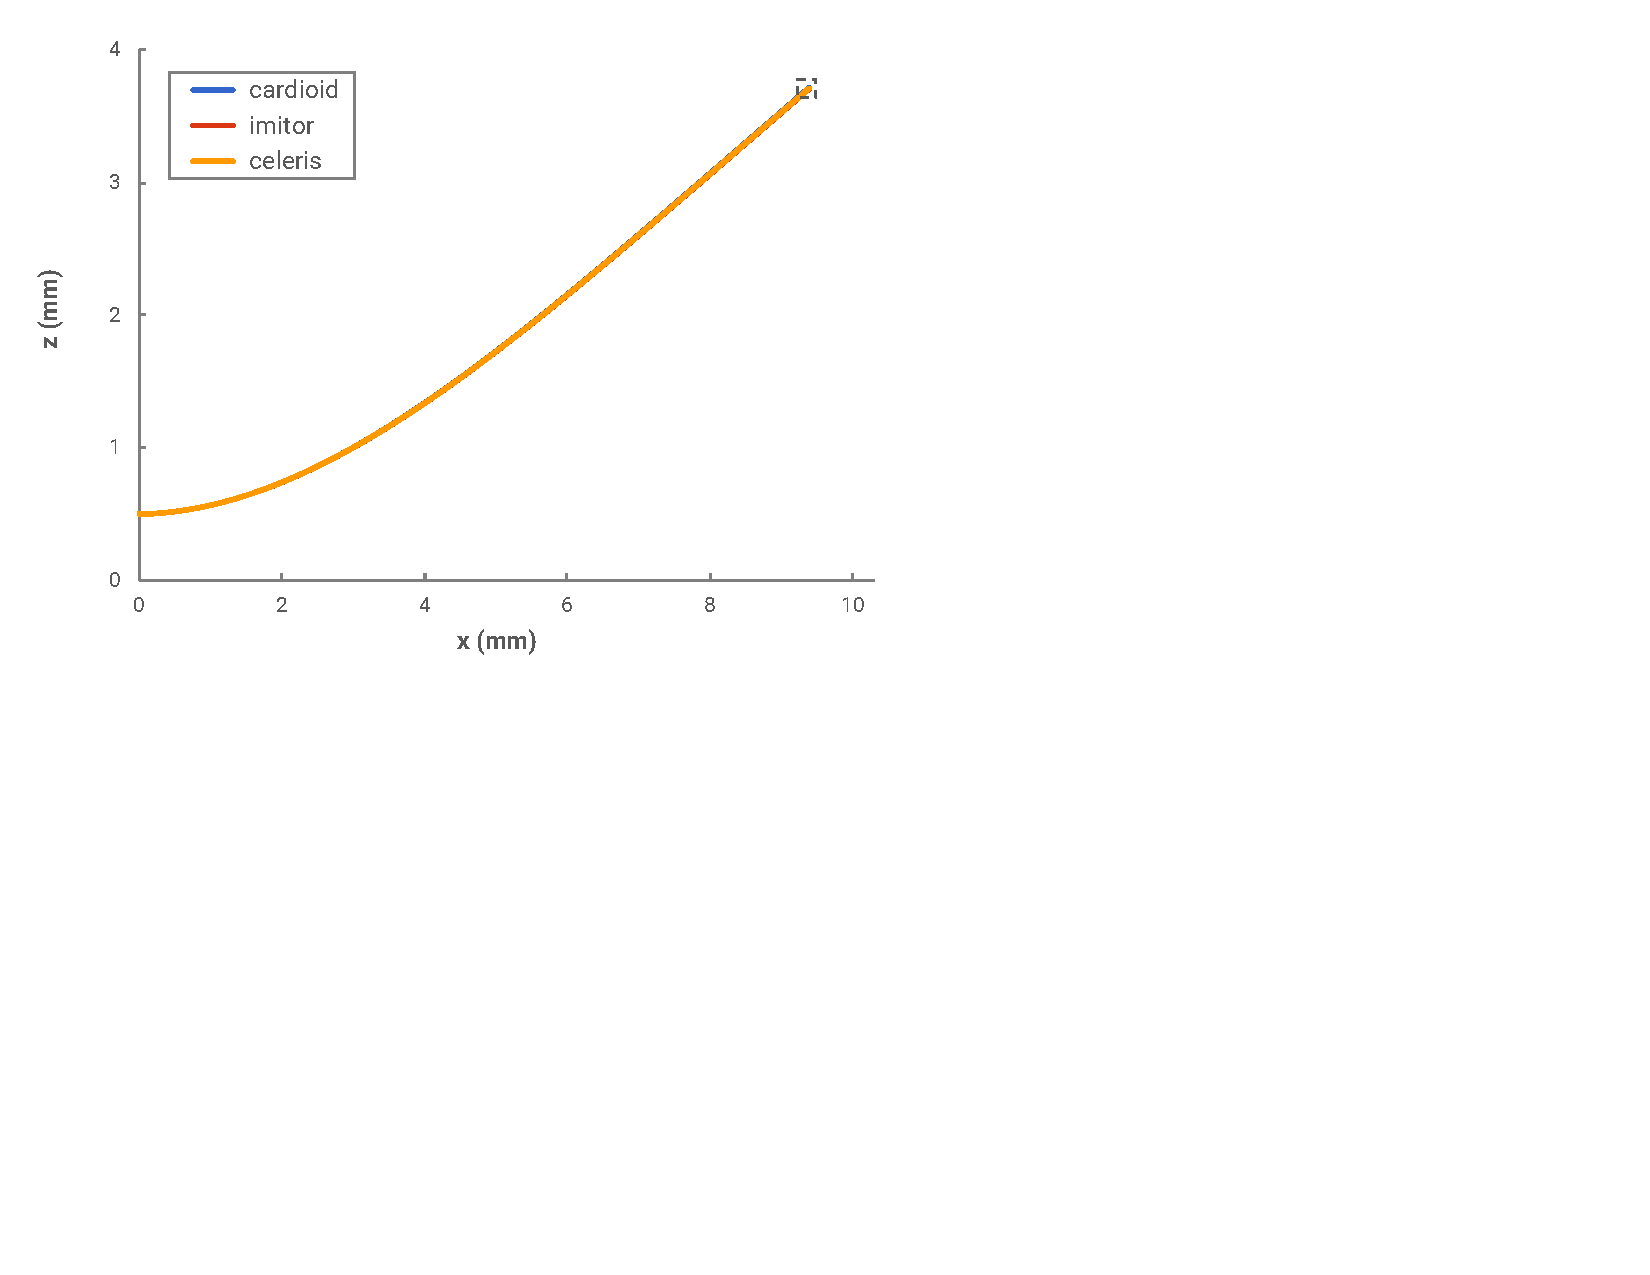
\includegraphics[scale=0.46]{media/5-verif/4-land1/land1-1.pdf}
\label{fig:land1-1}}		
\subfigure[]{%
		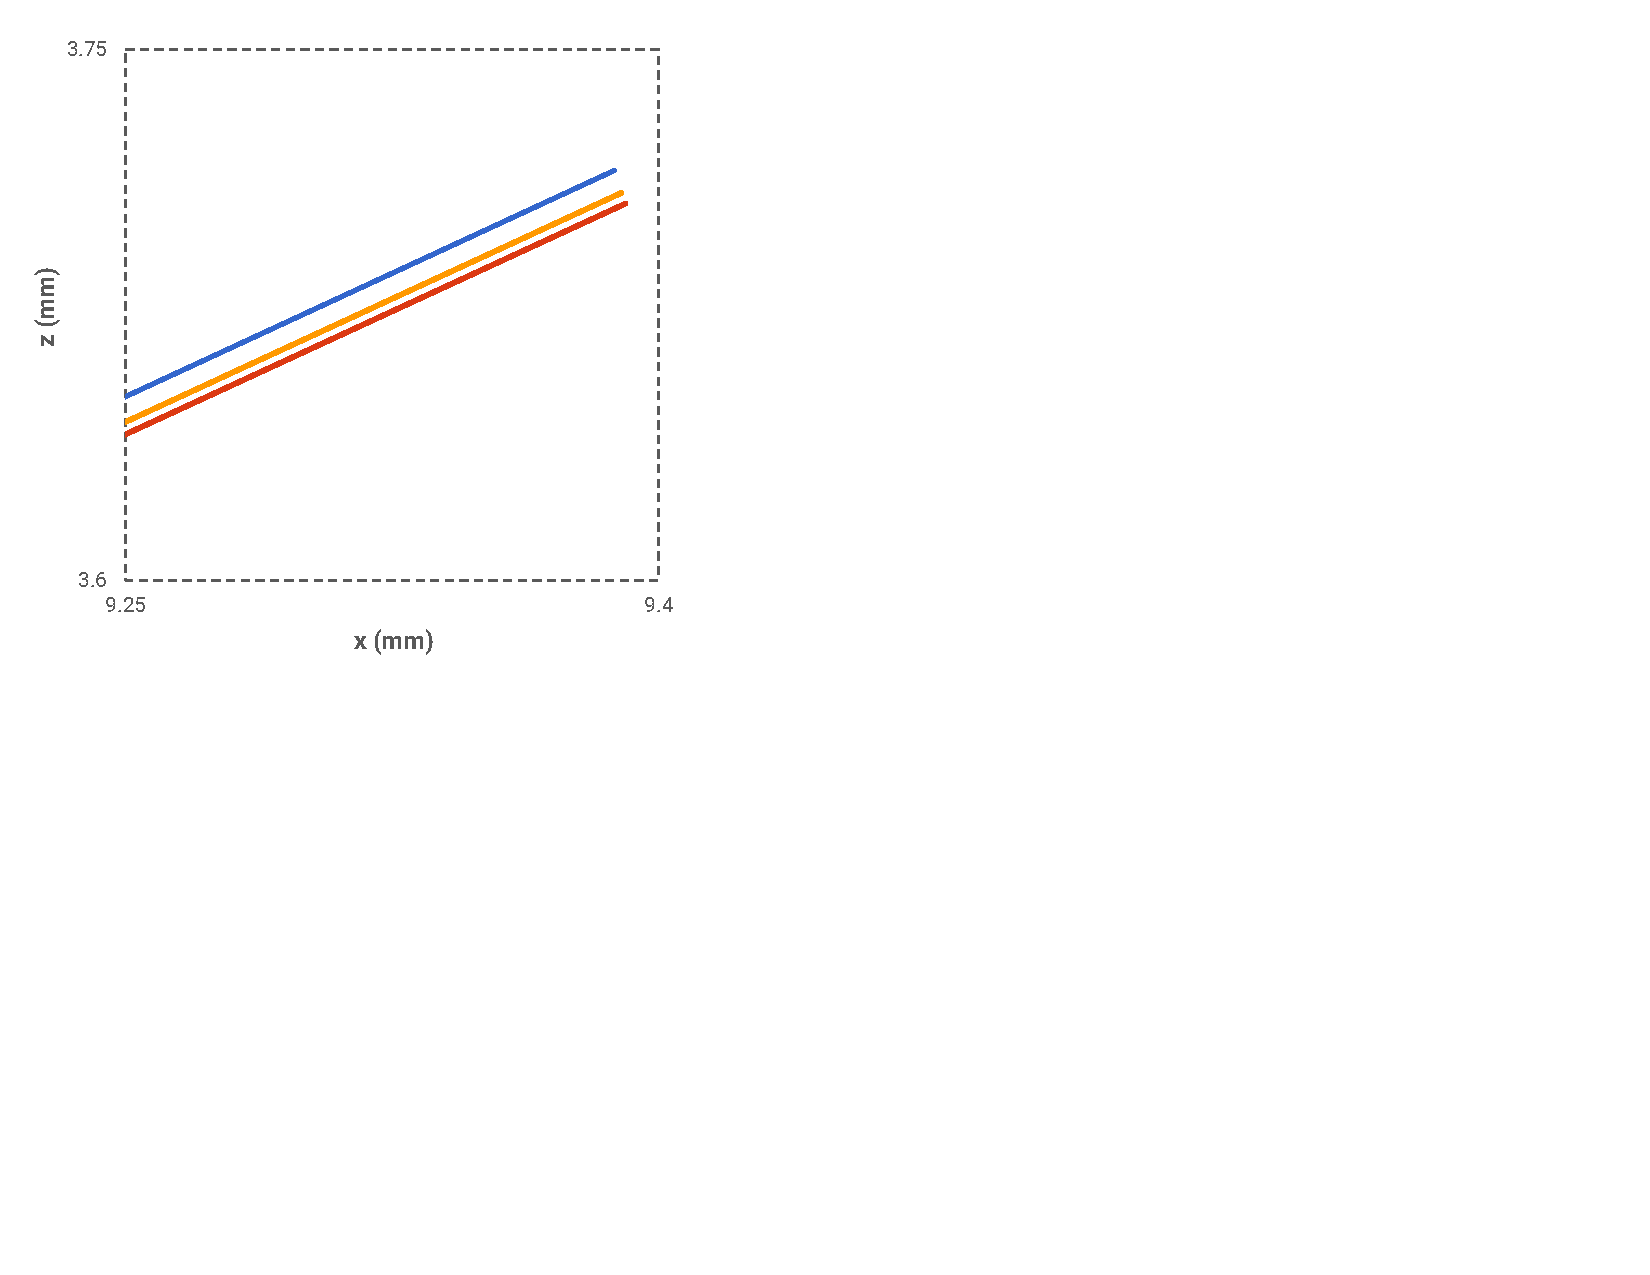
\includegraphics[scale=0.46]{media/5-verif/4-land1/land1-2.pdf}
\label{fig:land1-2}}	
\subfigure[]{%
		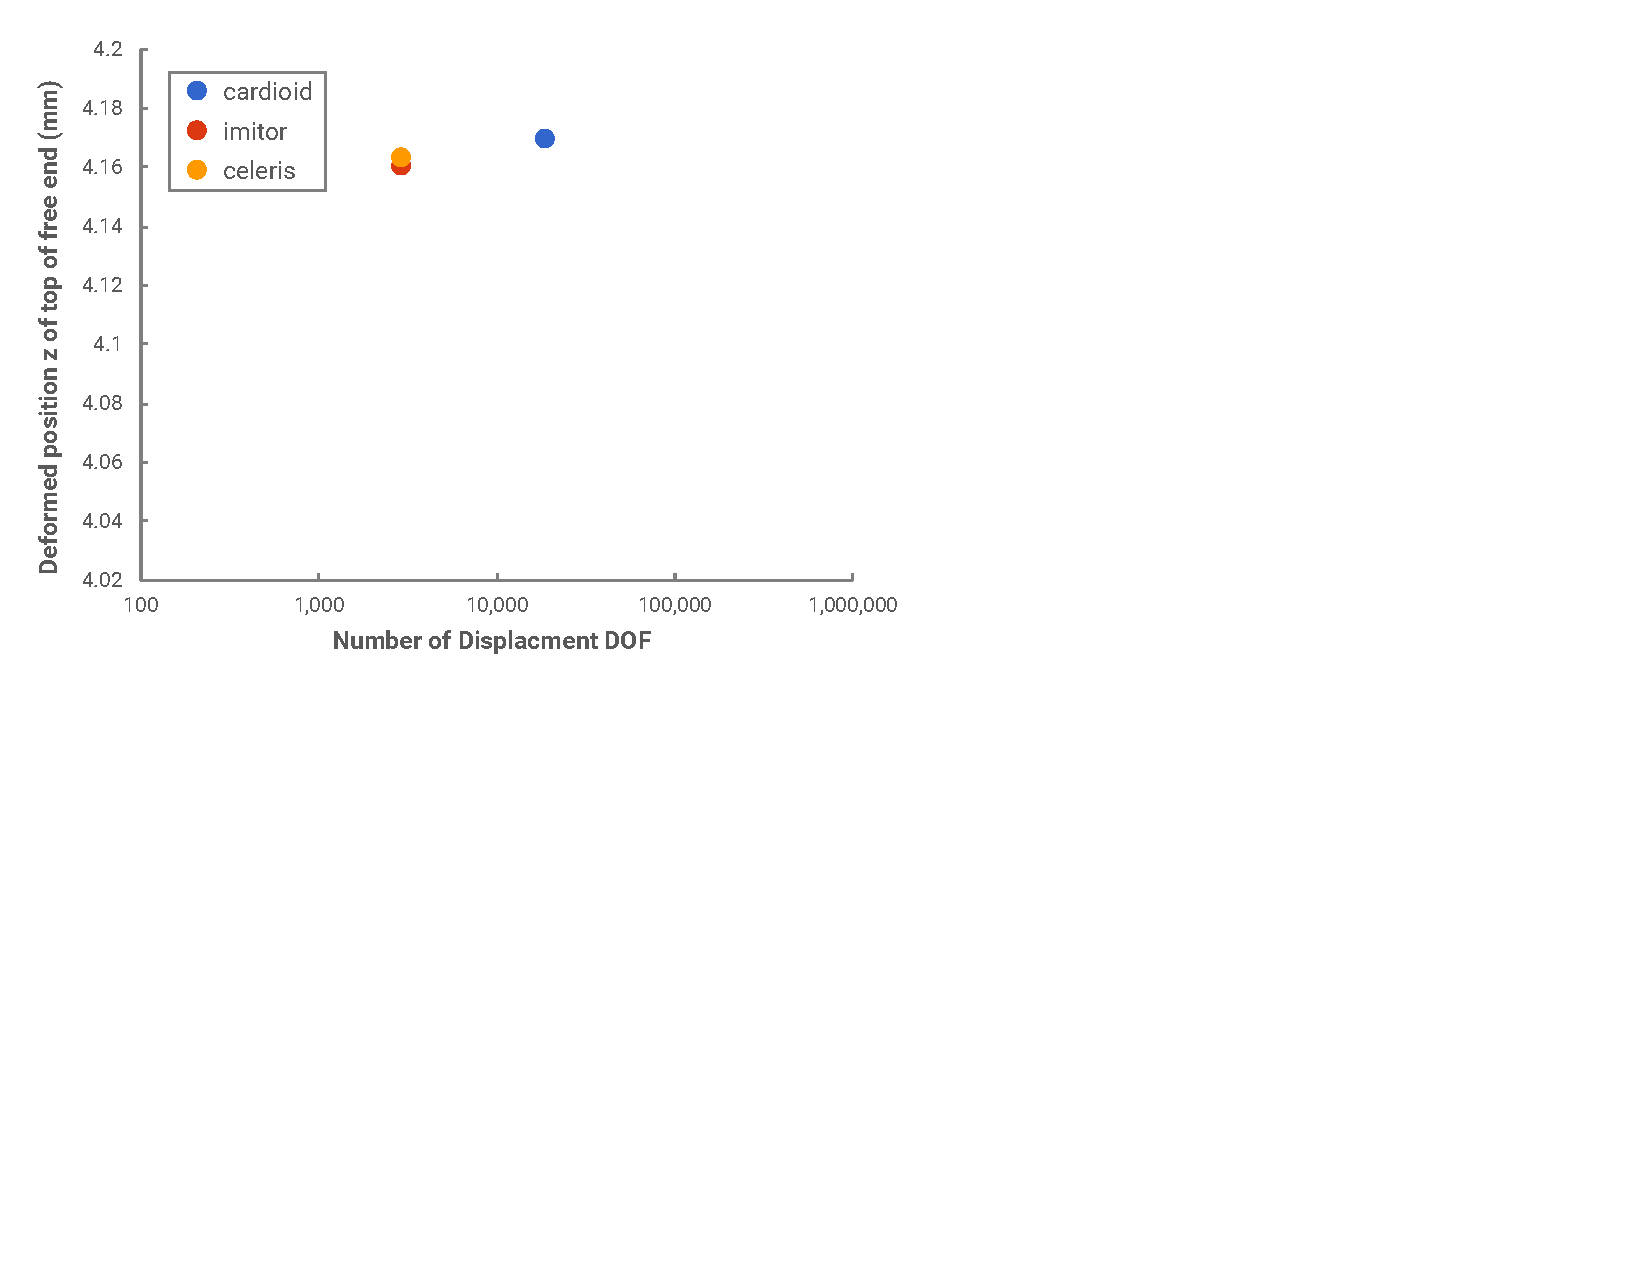
\includegraphics[scale=0.46]{media/5-verif/4-land1/land1-3.pdf}
\label{fig:land1-3}}			
%
\caption{Results for Land P1 verification problem: (a) Deformed position of midline, with (b) details for the free end of the beam. Panel (c) shows the deformed position of the point $\bm{X} = (10, 0.5, 1)$ for each of the simulation codes.}
\label{fig:land1}
\end{figure}


\begin{figure}[ht!]
\centering
\subfigure[]{%
		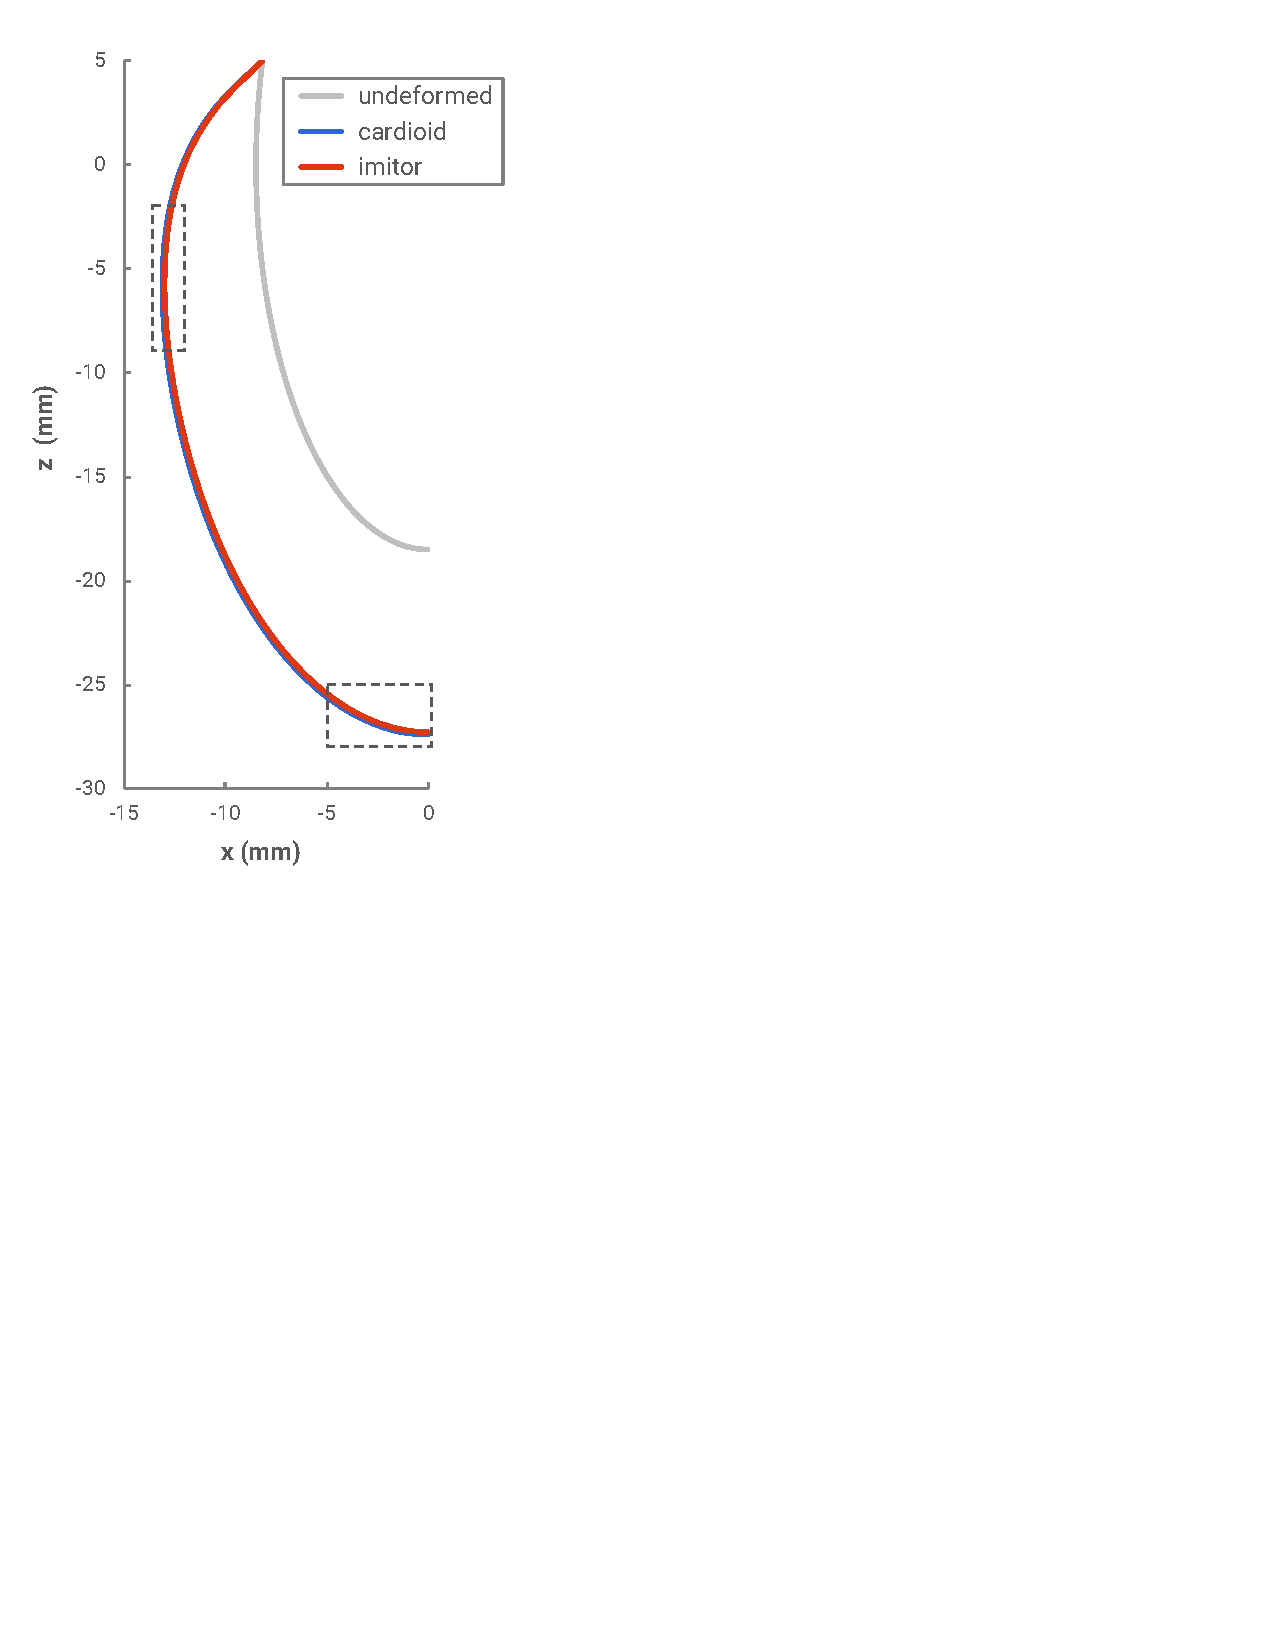
\includegraphics[scale=0.46]{media/5-verif/5-land2/land2-1.pdf}
\label{fig:land2-1}}		
\subfigure[]{%
		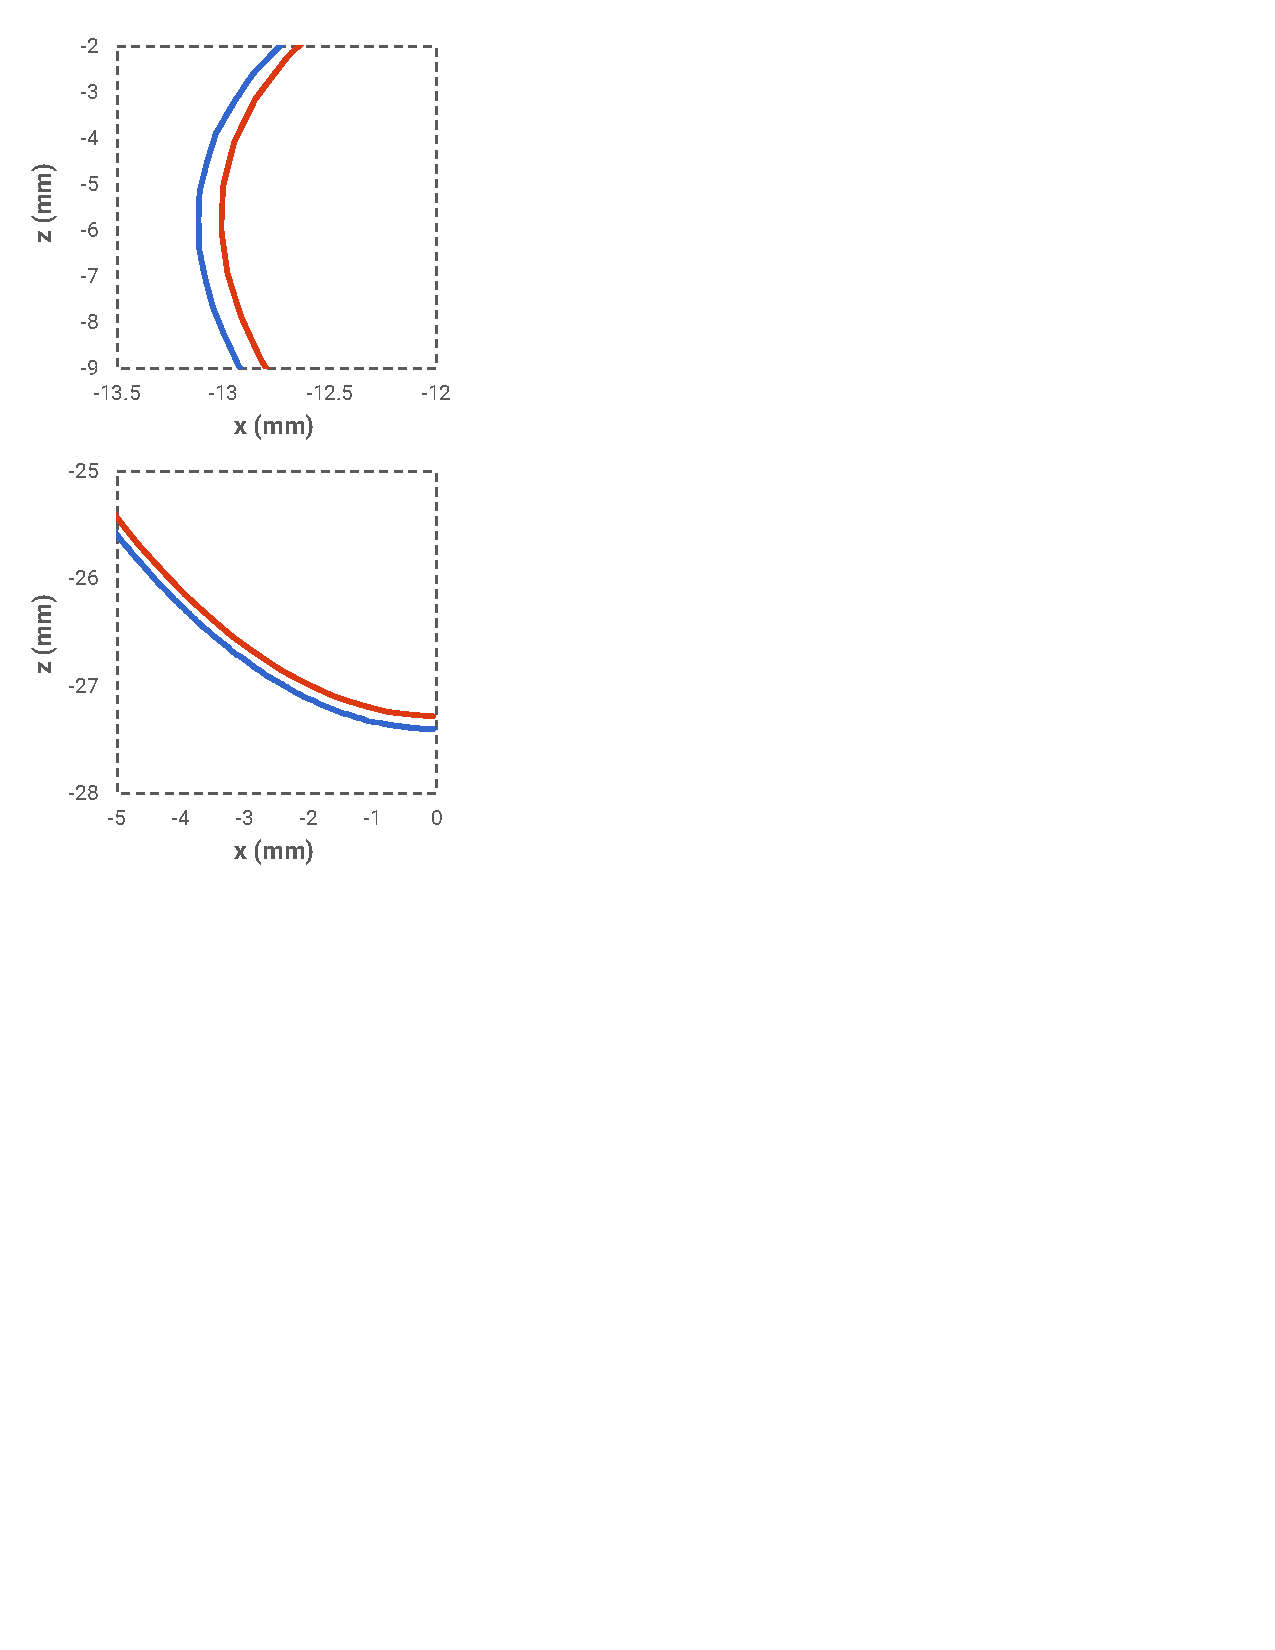
\includegraphics[scale=0.46]{media/5-verif/5-land2/land2-2.pdf}
\label{fig:land2-2}}	
\subfigure[]{%
		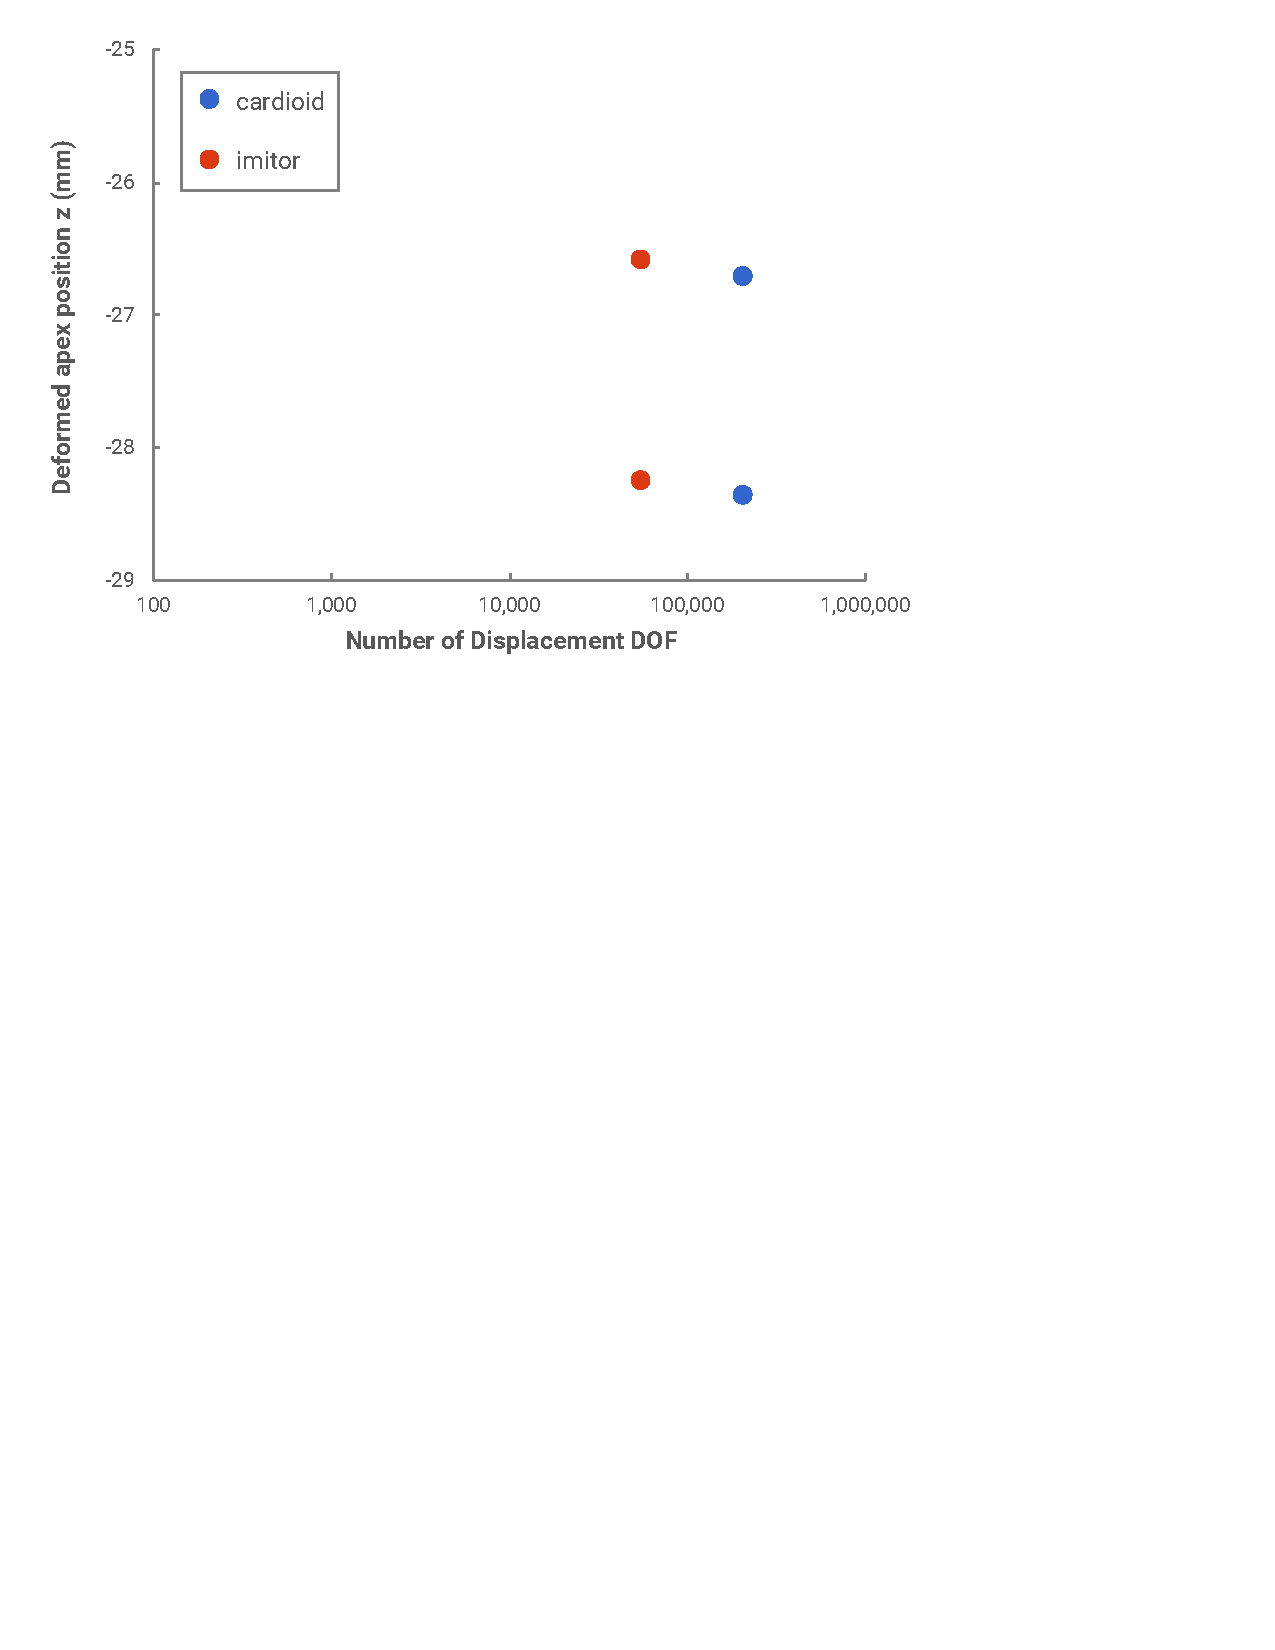
\includegraphics[scale=0.46]{media/5-verif/5-land2/land2-3.pdf}
\label{fig:land2-3}}			
%
\caption{Results for Land P2 verification problem: (a) Deformed position of middle of the ventricle wall, with (b) details at the inflection point (top right) and the apical region (bottom right). Panel (c) shows the deformed position of the apex at the endo- and epicardium for each of the simulation codes.}
\label{fig:land2}
\end{figure}

\begin{figure}[ht!]
\centering
\subfigure[]{%
		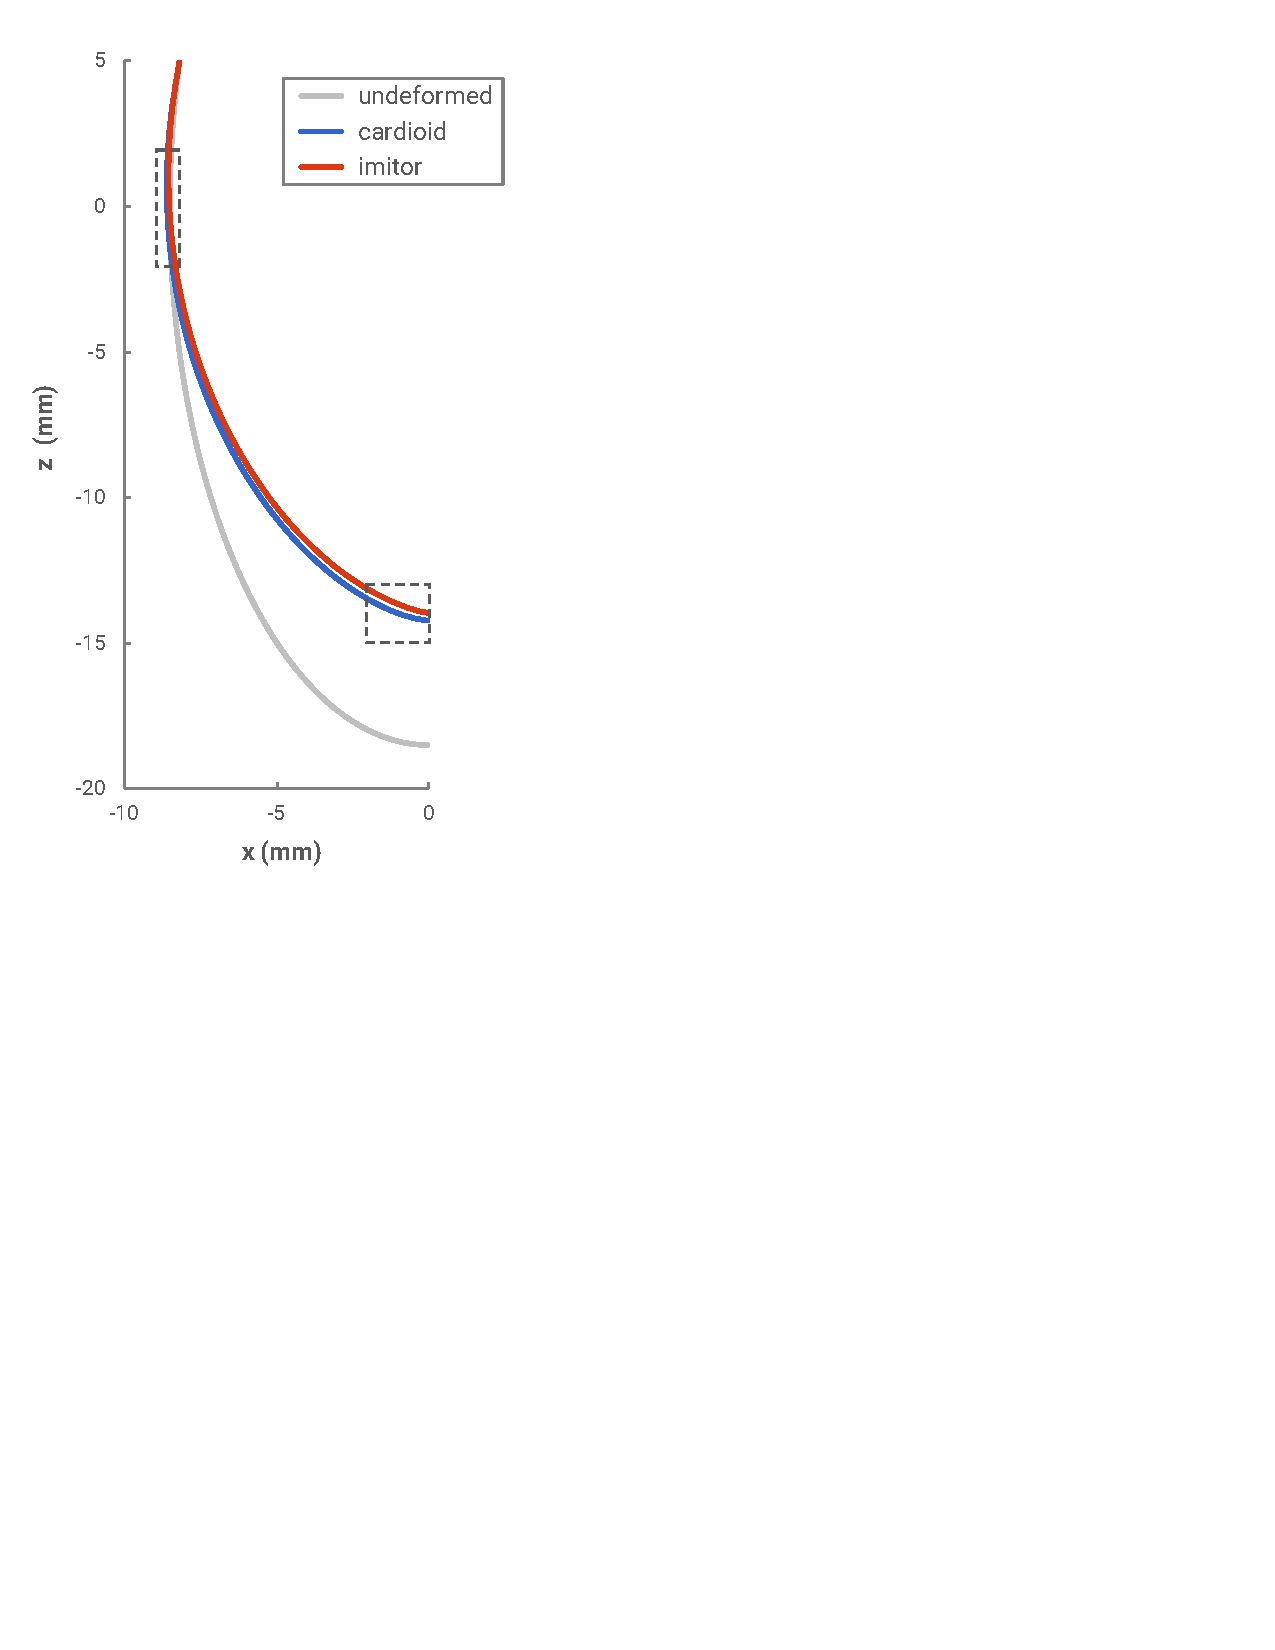
\includegraphics[scale=0.46]{media/5-verif/6-land3/land3-1.pdf}
\label{fig:land3-1}}		
\subfigure[]{%
		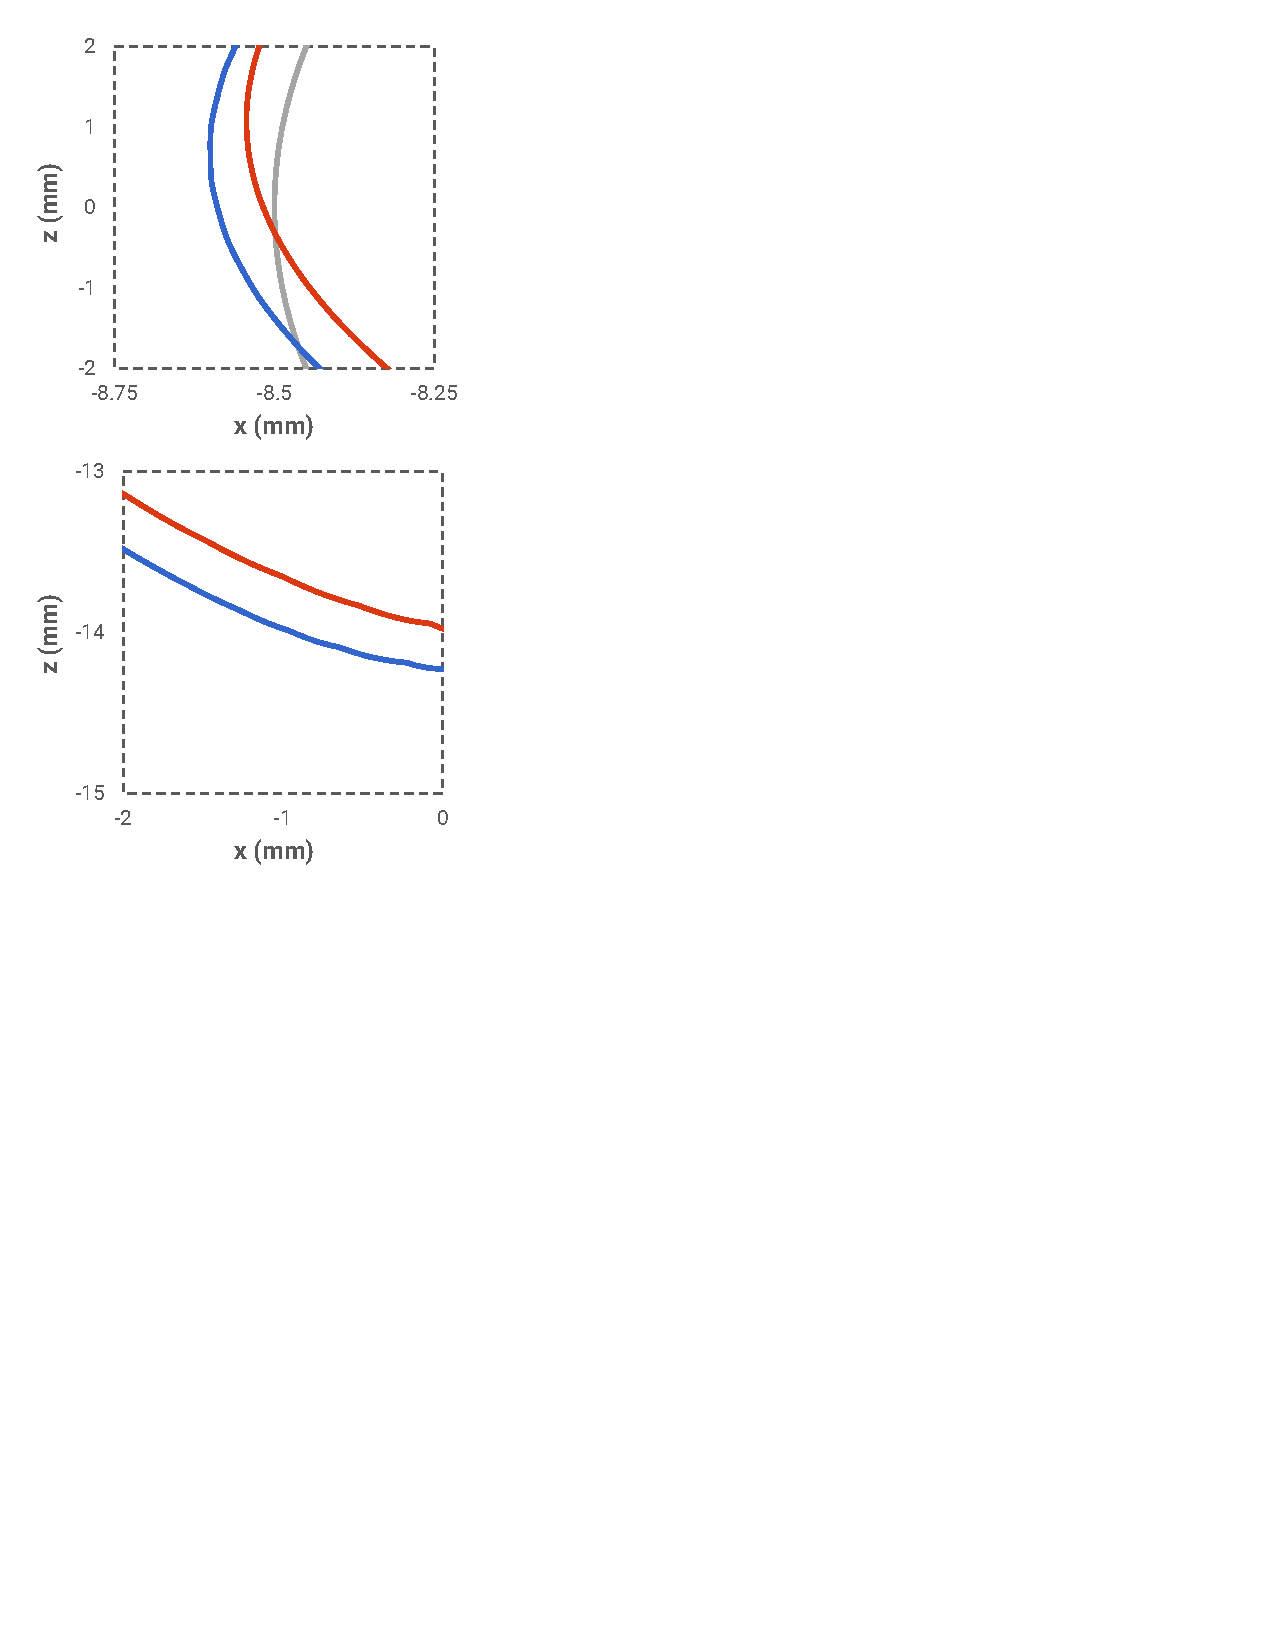
\includegraphics[scale=0.46]{media/5-verif/6-land3/land3-2.pdf}
\label{fig:land3-2}}	
%
\caption{Results for Land P3 verification problem: (a) Deformed position of middle of the ventricle wall, with (b) details at the inflection point (top right) and the apical region (bottom right).}
\label{fig:land3}
\end{figure}

\begin{figure}[ht!]
\centering
\subfigure[]{%
		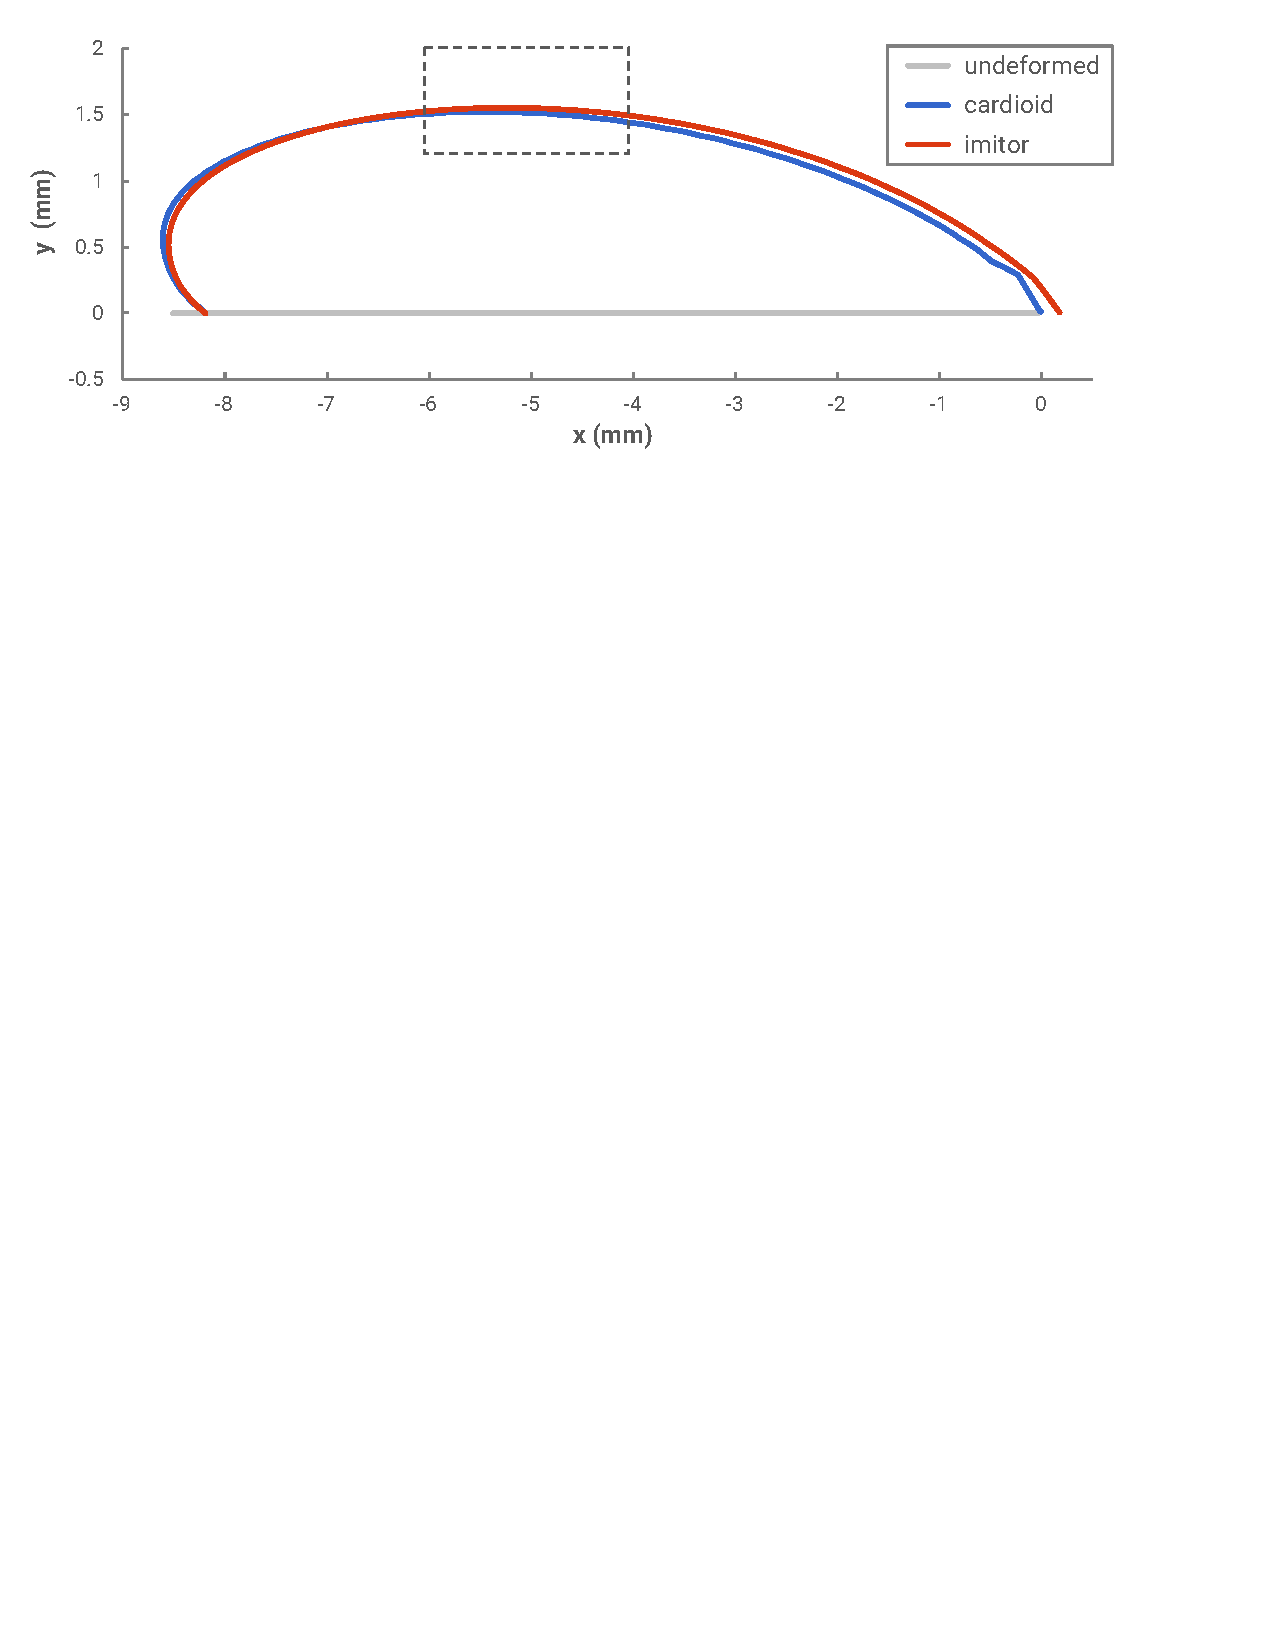
\includegraphics[scale=0.46]{media/5-verif/6-land3/land3-3.pdf}
\label{fig:land3.2-1}}		
\subfigure[]{%
		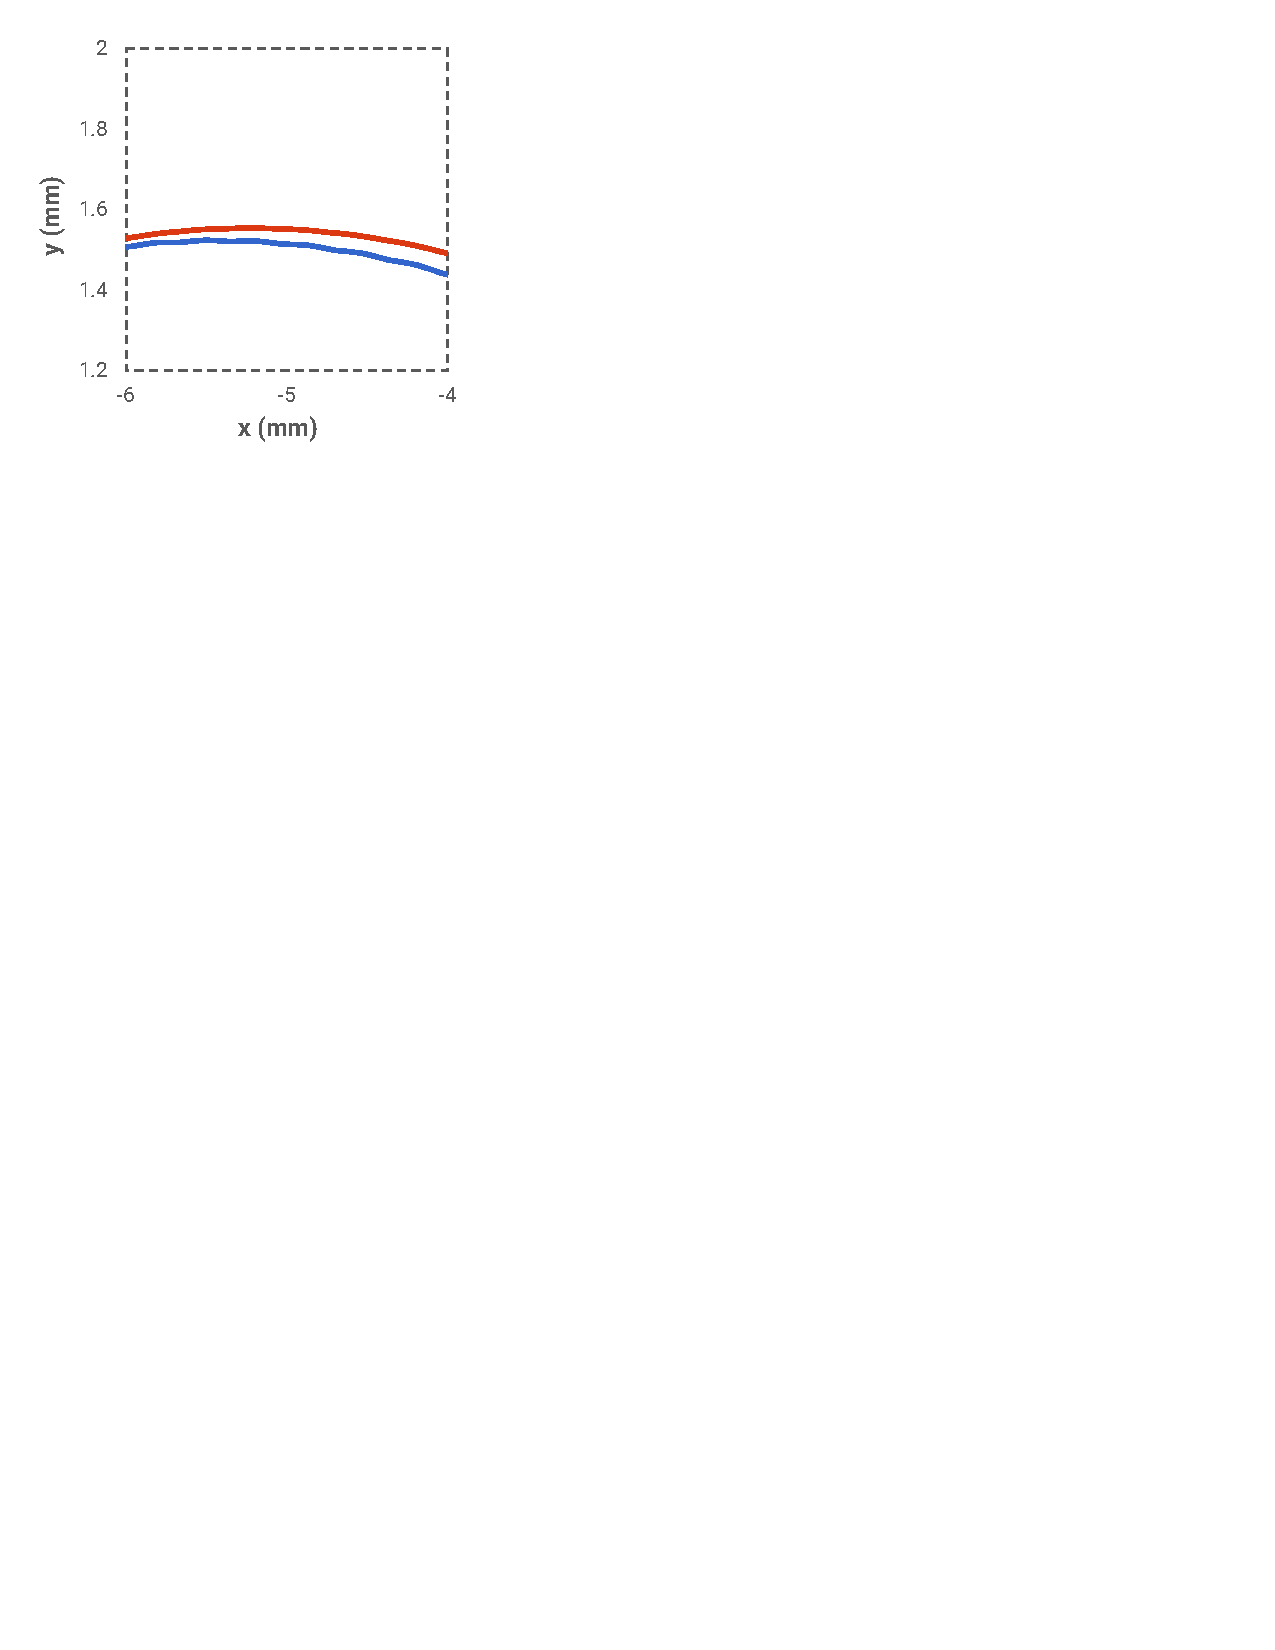
\includegraphics[scale=0.46]{media/5-verif/6-land3/land3-4.pdf}		
\label{fig:land3.2-2}}	
\subfigure[]{%
		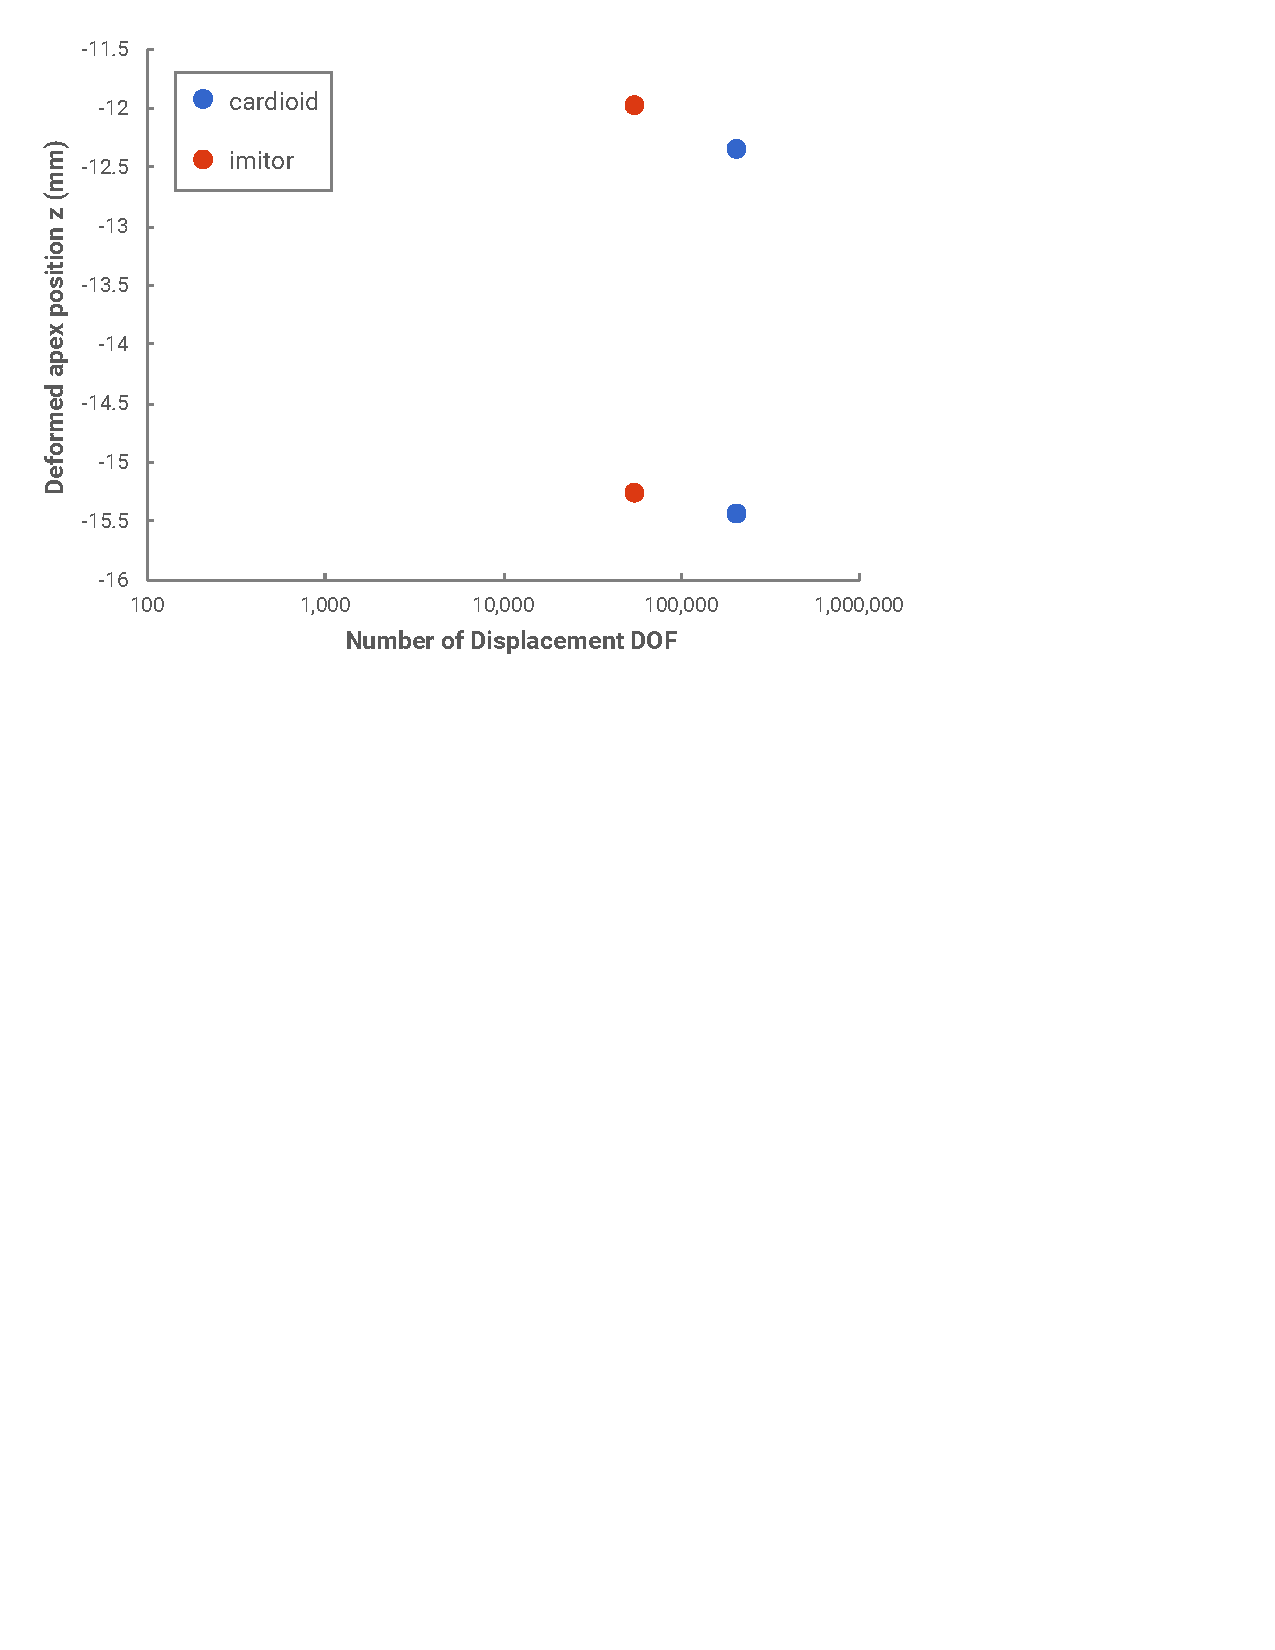
\includegraphics[scale=0.46]{media/5-verif/6-land3/land3-5.pdf}
\label{fig:land3.2-3}}			
	
%
\caption{Results for Land P3 verification problem: (a) The same deformed position of middle of the ventricle wall, shown in the $x-y$ plane, with (b) details at the inflection point. Panel (c) shows the deformed position of the apex at the endo- and epicardium for each of the simulation codes.}
\label{fig:land3.2}
\end{figure}
